%%%%%%%%%%%%%%%%%%%%%%%%%%%%%%%%%%%%%%%%%%%%%%%%%
%%%%%%%%%%%%%%%%%%%%%%%%%%%%%%%%%%%%%%%%%%%%%%%%%
%%% Maxime Ulysse Garcia, max@ithake.eu, 2013 %%%
%%%                                           %%%
%%%    Questions and suggestions WELCOMED!    %%%
%%%                                           %%%
%%% This thesis template largely derives from %%%
%%%      Charles Chapple, Robert Castelo      %%%
%%%    Sergio Mendoza and Sergi Castellano    %%%
%%%       Under GNU/GPL copyleft license      %%%
%%%                                           %%%
%%%   FEEL FREE TO USE IT AND IMPROVE IT!!!   %%%
%%%                                           %%%
%%%%%%%%%%%%%%%%%%%%%%%%%%%%%%%%%%%%%%%%%%%%%%%%%
%%%%%%%%%%%%%%%%%%%%%%%%%%%%%%%%%%%%%%%%%%%%%%%%%

%%% Preamble: LaTeX parameters and extensions %%%

%%%%%%%%%%%%%%%%%%%%%%%%%%%%%%%%%%%%%%%%%%%%%%%%%
%%%%%%%%%%%%%%%%%%%%%%%%%%%%%%%%%%%%%%%%%%%%%%%%%
%%% Maxime Ulysse Garcia, max@ithake.eu, 2013 %%%
%%%                                           %%%
%%%    Questions and suggestions WELCOMED!    %%%
%%%                                           %%%
%%% This thesis template largely derives from %%%
%%%      Charles Chapple, Robert Castelo      %%%
%%%    Sergio Mendoza and Sergi Castellano    %%%
%%%       Under GNU/GPL copyleft license      %%%
%%%                                           %%%
%%%   FEEL FREE TO USE IT AND IMPROVE IT!!!   %%%
%%%                                           %%%
%%%%%%%%%%%%%%%%%%%%%%%%%%%%%%%%%%%%%%%%%%%%%%%%%
%%% Preamble: LaTeX parameters and extensions %%%
%%%%%%%%%%%%%%%%%%%%%%%%%%%%%%%%%%%%%%%%%%%%%%%%%

%%%%%%%%%%%%%%%%%%%%%%%%%%%%%%%%%%%%%%%%%%%%%%%%%
%%%               Document type               %%%
%%%%%%%%%%%%%%%%%%%%%%%%%%%%%%%%%%%%%%%%%%%%%%%%%
% While working to see output errors
%\documentclass[draft,pdftex,oneside]{book}

% To produce final printable version
\documentclass[pdftex,oneside]{book}

%%%%%%%%%%%%%%%%%%%%%%%%%%%%%%%%%%%%%%%%%%%%%%%%%
%%%              Tweaking errors              %%%
%%%%%%%%%%%%%%%%%%%%%%%%%%%%%%%%%%%%%%%%%%%%%%%%%

% To remove "No room for a new \dimen" when using tikz
\RequirePackage{etex}
% For fancyhdr
\setlength{\headheight}{13pt}

%%%%%%%%%%%%%%%%%%%%%%%%%%%%%%%%%%%%%%%%%%%%%%%%%
%%%             Our own style file            %%%
%%%%%%%%%%%%%%%%%%%%%%%%%%%%%%%%%%%%%%%%%%%%%%%%%

% Style file for this template myThesis.sty
\RequirePackage{myThesis}
\RequirePackage{newicktree}

%%%%%%%%%%%%%%%%%%%%%%%%%%%%%%%%%%%%%%%%%%%%%%%%%
%%%                   Colors                  %%%
%%%%%%%%%%%%%%%%%%%%%%%%%%%%%%%%%%%%%%%%%%%%%%%%%

\RequirePackage{color}
%#############################################################%
%#############################################################%
%###    Maxime U. Garcia, max.u.garcia@gmail.com,  01/2013 ###%
%###                                                       ###%
%###          Questions and suggestions WELCOMED!          ###%
%###                                                       ###%
%###       This thesis template largely derives from       ###%
%###            Charles Chapple, Robert Castelo            ###%
%###         Sergio Mendoza and Sergi Castellano           ###%
%###             Under GNU/GPL copyleft license            ###%
%###                                                       ###%
%###         FEEL FREE TO USE IT AND IMPROVE IT!!!         ###%
%#############################################################%
%#############################################################%

% HTML colors definition

% black+grey+white
\definecolor{mydarkgrey}    {HTML}{444444}
\definecolor{mygrey}       	{HTML}{666666}
\definecolor{mylightgrey}  	{HTML}{AAAAAA}

%Links
\definecolor{brickred}     	{HTML}{990000}
\definecolor{steelblue}    	{HTML}{005A82}

% red
\definecolor{mydarkred}    	{HTML}{AA0000}
\definecolor{myred}        	{HTML}{BB0000}
\definecolor{mylightred}   	{HTML}{C68D8D}

% orange
\definecolor{mydarkorange} 	{HTML}{CF5300}
\definecolor{myorange}     	{HTML}{FF7F00}
\definecolor{mylightorange}	{HTML}{FF9B82}

% yellow
\definecolor{mydarkyellow} 	{HTML}{CFAF00}
\definecolor{myyellow}     	{HTML}{E6C200}
\definecolor{mylightyellow}	{HTML}{FFFF99}

% green
\definecolor{mydarkgreen}  	{HTML}{005C00}
\definecolor{mygreen}      	{HTML}{009900}
\definecolor{mylightgreen} 	{HTML}{D7F3D7}

% blue
\definecolor{mydarkblue}   	{HTML}{111A4C}
\definecolor{myblue}       	{HTML}{073C85}
\definecolor{mylightblue}  	{HTML}{CBDCE5}

% indigo
\definecolor{mydarkindigo} 	{HTML}{4B0082}
\definecolor{myindigo}     	{HTML}{4B0082}
\definecolor{mylightindigo}	{HTML}{E4BFFE}

% violet
\definecolor{mydarkviolet} 	{HTML}{5C0099}
\definecolor{myviolet}     	{HTML}{5C0099}
\definecolor{mylightviolet}	{HTML}{FFC6FE}


%%%%%%%%%%%%%%%%%%%%%%%%%%%%%%%%%%%%%%%%%%%%%%%%%
%%%                Paper layout               %%%
%%%%%%%%%%%%%%%%%%%%%%%%%%%%%%%%%%%%%%%%%%%%%%%%% 

\RequirePackage[paperwidth=170mm,paperheight=240mm,hmargin={2cm,1cm},vmargin={2cm,1.75cm},headheight=14pt]{geometry}

%%%%%%%%%%%%%%%%%%%%%%%%%%%%%%%%%%%%%%%%%%%%%%%%%
%%%                  Headings                 %%%
%%%%%%%%%%%%%%%%%%%%%%%%%%%%%%%%%%%%%%%%%%%%%%%%%

%For memoir class
\let\footruleskip\undefined

% To produce nice headings
\RequirePackage{fancyhdr}
\pagestyle{fancy} 

% Big first letter.
\RequirePackage{lettrine}
\newcommand{\mylettrine}[1]{\lettrine[lines=4,loversize=-0.1,lraise=0.1,lhang=.2]{#1}}

%%%%%%%%%%%%%%%%%%%%%%%%%%%%%%%%%%%%%%%%%%%%%%%%%
%%%            Marks and draftmarks           %%%
%%%%%%%%%%%%%%%%%%%%%%%%%%%%%%%%%%%%%%%%%%%%%%%%%

\newcommand{\myversion}{V 0.5}

\renewcommand{\chaptermark}[1]{\markboth{\thechapter. #1}{}}
\renewcommand{\sectionmark}[1]{\markright{\thesection\ #1}}

\lfoot{}
\rfoot{}

% Normal marks
%\lhead[\fancyplain{}{\sffamily\thepage}]{\fancyplain{}{\sffamily\rightmark}}
%\rhead[\fancyplain{}{\sffamily\leftmark}]{\fancyplain{}{\sffamily\thepage}}
%\cfoot{}

%Draftmarks
\lhead[\fancyplain{}{\sffamily\thepage}]{\fancyplain{}{\sffamily\textcolor{blue}{DRAFT} \rightmark}}
\rhead[\fancyplain{}{\sffamily\leftmark}]{\fancyplain{}{\sffamily\textcolor{blue}{\today} \thepage}}
\cfoot{\textcolor{blue}{\myversion}}

%%% Line Spacing %%%
\RequirePackage{setspace}

%%%%%%%%%%%%%%%%%%%%%%%%%%%%%%%%%%%%%%%%%%%%%%%%%
%%%                PDF commands               %%%
%%%%%%%%%%%%%%%%%%%%%%%%%%%%%%%%%%%%%%%%%%%%%%%%%

% To produce final version
\RequirePackage{pdfpages}

% Used in each \%includepdf call unless overwritten locally
\includepdfset{frame=false,pagecommand={\thispagestyle{fancy}}}

%%%%%%%%%%%%%%%%%%%%%%%%%%%%%%%%%%%%%%%%%%%%%%%%%
%%%                  Figures                  %%%
%%%%%%%%%%%%%%%%%%%%%%%%%%%%%%%%%%%%%%%%%%%%%%%%%

% Path to figures
\graphicspath{{figures//}}
% To include graphics
\RequirePackage{graphicx}
% To wrap text
\RequirePackage{wrapfig}
% to draw Figures
\RequirePackage{tikz}
% to rotate figures and tables
\RequirePackage{rotating}

%%%%%%%%%%%%%%%%%%%%%%%%%%%%%%%%%%%%%%%%%%%%%%%%%
%%%                 Equations                 %%%
%%%%%%%%%%%%%%%%%%%%%%%%%%%%%%%%%%%%%%%%%%%%%%%%%

\RequirePackage{mathtools}

% Redefine the square root:
\let\oldsqrt\sqrt
\def\sqrt{\mathpalette\DHLhksqrt}
\def\DHLhksqrt#1#2{
  \setbox0=\hbox{$#1\oldsqrt{#2\,}$}\dimen0=\ht0
  \advance\dimen0-0.2\ht0
  \setbox2=\hbox{\vrule height\ht0 depth -\dimen0}
  {\box0\lower0.4pt\box2}}

%%%%%%%%%%%%%%%%%%%%%%%%%%%%%%%%%%%%%%%%%%%%%%%%%
%%%                Big numbers                %%%
%%%%%%%%%%%%%%%%%%%%%%%%%%%%%%%%%%%%%%%%%%%%%%%%%

\RequirePackage{numprint}

%%%%%%%%%%%%%%%%%%%%%%%%%%%%%%%%%%%%%%%%%%%%%%%%%
%%%                   Lists                   %%%
%%%%%%%%%%%%%%%%%%%%%%%%%%%%%%%%%%%%%%%%%%%%%%%%%

% Provides a new environnement to do a list
\newenvironment{mylist}[1]{%
  \begin{list}{}{%
    \settowidth{\labelwidth}{#1:}
    \setlength{\labelsep}{0.5cm}
    \setlength{\leftmargin}{\labelwidth}
    \addtolength{\leftmargin}{\labelsep}
    \setlength{\rightmargin}{0pt}
    \setlength{\parsep}{0.5ex plus 0.2ex minus 0.1ex}
    \setlength{\itemsep}{0 ex plus 0.2ex}
    \renewcommand{\makelabel}[1]{\textbf{##1}\hfil}
    }
  }
{\end{list}}

%%%%%%%%%%%%%%%%%%%%%%%%%%%%%%%%%%%%%%%%%%%%%%%%%
%%%                  Acronyms                 %%%
%%%%%%%%%%%%%%%%%%%%%%%%%%%%%%%%%%%%%%%%%%%%%%%%%

\RequirePackage{suffix}
\RequirePackage[printonlyused]{acronym}

%%%%%%%%%%%%%%%%%%%%%%%%%%%%%%%%%%%%%%%%%%%%%%%%%
%%%                  Verbatim                 %%%
%%%%%%%%%%%%%%%%%%%%%%%%%%%%%%%%%%%%%%%%%%%%%%%%%

\RequirePackage{moreverb}

%%%%%%%%%%%%%%%%%%%%%%%%%%%%%%%%%%%%%%%%%%%%%%%%%
%%%                 References                %%%
%%%%%%%%%%%%%%%%%%%%%%%%%%%%%%%%%%%%%%%%%%%%%%%%%

% Natural Sciences Citations: author-year and numerical citations
\RequirePackage[round,sort&compress]{natbib}

%%%%%%%%%%%%%%%%%%%%%%%%%%%%%%%%%%%%%%%%%%%%%%%%%
%%%                   Index                   %%%
%%%%%%%%%%%%%%%%%%%%%%%%%%%%%%%%%%%%%%%%%%%%%%%%%

% To make a subject index
\RequirePackage{makeidx}
\makeindex

%%%%%%%%%%%%%%%%%%%%%%%%%%%%%%%%%%%%%%%%%%%%%%%%%
%%%                   Fonts                   %%%
%%%%%%%%%%%%%%%%%%%%%%%%%%%%%%%%%%%%%%%%%%%%%%%%%

\RequirePackage{palatino}
\RequirePackage{amsfonts}

%%% to add an empty page, output pending figures and resume in an odd-numbered one %%%

\newcommand{\clearemptypage}{\newpage\thispagestyle{empty}\mbox{}}

\newcommand{\clearemptydoublepage}{
    \clearemptypage
    \if@twoside
        \ifodd
            \clearemptypage
        \fi
    \fi}

%%%%%%%%%%%%%%%%%%%%%%%%%%%%%%%%%%%%%%%%%%%%%%%%%
%%%               URL inclusion               %%%
%%%%%%%%%%%%%%%%%%%%%%%%%%%%%%%%%%%%%%%%%%%%%%%%%

\RequirePackage[pdftex,colorlinks=true,linkcolor=black,menucolor=red,pdfhighlight=/P,citecolor=steelblue,urlcolor=brickred,linktocpage=false]{hyperref}
%Enter URLs like this: \url{http://ithake.eu/}

%%%%%%%%%%%%%%%%%%%%%%%%%%%%%%%%%%%%%%%%%%%%%%%%%
%%%               Defining terms              %%%
%%%%%%%%%%%%%%%%%%%%%%%%%%%%%%%%%%%%%%%%%%%%%%%%%

\def\myauthor{Maxime U. Garcia}

\def\mytitlefr{Découverte de biomarqueurs prédictifs en cancer du sein par Intégration Transcrip\-tome-Interactome}

\def\mytitleen{Biomarkers discovery in breast cancer by Interactome-Transcriptome Integration}

\def\myabstractfr{Lorem ipsum dolor sit amet, consectetur adipisicing elit, sed do eiusmod tempor incididunt ut labore et dolore magna aliqua. Ut enim ad minim veniam, quis nostrud exercitation ullamco laboris nisi ut aliquip ex ea commodo consequat. Duis aute irure dolor in reprehenderit in voluptate velit esse cillum dolore eu fugiat nulla pariatur. Excepteur sint occaecat cupidatat non proident, sunt in culpa qui officia deserunt mollit anim id est laborum. Lorem ipsum dolor sit amet, consectetur adipisicing elit, sed do eiusmod tempor incididunt ut labore et dolore magna aliqua. Ut enim ad minim veniam, quis nostrud exercitation ullamco laboris nisi ut aliquip ex ea commodo consequat. Duis aute irure dolor in reprehenderit in voluptate velit esse cillum dolore eu fugiat nulla pariatur. Excepteur sint occaecat cupidatat non proident, sunt in culpa qui officia deserunt mollit anim id est laborum. Lorem ipsum dolor sit amet, consectetur adipisicing elit, sed do eiusmod tempor incididunt ut labore et dolore magna aliqua.}

\def\myabstracten{Lorem ipsum dolor sit amet, consectetur adipisicing elit, sed do eiusmod tempor incididunt ut labore et dolore magna aliqua. Ut enim ad minim veniam, quis nostrud exercitation ullamco laboris nisi ut aliquip ex ea commodo consequat. Duis aute irure dolor in reprehenderit in voluptate velit esse cillum dolore eu fugiat nulla pariatur. Excepteur sint occaecat cupidatat non proident, sunt in culpa qui officia deserunt mollit anim id est laborum. Lorem ipsum dolor sit amet, consectetur adipisicing elit, sed do eiusmod tempor incididunt ut labore et dolore magna aliqua. Ut enim ad minim veniam, quis nostrud exercitation ullamco laboris nisi ut aliquip ex ea commodo consequat. Duis aute irure dolor in reprehenderit in voluptate velit esse cillum dolore eu fugiat nulla pariatur. Excepteur sint occaecat cupidatat non proident, sunt in culpa qui officia deserunt mollit anim id est laborum. Lorem ipsum dolor sit amet, consectetur adipisicing elit, sed do eiusmod tempor incididunt ut labore et dolore magna aliqua.}

\def\mykeywordsfr{Transcriptome; Interactome; Intégration de données; Réseaux de gène; classification; SVM; Signature; Biomarqueurs; Cancer; Cancer du Sein}

\def\mykeywordsen{Transcriptome; Interactome; Data Integration; Gene Networks; classification; SVM; Signature; Biomarkers; Cancer; Breast Cancer}

% To get subscript easily
\newcommand{\textunderscript}[1]{$_{\text{#1}}$}

% To get e and er in superscript easily
\newcommand{\eme}{\textsuperscript{e} }
\newcommand{\er}{\textsuperscript{er} }

% To get CO2 and O2 easily
\newcommand{\COO}{CO\textunderscript{2} }
\newcommand{\OO}{O\textunderscript{2} }

% shorther command for boldface
\newcommand{\bb}[1]{\textbf{#1}}

%%%%%%%%%%%%%%%%%%%%%%%%%%%%%%%%%%%%%%%%%%%%%%%%%
%%%                 PDF infos                 %%%
%%%%%%%%%%%%%%%%%%%%%%%%%%%%%%%%%%%%%%%%%%%%%%%%%

\hypersetup{
    pdftitle        = {\mytitlefr},
    pdfsubject      = {Thèse de doctorat en Bioinformatique et Génomique à Aix-Marseille Université},
    pdfkeywords     = {\mykeywordsfr},
    pdfauthor       = {\myauthor},
    pdfcreator      = {\LaTeX},
    pdfproducer     = {pdfeTeX-0.\the\pdftexversion\pdftexrevision}
    pdfpagemode     = FullScreen,
    pdffitwindow    = true}

\AtBeginDocument{\pdfpagewidth=176mm\pdfpageheight=250mm}

%%%%%%%%%%%%%%%%%%%%%%%%%%%%%%%%%%%%%%%%%%%%%%%%%
%%%                 Paragraphs                %%%
%%%%%%%%%%%%%%%%%%%%%%%%%%%%%%%%%%%%%%%%%%%%%%%%%

\setlength{\parskip}{1ex plus0.2ex minus0.2ex}

%%%%%%%%%%%%%%%%%%%%%%%%%%%%%%%%%%%%%%%%%%%%%%%%%
%%%                    Date                   %%%
%%%%%%%%%%%%%%%%%%%%%%%%%%%%%%%%%%%%%%%%%%%%%%%%%

\date{}
 
%%%%%%%%%%%%%%%%%%%%%%%%%%%%%%%%%%%%%%%%%%%%%%%%%
%%%                 Footnotes                 %%%
%%%%%%%%%%%%%%%%%%%%%%%%%%%%%%%%%%%%%%%%%%%%%%%%%

% Vertical spacing between footnotes
\setlength{\footnotesep}{2ex}

% Rule height, width and space
\renewcommand{\footnoterule}{\noindent\rule{5cm}{.1ex}\vspace{1.5ex}}

% That's all folks! % Call layout and other LaTeX parameters from file preamble.tex

%%% Body: actual text with some control commands %%%

%%%%%%%%%%%%%%%%%%%%%%%%%%%%%%%%%%%%%%%%%%%%%%%%%%
%%% The whole writing starts here divided into %%%
%%%   frontmatter, mainmatter and backmatter   %%%
%%%%%%%%%%%%%%%%%%%%%%%%%%%%%%%%%%%%%%%%%%%%%%%%%%

% Each \input command searches for a .tex file in a directory

% Build the minitoc
\dominitoc
\nomtcrule

% Set how many levels of subsections are listed in the Table Of Contents (TOC)
\setcounter{secnumdepth}{5}
\setcounter{tocdepth}{5}

% The main body lies within the \begin{document} and \end{document} commands.
\begin{document}

%%% frontmatter %%%
\frontmatter
\thispagestyle{empty}
  \begin{center}
    \avantgarLarge \acl{AMU}\\[1ex]
    \avantgar Faculté des Sciences de Luminy\\[1ex]
    \avantgar École Doctorale des Sciences de la Vie et de la Santé\\[3ex]
  \end{center}

  \begin{flushright}
    \avantgar N\textsuperscript{o} attribué par la bibliothèque\\[1ex]
    \avantgar |\textunderscore|\textunderscore|\textunderscore|\textunderscore|\textunderscore|\textunderscore|\textunderscore|\textunderscore|\textunderscore|\textunderscore|\textunderscore|\textunderscore|\\[1ex]
  \end{flushright}

  \begin{center}
    \avantgarboldHuge THÈSE\\[1.5ex]

    \avantgarlarge Présentée en première version\\[1ex]
   %\avantgarlarge Présentée et soutenue publiquement\\[1ex]
    \avantgarlarge le 13 avril 2013 par\\[1ex]
    \avantgarLarge \myauthor\\[1ex]
    \avantgar Né le 14 mai 1982 à Arles (13)\\[5ex]

    \avantgarboldHuge \mytitlefr\\[2ex]

    \avantgarlarge Pour l'obtention du grade de\\[1ex]
    \avantgarLarge Docteur d'\acl{AMU}\\[1ex]
    \avantgarlarge Spécialité : Bioinformatique\\[5ex]

    \avantgarlarge Jury :\\[1ex]
    \begin{tabular}{llll}
      {\Large M.} & {\Large\textsc{Jacques van Helden}}  & {\large \acs{AMU} - \acs{TAGC}}  & {\large(Président)}   \\
      {\Large M.} & {\Large\textsc{Philippe Dessen}}     & {\large Génétiques des Tumeurs}  & {\large(Rapporteur)}  \\
      {\Large M.} & {\Large\textsc{Benno Schwikowski}}   & {\large Institut Pasteur}        & {\large(Rapporteur)}  \\
      {\Large M.} & {\Large\textsc{Pascal Barbry}}       & {\large \acs{IPMC}}              & {\large(Examinateur)} \\
      {\Large M.} & {\Large\textsc{François Bertucci}}   & {\large \acs{IPC}}               & {\large(Directeur)}   \\
      {\Large M.} & {\Large\textsc{Ghislain Bidaut}}     & {\large \acs{AMU} - \acs{CRCM}}  & {\large(Codirecteur)} \\
    \end{tabular}
  \end{center}
\clearemptypage

% Institutional logos and others
\thispagestyle{empty}
% Laboratory and intitutions
\noindent\textsf{Les travaux réalisés pendant cette thèse ont été effectués au \ac{CRCM} dans la \ac{Cibi}.\\Le \ac{CRCM} est une unité mixte de recherche affiliée à \acl{AMU} (\acs{AMU}) en tant qu'UM105, l'\ac{IPC}, l'\ac{INSERM} en tant qu'U1068 et le \ac{CNRS} en tant qu'UMR7258.}
\vspace{.7cm}

% Logos
\begin{center}
    \def\svgwidth{12cm}\input{figures/logoscol.pdf_tex}
\end{center}

% Funding
\vspace{.7cm}
\noindent\textsf{Les recherches réalisées pour cette thèse ont été financées par l'\ac{INCa} et l'\ac{INSERM}. Notre Cluster Beowulf est financé par la \ac{FRM}. Maxime U. Garcia a été financé par une bourse de thèse \ac{INSERM}/Région \ac{PACA} pendant ces travaux.}      
\clearemptypage

% Dedicatory
\thispagestyle{empty}

\vspace*{5cm}
% Dedicatory
\begin{flushright}
	\sffamily
		À ma famille\\
		À mes parents\\
		À Célia
\end{flushright} 
% Acknowledgements
\chapter*{Remerciements}

%(GB/FB + collaborateurs + Équipe + Labo + Amis + Famille)\dots
% Supervisors
\noindent{}Je voudrais tout d'abord exprimer mes plus profonds remerciements à Ghislan Bidaut sans qui cette thèse n'aurait pas eu lieu, et qui en plus d'un encadrement sans faille depuis le début a été une source de conseils tout au long de cette thèse. Je remercie de même François Bertucci pour toute l'aide qu'il a pu m'apporter, pour la rapidité et la justesse de ses réponses, ainsi que pour ses corrections à toutes heures. Je voudrais également remercier pour les conseils qu'elles m'ont apportées, toutes les personnes avec qui j'ai collaboré pour cette thèse : Daniel Birnbaum, Pascal Finetti, Arnaud Guille, Sabrina Carpentier, Raphaële Millat-Carus, Renaud Sabatier.
\vspace{.5cm}

% Team + Laboratory
\noindent{}Je tiens également à exprimer mes plus sincères remerciements à tous les membres présents et passés de la plateforme de Bioinformatique Intégrative du CRCM qui m'ont supporté malgré eux tout le long de ma thèse et de mon écriture : Samuel, Olivier, Alexandre, Fanny, Claire, Quentin, Julie, Guillaume. Je voudrais également inclure dans ces remerciements l'ensemble du CRCM : Françoise Birg et Jean-Paul Borg qui ont soutenu ce projet dès le début, Caroline pour avoir été un soutien moral sans faille, Sebastien, Will, Sebastien, Marie-José, Avais, MLA, MLT, Vincent, Javier, Émilie, Marion, Julien, Armelle, Axelle, Pascale, Bernard, Myriam, Julie, François, Laurence D, Laurence L et je présente mes excuses à tous ceux que j'aurais très probablement oublié\dots
\vspace{.5cm}

% New laboratory
\noindent{}Je voudrais également inclure dans ces remerciements mes nouveaux collègues du \acs{CSI} : Touati, Feroz, Baskar, Sarah et Marie-Pierre\dots
\vspace{.5cm}

% Friends
\noindent{}Je souhaite aussi adresser mes remerciements à tous mes amis : Éric, Alex, Greg, Olga, Benoit, Sabine, Duncan, Cyrille, Adrien, Yannick, Caro, Julie, Martin, Éric, Caroline, Antoine, Pierre, Ségolène, Benoit, Fabian, Stéphanie, Pierre-Henri, Gaëlle, Sebastien, Charlène, Muriel, Marion\dots
\vspace{.5cm}

% Family
\noindent{}J'exprime toute ma gratitude à mes parents Claude et Marie-Claude, mon frère Florent, Karine et leur trois enfants Robin, Thibaud et Tristan, ma grand-mère Jeane, mes oncles, tantes et cousins, ainsi qu'à toute la famille Ponniah\dots
\vspace{.5cm}

% Girlfriend...
\noindent{}Je conclurai en remerciant de tout mon c{\oe}ur Célia pour son aide et son soutien.

%%% TOC and List of figures and tables %%%

% For a more compact index layout 
\setlength{\parskip}{0.4ex plus0.2ex minus0.2ex}

% Main TOC
\tableofcontents
\mtcaddchapter %prevent shifting due to TOC, TOT and TOF

% Table of tables
\listoftables
\mtcaddchapter

% Table of figures
\listoffigures
\mtcaddchapter

%%% mainmatter %%%
\mainmatter
\clearemptydoublepage

% State of the art
\singlespacing

\mychapter{myred}{Introduction générale}
  \sectionred*{Résumé}
    \begin{center}
      \begin{tabular}{c}
        \fcolorbox{mydarkred}{mylightred}{
        \begin{minipage}[][4cm][c]{0.8\linewidth}
          \sffamily
          Ce chapitre introductif présente de façon génarale le cancer\index{cancer}.
          Après un court historique des différentes actions entamées contre cette maladie, nous explorerons les caractéristiques biologiques des cancers.
          Puis, nous détaillerons les spécificités du cancer du sein\index{cancer!cancer du sein}, avant d'aborder l'intérêt de la médecine prédictive et personnalisée pour les signatures prédictives de l'évolution des cancers, et ce plus spécifiquement dans le cadre du cancer du sein.
        \end{minipage}}\\
        \\[2ex]
        \begin{minipage}[][4cm][c]{0.9\linewidth}
          \mtcsetdepth{minitoc}{1}
          \minitoc
        \end{minipage}
      \end{tabular}
    \end{center}
    \newpage

  \doublespacing

  \section*{\textcolor{myred}{Problématique}}
    \mylettrine{L}{e cancer} est, dans les pays occidentalisés, la seconde cause de décès après les maladies cardio-vasculaires.
    Ceci en fait une préoccupation majeure de santé publique.
    En 1918, avec la création de La Ligue franco-anglo-américaine contre le cancer\footnote{actuellement La Ligue nationale contre le cancer}, une action associative est mise en place pour lutter contre le cancer.
    Les gouvernements s'impliquent eux aussi.
    Ainsi en 1937 aux États-Unis d'Amérique, le National Cancer Institute Act a établi le \ac{NCI}, institut fédéral de recherche contre le cancer, qui fut par la suite renforcé par le président Nixon et le National Cancer Act en 1971.

    L'\ac{ONG} \ac{EORTC} a été fondée en 1962 dans le but de stimuler la recherche clinique en Europe.
    L'\ac{OMS} a créé en 1965 l'\ac{IARC}, agence intergouvernementale de recherche contre le cancer, dans le but de coordonner la recherche sur les causes du cancer.
    L'\ac{IARC} classifie les substances suivant leur cancérogénicité.
    En France, l'\ac{INCa}, groupement d'intérêt public fondé en 2005, est chargé de coordonner la recherche scientifique et la lutte contre le cancer.
    Les Plans Cancer I (2003-2007) et II (2009-2013), plans de lutte gouvernementaux contre le cancer, mettent eux aussi l'accent sur la recherche, et ont ainsi constitué les Cancéropôles, entités supra-régionales dont le but est de coordonner et de mettre en réseau des équipes de recherche.
    
    Le cancer est une maladie génétique, causée par l'acquisition de mutations qui peuvent être déclenchées par plusieurs substances ou agents.
    Ces facteurs peuvent être chimiques, physiques ou encore biologiques.
    Une susceptibilité génétique héréditaire est également mise en cause.
    Tous ces éléments font du cancer une maladie extrêmement complexe, multifactorielle et hétérogène.
    Les efforts de la recherche se dirigent par conséquent non seulement vers des traitements ciblés, mais aussi vers des méthodes de classification des tumeurs cancéreuses dans le but de trouver des groupes de patients permettant d'affiner et d'adapter le traitement de facon beaucoup plus fine.
    \pagebreak

    Ainsi, dans le domaine du cancer du sein\index{cancer!cancer du sein}, le système de classification par grade de Scarff-Bloom-Richardson \citep{Bloom1957}, et sa version étendue par les critères de Nottingham \citep{Elston1991} se basent sur la similarité microscopique entre les tumeurs et le tissu sain.
    L'\ac{OMS} a établi en 2003 une classification histopathologique des tumeurs \citep{WHO2003}.

    D'autre part, depuis les années 1990, des consortiums internationaux étudient le génome humain.
    Les buts du Projet Génome Humain (Human Genome Project) étaient le séquençage complet du génome humain et l'identification de tous les gènes \citep{HGP2001}.
    Plus récemment, en septembre 2012, le projet \ac{ENCODE} a permis l'identification des éléments fonctionnels contenus dans l'\acs{ADN} non-codant \citep{ENCODE2012}.
    Ces projets permettent de mieux appréhender la complexité du génome humain, et aident ainsi à sa compréhension.

    Les puces à \acs{ADN} permettent la détermination du profil génétique des tumeurs.
    Cette utilisation comme outil de diagnostic présente l'avantage de pouvoir faire appel à plus de vingt mille sondes pour fournir une signature du type cellulaire étudié.
    Si l'on considère que chaque type de tumeur présente une signature spécifique, on pourrait ainsi virtuellement distinguer, classer tous les types de tumeurs et donner un traitement approprié.

    Le cancer du sein\index{cancer!cancer du sein} est le cancer le plus répandu et le plus mortel chez la femme.
    Les patientes sans ganglions à un stade précoce subissent une chimiothérapie adjuvante que l'on pourrait éviter dans 70 à 80 \% des cas \citep{Bertucci2002}.
    Deux études de puces à \acs{ADN} ont permis d'établir deux signatures : l'une de 70 gènes \citep{vantveer2002} et l'autre de 76 gènes \citep{Wang2005} prédisant la rechute métastatique dans le cancer du sein\index{cancer!cancer du sein}.
    Mais seulement 3 gènes sont communs entre ces deux signatures \citep{Chuang2007}.
    Il a également été prouvé que plus d'une signature à 70 gènes existait avec le même pouvoir prédictif \citep{EinDor2006}.
    De telles signatures présentent donc une instabilité et un manque de reproductibilité et de généralisation.
    Nous présentons, dans cet ouvrage, une méthode pour palier à ces inconvénients \citep{Garcia2011, Garcia2012, Garcia2013}.
    Nous commencerons par décrire les différentes actions entamées historiquement contre le cancer.
    Nous explorerons ensuite les caractéristiques biologiques des cancers.
    Puis, nous développerons les spécificités du cancer du sein\index{cancer!cancer du sein}, avant d'aborder l'intérêt de la médecine prédictive et personnalisée pour les signatures prédictives de l'évolution des cancers, et ce plus spécifiquement dans le cadre du cancer du sein.

  \section{\textcolor{myred}{La recherche sur le cancer\index{cancer}}}

    \subsection{\textcolor{myred}{Historique}}
      \mylettrine{H}{ippocrate de Cos}, médecin grec des V\eme et IV\eme siècles avant JC est connu comme étant le père de la médecine, mais ce n'est pas le premier à décrire le cancer.
      En Égypte antique, le papyrus Ebers (\numprint{1500} ans avant JC) décrit déjà cette maladie.
      Quelques dizaines d'années avant Hippocrate, Hérodote décrit la tumeur du sein de la femme de Darius I\er, Roi de l'empire Perse.
      Mais s'il n'est pas le premier à le décrire, c'est bien Hippocrate qui donne son nom au cancer.
      Le mot \textit{karkinos} qui signifie crabe en grec, désigne pour Hippocrate le crabe dévorant les tissus, et conduisant de manière inéluctable à la mort.

      Il faut cependant attendre la fin du XIX\eme siècle pour que la technologie permette plus que des descriptions et des théories.
      En 1585, Ambroise Paré, dans son traité des \emph{tumeurs contre nature} décrit la tumeur du sein d'une dame d'honneur de la reine Catherine de Médicis.
      En 1693, Houppeville écrit un traité sur \emph{la guérison du cancer du sein\index{cancer!cancer du sein}}.
      Il y présente \emph{La théorie infectieuse} qui défend la contagiosité du cancer.
      Au début du XIX\eme siècle Xavier Bichat, puis René Laennec, sont à l'origine de la théorie cellulaire moderne du cancer.

      Les premières révolutions apparaissent à la fin du XIX\eme siècle avec les travaux de Louis Pasteur permettant le développement de l'asepsie fortement promue par Eugène Koeberlé.
      La découverte des rayons X par Röntgen (1895) permet également un meilleur contrôle des conditions d'interventions chirurgicales.
      En découle une amélioration de la survie post-opératoire.
      En 1914, Theodor Boveri met en évidence l'importance des mutations chromosomiques dans le cancer.
      Dès le milieu du XX\eme siècle, les découvertes de la transmission de l'information cellulaire par l'\acs{ADN}, et le décodage du code génétique ont posé les jalons des recherches actuelles sur le génome humain.
      Le tableau~\ref{tab:Devita2012} nous présente une fresque historique intégrant les différentes découvertes et événements majeurs dans le domaine de la recherche sur le cancer.

      \begin{table}
        \begin{center}
          \caption{Découvertes et événements majeurs dans le domaine du cancer\index{cancer}, inspiré de \citet{Devita2012}.}
          \begin{tabular}{cl}
            \toprule
            \emph{Année}  & \multicolumn{1}{c}{\emph{Découverte ou événement}}                                      \\
            \midrule
            1863          & Origine cellulaire du cancer (\emph{Virchow})                                           \\
            1889          & Hypothèse de la graine et du sol (\emph{Paget})                                         \\
            1895          & Rayons X \emph{(Röntgen)}                                                               \\
            1914          & Mutations chromosomiques dans le cancer (\emph{Boveri})                                 \\
            1918          & Création de La Ligue franco-anglo-américaine contre le cancer                           \\
            1924          & Hypothèse de Warburg                                                                    \\
            1937          & Fondation du \ac{NCI}                                                                   \\
            1944          & Transmission de l'information cellulaire par l'\acs{ADN} (\emph{Avery})                 \\
            1950          & Disponibilité des drogues contre le cancer via                                          \\
                          & \emph{Cancer Chemotherapy National Service Center}                                      \\
            1953          & Structure de l'\acs{ADN} (\emph{Watson \& Crick})                                       \\
            1961          & Décodage du code génétique (\emph{Nirenberg \& Matthaei})                               \\
            1962          & Fondation de l'\ac{EORTC}                                                               \\
            1965          & Fondation de l'\ac{IARC}                                                                \\
            1970          & Transcriptase inverse                                                                   \\
            1971          & Enzymes de restriction                                                                  \\
                          & National Cancer Act (\emph{War on cancer})                                              \\
            1975          & Hybridomes et anticorps monoclonaux                                                     \\
                          & Suivi des statistiques sur le cancer par le programme \acs{SEER}                        \\
            1976          & Origine cellulaire des oncogènes rétroviraux                                            \\
            1979          & Facteur de croissance épidermique et son récepteur                                      \\
            1981          & Suppression de la croissance tumorale par \acs{p-TP53}                                  \\
            1984          & Protéines G et signalisation cellulaire                                                 \\
            1986          & Gène \acs{RB1}, cause génétique du rétinoblastome                                       \\
            1990          & Première baisse de l'incidence et de la mortalité du cancer                             \\
            1991          & \multirow{2}{6.5cm}{Association entre mutation du gène \acs{APC} et cancer colorectal}  \\
            & \\
            1994          & Syndromes génétiques du cancer                                                          \\
                          & Association entre le gène \acs{BRCA1} et le cancer du sein\index{cancer!cancer du sein} \\
            2000          & Séquençage du génome humain                                                             \\
            2002          & Épigénétique dans le cancer                                                             \\
                          & MicroARN dans le cancer                                                                 \\
            2003          & Plan Cancer I (2003-2007)                                                               \\
            2005          & Fondation de l'\ac{INCa}                                                                \\
            2005          & Première baisse dans le nombre total de morts à cause du cancer                         \\
            2006          & Interaction tumeur et stroma                                                            \\
            2009          & Plan Cancer II (2009-2013)                                                              \\
            \bottomrule
          \end{tabular}
          \label{tab:Devita2012}
        \end{center}
      \end{table}

    \subsection{\textcolor{myred}{Rappels sur l'expression des gènes et sa régulation}}\label{Expression}
      \mylettrine{L}{e gène} est une unité d'information constituée d'une séquence \acs{ADN} utilisée pour synthétiser une protéine ou un \acs{ARN} qui aura un rôle dans le fonctionnement de la cellule.
      Chez l'humain, le nombre de gènes qui correspondent à une protéine est estimé à environ \numprint{30000} \citep{HGP2001} (+/- \numprint{10000} suivant les estimations).
      La taille du génome humain est de \numprint{3200000000} \ac{pb} \citep{HGP2001}.
      La taille moyenne d'un gène est d'environ \numprint{3000} \ac{pb}, mais elle peut être très variable.
      \numprint{100000000} \ac{pb} est une approximation rapide de la taille totale de l'\acs{ADN} correspondant à des protéines.
      Cette petite portion du génome (environ 3 \%) est qualifié de codante.
      La majeure partie du génome humain est donc constituée de séquences non-codantes, qui correspondent notamment à des régions régulatrices de l'ADN \citep{ENCODE2012}.

      La séquence \acs{ADN} d'un gène subit un ensemble de processus au cours desquels l'information contenue dans l'\acs{ADN} sert à synthétiser des protéines ou des \acsp{ARN} fonctionnels.
      Cet ensemble de processus est appelé expression des gènes et comporte plusieurs étapes, comme le montre la figure~\ref{fig:Expression} :
      \begin{figure}
        \begin{center}
          \def\svgwidth{.8\columnwidth}\input{figures/Expression.pdf_tex}
          \caption{Représentation schématique de l'expression d'un gène dans une cellule eucaryote.}
          \label{fig:Expression}
        \end{center}
      \end{figure}

      \begin{description}
          \item [La transcription]              \hfill \\
            Étape au cours de laquelle l'\acs{ADN} est transcrit en \acs{ARN} par les \acs{ARN} polymérases.
            Des facteurs de transcriptions contrôlent la fixation de l'\acs{ARN} polymérase au promoteur.
            Plusieurs types d'\acs{ARN} polymérases interviennent dans la transcription de plusieurs types d'\acsp{ARN}.
            Les \acsp{ARN} codants pour des protéines sont les \acs{ARNm}.
            Cette étape se déroule dans le noyau de la cellule.
          \item [La maturation de l'\acs{ARNm}] \hfill \\
            Étape au cours de laquelle les extrémités de l'\acs{ARNm} sont modifiées (ajout de la coiffe en 5' et polyadénylation en en 3').
            S'il y en a les introns sont épissés (excision des régions non-codantes).
            Cette étape se déroule dans le noyau de la cellule et est nécessaire pour que l'\acs{ARNm} puisse sortir du noyau.
          \item [La traduction]                 \hfill \\
            Étape lors de laquelle l'\acs{ARNm} mature est traduit en protéine.
            Cette étape se déroule dans le cytoplasme de la cellule, dans le réticulum endoplasmique et nécessite les \acs{ARNt} et les ribosomes.
      \end{description}
      \vspace{1.5ex}

      Nous allons explorer ici quelques-uns des mécanismes de la régulation de l'expression des gènes en commençant par le niveau cellulaire.

      Les protéines régulatrices de la transcription se lient spécifiquement à des séquences d'\acs{ADN} et recrutent les co-facteurs ainsi que l'appareil de transcription.
      Des analyses de type \ac{GWAS} ont été utilisées chez l'humain pour identifier les gènes cibles de plusieurs régulateurs de la transcription.
      \pagebreak

      La famille de \acp{TF} \acs{E2F} a été ainsi impliquée dans le contrôle de la progression du cycle cellulaire, la prolifération, la synthèse de l'\acs{ADN}, sa réplication, sa surveillance et sa réparation, la condensation de la chromatine, la ségrégation des chromosomes \citep{Ren2002}.

      Des mécanismes moléculaires épigénétiques\footnote{du grec \emph{epi}, au dessus} participent également à la régulation des gènes.
      Ils peuvent altérer l'expression des gènes sans en changer la séquence.
      La méthylation de l'\acs{ADN} est un phénomène en relation direct avec l'expression des gènes.
      Une faible méthylation favorise la transcription mais une forte méthylation, au contraire, l'inhibe.

      Chez les eucaryotes, lorsque le promoteur d'un gène est méthylé, le gène en aval est en général réprimé et n'est donc plus transcrit en \acs{ARNm}.
      Chez les mammifères, des facteurs environnementaux peuvent de plus influencer cette méthylation \citep{Szyf2011}.

      D'autres mécanismes épigénétiques peuvent intervenir lors des différents processus de l'expression des gènes : la condensation de la chromatine, la transcription, le transport et la dégradation de l'\acs{ARNm}, la traduction et la modification post-traductionnelle de la protéine \citep{Reik2007, Rosenfeld2009, Jia2012}.

      Les \ac{miARN} sont des régulateurs post-transcriptionnels capables de bloquer l'expression d'un gène.
      Leur séquence est complémentaire d'un \acs{ARNm} cible, et leur appariement conduit donc à la répression post-transcriptionnelle ou à la dégradation de cet \acs{ARNm} \citep{Kusenda2006, Bartel2009}.
      Le génome humain comprendrait environ un millier de gènes de \ac{miARN} \citep{Bentwich2005}, qui cibleraient jusqu'à 60 \% des gènes \citep{Lewis2005, Friedman2009}.

      Il y a plusieurs centaines de types cellulaires différents dans le corps humain.
      Chaque cellule possède le même patrimoine génétique (mis à part les gamètes et les érythrocytes), mais chacune exprime un certain nombre de gènes ce qui la maintient dans une différenciation plus ou moins poussée.

      Pendant la différenciation, certains gènes sont exprimés alors que d'autres sont réprimés.
      Une cellule non-spécialisée se spécialise ainsi en un des nombreux types cellulaires composant le corps.

      Les mécanismes de la régulation des gènes expliquent comment la cellule différenciée va exprimer une partie spécifique de son génome et développer des structures précises et acquérir certaines fonctions.

      La différenciation peut entraîner des changements dans nombre d'aspects de la physiologie de la cellule : sa taille, sa forme, sa polarité, son activité métabolique, sa sensibilité à certains signaux et son expression des gènes.
      Chaque type cellulaire exprime donc un ensemble de gènes qui lui est propre \citep{Goring2012, Wirth2011, Li2012c}.

      Un ensemble fonctionnel de cellules semblables, ayant la même origine et contribuant à la même fonction est un tissu.
      C'est par la régulation de l'expression des gènes que les cellules saines respectent l'homéostasie tissulaire.
      Leur croissance est contrôlée, et leur mort programmée.
      Elles conservent leur équilibre de fonctionnement en dépit des contraintes, et permettent la survie de l'organisme.

      La figure~\ref{fig:Wirth2011} représente les expressions des gènes de 42 types cellulaires différents en utilisant une représentation par cartes auto-organisatrices de Kohonen.
      Elle illustre les différences d'expression des gènes entre différents tissus \citep{Wirth2011}.

      \begin{figure}
        \begin{center}
          \def\svgwidth{\columnwidth}\input{figures/Wirth2011.pdf_tex}
          \caption{Profil d'expression de 42 tissus en représentation par cartes auto-organisatrices de Kohonen \citep{Wirth2011}.}
          \label{fig:Wirth2011}
        \end{center}
      \end{figure}

      \pagebreak
      Les tissus eux-même sont assemblés en organes dont l'activité peut être régulée par les hormones.
      Ce sont des composés chimiques sécrétés par des cellules endocrines qui agissent à distance via des récepteurs situés sur des cellules cibles.
      Elles sont capables d'agir à très faibles doses et régulent l'activité d'un ou plusieurs organes.
      Les effets des hormones peuvent être variés :
      \begin{itemize}
          \item   Stimulation ou inhibition de la croissance
          \item   Activation ou arrêt de l'apoptose
          \item   Stimulation ou inhibition du système immunitaire
          \item   Régulation du métabolisme
          \item   Préparation du corps à la puberté, à la grossesse, à la ménopause
          \item   Contrôle du cycle reproductif
          \item   Sensation de faim
          \item   Variation d'humeur
          \item   Excitation sexuelle
      \end{itemize}
      \vspace{1.5ex}

      Les hormones peuvent également réguler la production et la libération d'autres hormones.
      Nous pouvons prendre pour exemple la préparation de l'organisme féminin a une éventuelle grossesse est réalisé par le cycle menstruel.
      La production d'hormones ({\oe}strogènes et progestérone) par les ovaires est sous l'influence de plusieurs signaux.
      La GnRH, sécrétée par l'hypothalamus, agit sur l'hypophyse qui sécrète à son tour les hormones FSH et LH qui agissent sur les ovaires pour la production des {\oe}strogènes et de la progestérone.

      Les {\oe}strogènes assurent le développement et le maintien des caractères sexuels secondaires :
      \begin{itemize}
          \item   Augmentation de volume de l'utérus, du vagin et des organes génitaux externes
          \item   Développement des seins
          \item   Apparition de poils axillaires et pubiens
          \item   Augmentation des dépôts de tissus adipeux sous-cutanés (principalement aux hanches et aux seins)
          \item   Élargissement du bassin
          \item   Début des menstruations
      \end{itemize}
      \vspace{1.5ex}

      Lors de la puberté, les {\oe}strogènes interviennent dans la poussée de croissance osseuse et maintiennent la solidité de l'os.

      La progestérone agit en lien avec les {\oe}strogènes lors de l'établissement du cycle menstruel.
      Elle est synthétisée par les ovaires à partir du cholestérol et assure le maintien et la transformation de la muqueuse utérine.
      Si l'ovule n'est pas fécondé, la chute de sa concentration induit l'apparition des menstruations.
      La progestérone prépare également les seins à la lactation.

      La figure~\ref{fig:Cycle_menstruel} illustre le cycle menstruel et les hormones impliquées dans cette préparation de l'organisme à une éventuelle grossesse.

      \begin{figure}
        \begin{center}
          \def\svgwidth{\columnwidth}\input{figures/Cycle_menstruel.pdf_tex}
          \caption{Les variations des hormones lors du cycle menstruel.}
          \label{fig:Cycle_menstruel}
        \end{center}
      \end{figure}

      L'horloge moléculaire contrôlant le cycle circadien est responsable de la régulation de nombreuses hormones.
      C'est une adaptation de l'organisme à l'alternance du cycle jour / nuit.
      Cette horloge implique une boucle transcriptionnelle entre les gènes \acs{CLOCK} et \acs{ARNTL}.
      Le gène \acs{NPAS2} encodant pour le \acs{TF} \acs{p-NPAS2} en fait également partie \citep{Koike2012}.
      La variation circadienne de l'expression des gènes est également contrôlée par les \ac{miARN} \citep{Mehta2012}.

      La régulation de l'expression des gènes est donc le mécanisme fondamental permettant la différenciation cellulaire, la morphogenèse et l'adaptabilité d'un organisme vivant à son environnement.
      Toutes les cellules interagissent ensemble et sont dépendantes du bon fonctionnement des autres cellules.

      Comme nous l'avons vu, les cellules de même type sont réunies en tissus, eux-mêmes formant des organes qui interagissent entre eux à un niveau supérieur.
      Mais toute cette organisation nécessite une coordination, d'où la nécessité d'un système de communication à tous les niveaux, cellulaire, tissulaire et organique.
      Nous allons maintenant voir ce qui peut arriver lors qu'un tel dysfonctionnement survient.

    \subsection{\textcolor{myred}{Les caractéristiques spécifiques des cancers}}

      \mylettrine{L}{e cancer} est une maladie très complexe.
      Il est souvent dit qu'il n'y a pas un cancer, mais des cancers.
      Dans l'organisme, chaque cellule est une entité vivante qui fonctionne de manière autonome, mais coordonnée avec les autres dans un ensemble dont la survie dépend de la bonne organisation de ses constituants.
      Le cancer est provoqué par un enchaînement d'événements qui conduisent les cellules saines à ne plus être coordonnées mais à proliférer de façon non-régulée.

      Des réseaux de régulations contrôlent la prolifération et l'homéostasie des cellules saines, ce sont ces réseaux qui sont perturbés lors de l'évolution d'une tumeur bénigne en tumeur cancéreuse.
      Avant de considérer les réseaux et les mécanismes impliqués dans le processus de cancérisation, nous allons nous intéresser aux gènes.
      Les gènes associées au cancer ont été classés en deux catégories sur la base de leurs caractères cancérogènes ou protecteurs :

      \begin{description}
        \item [Les oncogènes] \hfill \\
          L'expression des oncogènes\footnote{du grec \emph{onkos}, signifiant vrac, masse ou tumeur} favorise la survenue de cancers.
          Ces gènes commandent la synthèse de protéines (oncoprotéines) stimulant la division et déclenchent une prolifération désordonnée des cellules.

          Plusieurs dizaines d'oncogènes ont été décrits, dont le gène \acs{MYC} codant pour le facteur de transcription \acs{p-MYC} qui régule l'expression d'environ 15 \% des gènes.
          Soumis à une sur-expression, il stimule la prolifération des cellules \citep{Li2003}.

        \item [Les \acp{TSG}] \hfill \\
          Les \acp{TSG} agissent en sens inverse des oncogènes.
          Ce sont des régulateurs négatifs de la prolifération cellulaire.
          Leur inactivation n'empêchant plus la prolifération cellulaire favorise donc la survenue des cancers.
          Certains \acp{TSG} sont spécifiques de certains cancers.
          Ainsi le gène \acs{RB1} est impliqué dans le développement du rétinoblastome.

          Les gènes \acs{BRCA1} et \acs{BRCA2} sont impliqués dans les cancers du sein, \acs{APC} dans les cancers du colon, \acs{WT1} dans les cancers du rein.

          D'autres ont un spectre d'inactivation plus large comme \acs{TP53} ou \acs{CDKN2A} qui sont inactivés dans un grand nombre de types de cancer.

      \end{description}
      \vspace{1.5ex}

      On peut également ajouter à ces deux catégories de gènes, une troisième facilitant le cancer:

      \begin{description}
        \item [Les gènes de réparation de l'\acs{ADN}]  \hfill \\
          L'\acs{ADN} est continuellement soumis aux activités métaboliques intrinsèques à la cellule et à des facteurs environnementaux externes qui portent atteinte à son intégrité.
          Les facteurs environnementaux peuvent être de nature physique (\emph{ie} rayonnements, ondes\dots), chimique (\emph{ie} radicaux libres, médicaments\dots) ou biologique (\emph{ie} toxines, virus\dots).

          On estime entre mille et plus d'un million le nombre de lésions par cellule et par jour.
          Beaucoup de ces lésions provoquent des dommages tels que la cellule elle-même ne peut se reproduire ou donne naissance à des cellules-filles non viables.
          Les gènes de réparation de l'\acs{ADN} sont capables de détecter et de réparer les lésions de l'\acs{ADN} et prévenir cet état anormal.

          Les mécanismes de réparation de l'\acs{ADN} garantissent la stabilité du génome.
          La capacité de réparation de l'\acs{ADN} d'une cellule est essentielle à l'intégrité de son génome, et donc à son fonctionnement normal et à celui de l'organisme.
      \end{description}
      \vspace{1.5ex}

      Les différents génotypes possibles des cellules cancéreuses ne sont probablement la manifestation d'altérations que de quelques processus essentiels dans la physiologie cellulaire.
      Ces altérations seraient les caractéristiques spécifiques des cancers.
      Huit capacités essentielles ont été mises en évidence comme le détaille la figure~\ref{fig:Hanahan2011} reprenant les publications \citet{Hanahan2000,Hanahan2011} :

      \begin{sidewaysfigure}
        \begin{center}
          \def\svgwidth{\columnwidth}
          \input{figures/Hallmarks.pdf_tex}
          \caption{Caractéristiques du Cancer inspiré de \citet{Hanahan2000,Hanahan2011}.}
          \label{fig:Hanahan2011}
        \end{center}
      \end{sidewaysfigure}

      \begin{description}
        \item [L'autosuffisance en signaux de croissance]               \hfill \\
          Une grande partie des oncogènes affectent le besoin en signaux de croissance dont les cellules saines sont dépendantes afin d'entrer dans un état de prolifération active.
          Un tel comportement dévie fortement dans les cellules tumorales qui montrent invariablement une dépendance fortement réduite aux signaux de croissance externes.

          Nous pouvons donc en déduire que les cellules tumorales génèrent elles-même leurs propres signaux de croissance et réduisent ainsi leur dépendance vis à vis de la stimulation du micro-environnement qui les entoure.
          Cette indépendance perturbe totalement le mécanisme d'homéostasie qui gouverne le comportement des cellules dans un tissu.
          La plupart des signaux de croissance sont produits par un type cellulaire pour permettre la prolifération d'un autre.

          La synthèse de signaux de croissance par une cellule cancéreuse dévie clairement de la dépendance en signaux de croissance des autres cellules du même tissu.
          Beaucoup de cellules cancéreuses ont acquis cette capacité à synthétiser les signaux de croissance auxquelles elles sont elles-mêmes réceptives, créant ainsi une boucle rétroactive sans fin.

          Une mutation de \acs{HRAS} par exemple, oncogène de la famille \acs{RAS}, active constamment la protéine \acs{p-HRAS} normalement activée par le facteur de croissance \acs{p-EGF} et donc augmente la prolifération cellulaire.
          De par la nature proliférative du cancer, il est probable que les voies des signaux de croissance subissent une dérégulation dans toutes les tumeurs \citep{Hanahan2000}.
 
        \item [L'insensibilité au signaux inhibiteurs de la croissance] \hfill \\
          En parallèle de l'autosuffisance en signaux de croissance, les cellules cancéreuses sont insensibles aux mécanismes d'inhibitions de la prolifération cellulaire.
          Beaucoup de ces mécanismes dépendent de l'actions de \acp{TSG} dont un grand nombre ont été découvert par leurs propriétés d'inactivation dans différentes formes de cancer chez l'homme ou chez l'animal.

          Nous pouvons citer \acs{TP53} et \acs{RB1} qui sont des \emph{hubs} (gènes interagissent avec un grand nombre de gènes) dans des processus clés de la régulation cellulaire qui contrôle la prolifération et l'apoptose.

          \acs{RB1} est un point de contrôle pour le cycle de la division cellulaire.
          Les cellules cancéreuses ayant une perte de \acs{RB1} ne reçoivent plus les signaux inhibiteurs que celui-ci transmet.

          \acs{TP53} est capable de bloquer la progression du cycle cellulaire, s'il y a des dérégulations dans les niveaux de signaux de croissance, glucose ou d'oxygénation, ou des dégâts trop importants sur le génome, le temps que la situation se normalise.

          \acs{TP53} peut même déclencher l'apoptose si des dégâts irréparables affectent ces systèmes cellulaires \citep{Stephens2012,Peifer2012,Lazar2012,Zhang2012c,RozenblattRosen2012}.

        \item [La capacité à échapper à l'apoptose]                         \hfill \\
          L'apoptose, ou mort cellulaire programmée, est une des voies possibles de la mort cellulaire.
          Elle est nécessaire au développement et à la survie des organismes multicellulaires.
          L'apoptose a un rôle structurel et survient massivement lors du développement embryonnaire, l'exemple le plus parlant étant celui de la formation des doigts.
          L'apoptose a également un rôle de protection de l'organisme et survient lorsqu'une cellule a accumulé trop de dégâts et qu'ils sont devenus irréparables.

          Une cellule échappant à l'apoptose survivrait et se multiplierait en dépit d'anomalies génétiques qui peuvent être dommageables à l'organisme entier.
          Comme vu précédemment, \acs{TP53} étant capable de déclencher l'apoptose, son inactivation implique logiquement la capacité de la cellule cancéreuse à éviter l'apoptose.
          L'apoptose étant en équilibre constant avec la prolifération cellulaire, l'acquisition de cette capacité induit forcément une prolifération d'autant plus accrue.

        \item [La capacité de se répliquer indéfiniment]                \hfill \\
          À l'instar de la capacité à éviter l'apoptose, la capacité à se répliquer à l'infini est inhabituelle pour les cellules qui ne sont normalement autorisées qu'à un certain nombre de cycles de croissance et de division.
          Il est largement accepté que les cellules cancéreuses requièrent cette capacité pour que les tumeurs puissent se développer suffisamment.

          Cette capacité est normalement limité par deux phénomènes barrières : la sénescence, fin de la capacité réplicative des cellules qui conduit à un état stable non-prolifératif, et l'apoptose qui conduit à la mort naturelle programmée des cellules.
          Les télomères protégeant la fin des chromosomes sont directement impliqués dans cette capacité de prolifération illimitée \citep{Blasco2005}.
          La longueur des télomères d'une cellule dirige le nombre de cycles de croissance et de division qu'elle peut subir.

          La télomérase, \acs{ADN} polymérase spécialisée dans l'ajout de segments répétés dans les télomères, pratiquement absente dans les cellules normales est exprimée à des niveaux significatifs dans les cellules cancéreuses.
          La présence d'une activité télomérase est corrélée avec la résistance à la sénescence et à l'apoptose.
          La suppression de cette activité entraîne un raccourcissement des télomères et l'activation d'une des deux barrières à la prolifération.

        \item [L'induction de l'angiogenèse]                            \hfill \\
          L'angiogenèse est le processus qui permet la création de nouveaux vaisseaux sanguins à partir de vaisseaux existants.
          C'est un processus physiologiquement normal dans le développement de l'embryon ou dans la cicatrisation d'une plaie, mais qui permet à la tumeur de récupérer dans la circulation sanguine l'oxygène et les autres éléments nécessaires à son développement.

          Des facteurs de croissance de l'endothélium vasculaire comme \acs{VEGFA} induisent la croissance de capillaires sanguins dans la tumeur \cite{Lu2012}.
          C'est aussi une des étapes nécessaire à la libre circulation des cellules cancéreuses qui va mener à la formation de métastase.

        \item [La capacité à former des métastases]                     \hfill \\
          Cette capacité nécessite tout d'abord la possibilité d'avoir des cellules libres circulantes, que ce soit par angiogenèse ou par invasion.
          La perte d'adhésion aux autres cellules ou à la matrice extra-cellulaire par l'inactivation de \acs{CDH1}, gène clé de l'adhésion cellule-cellule par la formation des jonctions adhérentes, est fréquemment observée \citep{Berx2009}.

          Le processus d'invasion est généralement vu comme une première étape vers la métastase.
          Ce processus commence par l'invasion locale, puis par l'invasion des capillaires sanguins ou lymphatiques proches (intravasion).
          Il s'en suit la circulation de cellules cancéreuses dans les systèmes lymphatiques et hématogènes et le transfert de ces cellules dans les tissus distants (extravasion).
          Les métastases se forment ensuite, commençant par des micro-métastases, qui grossissent en tumeurs macroscopiques (colonisation) \citep{Talmadge2010}.

        \item [La capacité à éviter la destruction immunitaire]         \hfill \\
          Le système immunitaire surveille constamment tous les tissus et organes de l'organisme.
          Cette surveillance immunitaire identifie et détruit les cellules anormales.
          Cette réaction immunitaire devient défaillante lorsqu'un cancer se développe, ainsi les patients immunodéprimés sont plus sujets aux cancers \citep{Vajdic2010}.

          Les tumeurs croissent donc malgré cette surveillance immunitaire et réaction hostile.
          Divers mécanismes d'échappement sont utilisés : disparition des antigènes pour ne plus être perçues par le système immunitaire, sécrétion de substances immunosuppressives inhibant la réaction immunitaire, détournement de la réaction immunitaire pour produire des facteurs utiles à la tumeur \citep{Manjili2012}.

        \item [La dérégulation énergétique de la cellule]               \hfill \\
          Sous conditions aérobies, la glycolyse produit normalement du pyruvate dans le cytoplasme de la cellule, qui via le cycle de Krebs se transforme en {\COO} dans la mitochondrie.
          Sous conditions anaérobies, la mitochondrie ne peut métaboliser le pyruvate et seul la glycolyse a lieu.

          La glycolyse seule a un bilan faible : 2 moles d'\acs{ATP} sont produites par mole de glucose consommée.
          Le cycle de Krebs produit quand à lui un équivalent de 30 moles d'\acs{ATP} par équivalent de mole de glucose consommée, soit un bilan énergétique beaucoup plus riche dans les conditions aérobies.
          Otto Warburg a observé que même en présence d'{\OO}, les cellules cancéreuses modifient et limitent leur métabolisme à la seule glycolyse.

          Cette modification du métabolisme peut sembler contre-productive, vu que les cellules cancéreuses doivent compenser pour une production quinze fois moindre d'\acs{ATP} par rapport au cycle de Krebs.
          En effet, une plus grande consommation du glucose a été décrite dans de nombreux types tumoraux.
          Ce mode de fonctionnement a été associé avec l'activation d'oncogènes (\acs{RAS}, \acs{MYC}), et la mutation de \acsp{TSG} (\acs{TP53}) \citep{Deberardinis2008}.

          Des conditions hypoxiques peuvent également sur-activer les transporteurs du glucose et les multiples enzymes de la glycolyse et ainsi renforcer cette dépendance \citep{Deberardinis2008}.
          Il apparaît que l'oxygénation, est fluctuante dans les tumeurs, à la fois temporellement et régionalement, et ce probablement sous le résultat de l'instabilité et l'organisation chaotique des vaisseaux nouvellement formés par la tumeur \citep{Hardee2009}.
          Cette caractéristique de restructuration énergétique du métabolisme cellulaire est directement influencée par des gènes impliqués dans d'autres caractéristiques (\emph{ie} \acs{RAS} et \acs{MYC} pour l'insuffisance en signaux de croissance, \acs{TP53} pour l'insensibilité aux signaux inhibiteurs de la croissance et l'évitement de l'apoptose)
      \end{description}
      \vspace{1.5ex}

      En plus de ces huit capacités essentielles, \citeauthor{Hanahan2011} en décrivent deux autres facilitant le cancer :
      \begin{description}
        \item [L'instabilité du génome et les mutations]    \hfill \\
          Cette capacité découle directement de l'inactivation ou perturbation de l'activité des gènes de réparation de l'\acs{ADN} précédemment décrits.
          Et si elle n'est pas la cause première du cancer, elle y contribue fortement.

        \item [L'inflammation favorisant les tumeurs]       \hfill \\
          Il est reconnu que certaines tumeurs sont fortement infiltrées par des cellules du système immunitaire et qu'elles génèrent des conditions inflammatoires dans les tissus proches \citep{Dvorak1986}.
          Une telle réponse immunitaire est généralement comprise comme une tentative du système immunitaire d'éliminer la tumeur.

          Mais l'inflammation des tumeurs a également l'effet paradoxal de favoriser la tumorogénèse et la progression tumorale.
          Les cellules inflammatoires peuvent sécréter des substances chimiques, qui sont activement mutagènes pour les cellules cancéreuses proches, accélérant leur évolution vers des états plus dangereux \citep{Grivennikov2010}.
      \end{description}
      \vspace{1.5ex}

      Chacun de ces processus met en jeu des gènes différents.
      Chacun des gènes impliqués dans ces processus est intégré dans un réseau de gènes, une voie de métabolisme ou un réseau de régulation.
      Nous ne parlons plus alors d'un seul gène en jeu, mais d'un ensemble de gènes impliqués dans des processus.
      Tout en considérant les réseaux, il nous faut cependant considérer deux catégories de gènes :
      \begin{description}
        \item [Les gènes directeurs (\emph{drivers genes})]    \hfill \\
          Historiquement, les projets de séquençage des tumeurs recherchaient les gènes qui étaient fréquemment mutés, et qui donc avait donc supposément un rôle dans l'oncogénèse.
          La difficulté était de différencier les mutations directives (\emph{drivers}), qui déclenchent l'oncogénèse ou le phénotype cancéreux \citep{Greenman2006, Sjoblom2006, Wood2007}, des mutations accessoires (\emph{passagères}) qui sont dues au cancer.
          Par extension, les \emph{drivers genes} sont devenus les gènes porteurs de \emph{drivers mutations}.
          Nous les considérons comme les gènes ayant une fonction clé dont les perturbations peuvent être la cause des cancers.
        \item [Les gènes passagers (\emph{passengers genes})] \hfill \\
          Par opposition, les gènes passagers sont donc les gènes qui ne sont pas à l'origine du cancer même s'ils peuvent y participer.
      \end{description}
      \vspace{1.5ex}

      Dans le cas d'un réseau de régulation des gènes. Nous proposons l'hypothèse que les gènes directeurs en amont du réseau, qui subissent une légère perturbation peuvent déclencher de plus grandes perturbations dans les gènes en aval et donc le cancer.

      Le cancer peut donc être causé par des oncogènes stimulant la division et déclenchant une prolifération, ou par une inactivation des \acp{TSG} ne la régulant plus.
      Nous avons également exploré les différentes capacités développées par les tumeurs.

      Toutes ces capacités n'ont pas nécessairement besoin d'être acquises pour qu'une tumeur deviennent cancéreuse.
      Mais toutes participent au développement et à la gravité de la tumeur.
      Nous allons maintenant étudier ce que les technologies à haut-débit ont apporté à la recherche sur le cancer.

  \section{\textcolor{myred}{L'apport des technologies à haut-débit à la recherche sur le cancer}}

    \subsection{\textcolor{myred}{L'ère post-génomique et la fin du paradigme \emph{un gène, une maladie}}}
      \mylettrine{L}{e paradigme "un gène, une maladie"}, désignant le fait qu'un gène, et par conséquent ses modifications ou mutations, causerait une maladie avait déjà été bien mis à mal par la découverte des \acp{SNP} (variations très fréquentes d'une seule paire de bases du génome, entre individus d'une même espèce).
      Les projets internationaux de séquençage ont définitivement permis d'enterrer ce paradigme.

      Ainsi, le Projet Génome Humain commencé dans les années 1990 par un consortium international s'est étalé sur près de quinze ans et a permis le séquençage complet du génome humain \citep{HGP2001}.
      L'évolution des technologies de séquençage en font des outils de plus en plus utilisés et ce, à des échelles de plus en plus grandes.

      De ce fait, le Projet 1000 Génomes commencé début 2008 utilisant des nouvelles technologies plus rapides et moins coûteuses a séquencé en trois ans les génomes d'un millier de personnes appartenant à différents groupes ethniques \citep{1000GPC2010}.

      De la même manière l'\ac{ICGC} coordonne au niveau international un projet de séquençage à très grande échelle de plus de 25 000 tumeurs sur une cinquantaine de types ou de sous-types cancéreux différents \citep{ICGC2010}.
      Le transcriptome est l'ensemble des \acsp{ARN} issus de la transcription du génome.
      Contrairement au génome, qui est généralement fixe (à l'exception des mutations), le transcriptome peut varier grandement.

      Une approche transcriptomique mesure le niveau d'expression des \acs{ARNm} transcrits dans la cellule, ce qui reflète directement les gènes exprimés à un moment donné.
      Nous utilisons pour cela les puces à \acs{ADN}, ou plus récemment, le séquençage d'\acs{ARN} à haut débit \acs{RNA}-seq.

      Cette approche permet l'étude à grande échelle des régulations / dérégulations de gènes dans des conditions diverses.
      De ce fait, en une seule étude, il est théoriquement possible d'identifier les gènes différentiellement exprimés entre deux expériences portant sur deux conditions biologiques différentes.

      Cette technique a été utilisée pour observer l'effet d'une drogue sur les (\acp{GEP}), pour comparer les tissus sains et les tissus malades, pour étudier les réponses au traitement en comparant les patients traités et ceux non-traités.

      De nombreuses maladies ont été étudiées par cette approche : Alzheimer \citep{Ricciarelli2004}, le diabète \citep{Kaestner2003} ainsi que plusieurs formes de cancer (leucémie : \citet{Golub1999}, cancer du colon : \citet{Li2001}, cancer du sein\index{cancer!cancer du sein} : \citet{Wang2005}) et encore bien d'autres maladies \citep{Munro2009}.

      Dans le contexte du cancer, une maladie particulièrement hétérogène, l'utilisation des \acp{GEP} sont utilisés pour prédire la résistance au traitement \citep{DeLavallade2010}, ou la rechute métastatique dans le cancer du sein\index{cancer!cancer du sein} \citep{vandevijver2002}.
      Des études sur le micro-environnement tumoral ont permis de comprendre l'influence du système immunitaire sur la survie des patients \citep{Pages2010}.

      Les puces à \acs{ADN} font parti des technologies à haut-débit qui ont été introduites en biologie moléculaire à partir des années 1990.
      Découlant de la technique du southern blot, les puces à \acs{ADN} permettent en une seule expérience la mesure des niveaux d'expression de plus 30 000 gènes, le tout sur une courte période de temps (de l'ordre de deux jours).
      Encore très utilisée, il est cependant difficile avec cette technologie d'estimer avec précision la quantification des \acp{GEP} \citep{Heller2002, Hardiman2004, Wang2005b, Zakharkin2005, Draghici2006}.
      \pagebreak

      Le \acs{RNA}-seq est une technique de séquençage à haut-débit appliquée au transcriptome.
      Avec les capacités de couverture et de résolution du séquençage à haut-débit, le \acs{RNA}-seq permet d'avoir des informations qualitatives, il est par conséquent de plus en plus utilisé et sera probablement amené à remplacer les puces à \acs{ADN} \citep{Maher2009, Fu2009, Wang2009, Sirbu2012}.

      Les technologies à haut-débit ont grandement augmenté notre connaissance du génome humain.
      Elles nous permettent également de l'explorer à grande échelle et à moindre frais.
      Pour reprendre l'exemple du séquençage du génome humain, ce qui a pris pratiquement 15 ans et plusieurs centaines de millions de dollars, actuellement se fait en quelques jours pour quelques milliers de dollars.
      Nous allons maintenant voir plus en détail ce que de telles évolutions et technologiques ont apporté en médecine et quelles ont été leurs applications.

    \subsection{\textcolor{myred}{La médecine prédictive et la médecine personnalisée}}\label{sub:MedPrePer}
      \mylettrine{L}{a médecine prédictive} est la discipline qui prédit la probabilité de survenue d'une maladie et induit des mesures préventives soit pour la prévenir, soit pour diminuer au maximum son impact pour le patient.
      Les approches protéomiques même si elles permettent une détection précoce de la maladie, ne détectent généralement des biomarqueurs que parce que la maladie est déjà présente.
      Par conséquent les approches basées sur la génétique sont celles qui permettent le mieux de prévoir la maladie, et ainsi d'estimer les risques des dizaines d'années avant qu'une maladie apparaisse.

      Une femme avec une mutation dans le gène \acs{BRCA1} a ainsi un risque augmenté de 65 \% de développer un cancer du sein\index{cancer!cancer du sein} \citep{Antoniou2003}.
      Les individus plus susceptibles à une maladie peuvent donc suivre des traitements ou des conseils spécifiques pour améliorer leur hygiène de vie dans le but d'empêcher l'apparition de cette maladie\footnote{cf le récent cas très médiatisé d'Angelina Jolie}.
      \pagebreak

      La médecine personnalisée est la discipline qui attribue à chaque patient des soins spécifiques en se basant sur ses caractéristiques, son mode de vie ou son environnement.
      Les technologies à haut-débit permettent ainsi de traiter chaque patient en fonction de ses spécificités biologiques et génétiques.
      L'utilisation de la médecine personnalisée est une des voies les plus prometteuses en cancérologie.
      Son but est d'améliorer l'efficacité des soins, d'éviter les traitements inutiles et d'améliorer la qualité de vie des patients.

      Les technologies à haut-débit permettent de déterminer de façon précise les caractéristiques de chaque tumeur et d'analyser les mécanismes moléculaires en cause.
      Par conséquent cela permet de préciser le diagnostic, d'identifier les caractéristiques de la tumeur et de proposer si cela est possible une thérapie ciblée, ce qui permet d'avoir moins d'effets indésirables qu'avec les chimiothérapies actuelles.

      On appelle biomarqueurs les marqueurs biologiques permettant de caractériser de manière spécifique un tissu, un type cellulaire ou un état anormal.
      En cancérologie ce sont généralement des molécules, des protéines ou des gènes sur-exprimés ou anormalement absents dans certains types de tumeurs.
      Un biomarqueur peut servir à évaluer la réponse au traitement; c'est le cas du récepteur \acs{p-ERBB2}, qui permet dans le cancer du sein\index{cancer!cancer du sein} de prédire la réponse à un traitement hormonal.

      Les biomarqueurs peuvent également être utilisés pour choisir un thérapie ciblée.
      Ainsi les patientes sur-exprimant \acs{p-ERBB2} peuvent avoir de ce fait accès au Trastuzumab, réduisant de 50 \% le risque de récidive \citep{Hudis2007}.
      Actuellement, 17 thérapies ciblées peuvent être prescrites en France pour différents types de cancer.

      Les technologies permettent d'acquérir une meilleure connaissance des caractéristiques des tumeurs et de leur évolution.
      Les biomarqueurs permettent d'affiner au mieux le traitement suivant la caractérisation des facteurs de risques.
      Nous avons ainsi dans une seule approche combinées les caractéristiques de la médecine prédictive quant à l'évolution de la maladie et de la médecine personnalisée quant à l'adaptation du traitement au patient.
      Nous allons maintenant aborder la recherche sur le cancer du sein\index{cancer!cancer du sein}.

  \section{\textcolor{myred}{La recherche sur le cancer du sein\index{cancer!cancer du sein}}}\label{Sec:RechercheBC}

    \subsection{\textcolor{myred}{Les caractéristiques du cancer du sein\index{cancer!cancer du sein}}}
      \mylettrine{L}{e cancer du sein\index{cancer!cancer du sein}} est le plus mortel et le plus fréquent chez la femme.
      Il est en tête de la mortalité devant le cancer colo-rectal et le cancer du poumon comme le montre le tableau~\ref{tab:Inca2011}.
      Néanmoins, le taux de mortalité par cancer du sein\index{cancer!cancer du sein} chez la femme diminue en France depuis une quinzaine d'années.

      Les taux de survie relative à 1, 3 et 5 ans sont respectivement de 97 \%, 90 \% et 85 \% \citep{Inca2011}.
      La survie à 5 ans varie avec le stade du cancer lors du diagnostic.
      Ils sont respectivement de 98.3 \%, 83.5 \% et 23.3 \% pour les stades locaux, régionaux (envahissement ganglionnaire) et métastatique \citep{SEER2011}.
      Il est donc important de détecter le plus précocement possible le cancer pour augmenter les chances de survie.

      \begin{table}
        \begin{center}
          \caption{Effectif annuel moyen de décès et taux observé (standardisé monde) de mortalité des cancers pour la période 2004-2008, tiré de \citet{Inca2011}.}
          \begin{tabular}{lrrrr}
            \toprule
            \multicolumn{1}{c}{\multirow{3}{*}{Organe}} & \multicolumn{2}{c}{\emph{Homme}} & \multicolumn{2}{c}{\emph{Femme}} \\
            \cmidrule(r){2-3}\cmidrule(r){4-5}
            & \multirow{2}{*}{\emph{Effectif}} & \multirow{2}{1.1cm}{\emph{TSM p. \numprint{100000}}} & \multirow{2}{*}{\emph{Effectif}} & \multirow{2}{1.1cm}{\emph{TSM p. \numprint{100000}}} \\
            &  &  &  & \\
            \midrule
            Lèvre, cavité buccale et pharynx    & \numprint{3334}   & 7,1        & \numprint{730}             &  1,2          \\
            {\OE}sophage                        & \numprint{3157}   & 6,2        & \numprint{718}             &  0,9          \\
            Estomac                             & \numprint{3015}   & 5,2        & \numprint{1741}            &  1,9          \\
            Côlon-rectum                        & \numprint{8759}   & 14,4       & \numprint{7767}            &  8,3          \\
            Foie                                & \numprint{5429}   & 9,9        & \numprint{1914}            &  2,2          \\
            Vésicule biliaire                   & \numprint{505}    & 0,8        & \numprint{749}             &  0,8          \\
            Pancréas                            & \numprint{4307}   & 7,9        & \numprint{4012}            &  4,7          \\
            Larynx                              & \numprint{1259}   & 2,5        & \numprint{144}             &  0,2          \\
            Poumon                              & \numprint{21881}  & 42,3       & \numprint{6195}            &  9,9          \\
            Mésothéliome de la plèvre           & \numprint{583}    & 1,0        & \numprint{236}             &  0,3          \\
            Mélanome de la peau                 & \numprint{828}    & 1,7        & \numprint{703}             &  1,1          \\
            \textbf{Sein}                       & \textbf{-}        & \textbf{-} & \textbf{\numprint{11359}}  & \textbf{17,2} \\
            Col de l'utérus                     & -                 & -          & \numprint{1113}            &  1,9          \\
            Corps de l'utérus                   & -                 & -          & \numprint{1904}            &  2,3          \\
            Ovaires                             & -                 & -          & \numprint{3340}            &  4,8          \\
            Prostate                            & \numprint{9012}   & 12,6       & -                          &  -            \\
            Testicules                          & \numprint{94}     & 0,3        & -                          &  -            \\
            Vessie                              & \numprint{3535}   & 5,6        & \numprint{1149}            &  1,1          \\
            Rein                                & \numprint{2470}   & 4,3        & \numprint{1264}            &  1,5          \\
            Système nerveux central             & \numprint{1678}   & 3,8        & \numprint{1313}            &  2,4          \\
            Thyroïde                            & \numprint{152}    & 0,3        & \numprint{254}             &  0,3          \\
            Lymphome malin non hodgkinien       & \numprint{2236}   & 3,9        & \numprint{1987}            &  2,2          \\
            Maladie de Hodgkin                  & \numprint{167}    & 0,4        & \numprint{115}             &  0,2          \\
            Myélome multiple                    & \numprint{1367}   & 2,2        & \numprint{1325}            &  1,4          \\
            Leucémies                           & \numprint{2931}   & 5,1        & \numprint{2412}            &  2,9          \\
            Site indéfini ou non précisé        & \numprint{6634}   & 12,5       & \numprint{4140}            &  4,8          \\
            Autres cancers                      & \numprint{4845}   & 8,6        & \numprint{3772}            &  4,5          \\
            \midrule
            Tous cancers                        & \numprint{88378}  & 158,6      & \numprint{60359}           &  79,1         \\
            \bottomrule
          \end{tabular}
          \label{tab:Inca2011}
          \vspace{3ex}
          \caption*{TSM : Taux standardisés à la population mondiale\\Sources : \acf{InVS}, \acf{CépiDc} - \ac{INSERM}, 2011}
        \end{center}
      \end{table}

      La majorité des cas de cancer du sein\index{cancer!cancer du sein} se trouve chez la femme, mais il existe également un cancer du sein\index{cancer!cancer du sein} chez l'homme.
      Il est cependant environ 100 fois moins fréquent, mais pour cause de diagnostic généralement plus tardif il a souvent un taux de survie moins élevé.
      Chez la femme, le cancer du sein\index{cancer!cancer du sein} est souvent hormono-dépendant.
      Les facteurs augmentant les taux d'{\oe}strogènes sont des facteurs de risque.
      Le nombre de cycles menstruels influençant directement les taux d'{\oe}strogènes, les ménopauses tardives ou les pubertés précoces sont des facteurs de risque.
      Les cellules préalablement différenciées sont moins sensibles aux hormones, la grossesse protège ainsi le sein par différentiation des cellules mammaires.
      L'âge de la première grossesse est donc également un facteur de risque.
      Il est estimé qu'environ entre 5 et 10 \% des cancers du sein peuvent avoir pour origines des prédispositions génétiques.
      Les gènes \acs{BRCA1} et \acs{BRCA2} sont reconnus responsables de la moitié des cancers ayant une origine génétique.

      Nous allons maintenant explorer quels sont les diagnostics et traitements proposés pour traiter les cancers du sein.

    \subsection{\textcolor{myred}{Diagnostics et traitements}}
      \mylettrine{N}{ous avons vu} précédemment qu'une détection précoce augmentait grandement les chances de survie.
      Dans les années 1980, le dépistage systématique du cancer du sein\index{cancer!cancer du sein} par mammographie avait été prévu pour réduire fortement la mortalité liée à cette maladie.

      Cependant ces mammographies détectent souvent des tumeurs qui n'auraient pas évoluées ou qui n'auraient pas eu besoin d'un traitement lourd.
      Le sur-diagnostic entraîne généralement un sur-traitement.
      Ainsi, les patientes sans ganglions à un stade précoce subissent une chimiothérapie adjuvante que l'on pourrait éviter dans 70 à 80 \% des cas \citep{Bertucci2002}.

      Il faut néanmoins noter que même si le sur-diagnostic existe, le dépistage est loin d'être inutile et permet d'identifier au plus tôt la tumeur et de la traiter quand sa taille est minimale dans le but d'avoir le meilleur pronostic possible.
      C'est pourquoi les tumeurs sont analysées cytologiquement ou histologiquement dans le but d'affiner le diagnostic pré-opératoire, et de prévoir le traitement optimal, qui repose sur quatre outils principaux :
      \begin{description}
        \item [La chirurgie]      \hfill \\
          Elle consiste en l'ablation de la tumeur dans le cas de la tumorectomie, de l'ablation d'une partie du sein pour la segmentectomie, ou de l'ablation totale du sein dans le cas de la mastectomie.
          C'est l'étape indispensable du traitement du cancer du sein\index{cancer!cancer du sein}, les autres traitements visant à réduire le risque de rechute.
        \item [La chimiothérapie] \hfill \\
          C'est une injection de produits anti-cancéreux ciblant les cellules se divisant trop rapidement, soit en affectant la mitose soit la synthèse de l'\acs{ADN}.
          Elle peut être qualifiée d'adjuvante lorsqu'elle suit la chirurgie, ou de néo-adjuvante si elle la précède.
          Elle permet de réduire le taux de mortalité et de rechute, mais a de nombreux inconvénients pour la patiente (fatigue générale, nausées, vomissement, chute des cheveux).
          \pagebreak
        \item [La radiothérapie]  \hfill \\
          Elle permet de traiter loco-régionalement les cancers, en utilisant des radiations pour détruire les cellules.
          L'irradiation a pour but de détruire toutes les cellules tumorales tout en épargnant les tissus sains périphériques.
          Les séances de radiothérapie sont de courte durée et les effets secondaires moindres que lors d'une chimiothérapie.
        \item [L'hormonothérapie] \hfill \\
          Les cancers du sein étant souvent hormono-dépendants, les tumeurs sont par conséquence souvent hormono-sensibles.
          Les traitements hormonaux consistent soit à bloquer les récepteurs hormonaux avec des anti-{\oe}strogènes, soit à diminuer le taux d'{\oe}strogènes présent dans le sang et donc la stimulation des récepteurs via des anti-aromatases.
      \end{description}
      \vspace{1.5ex}

      En plus de ces traitements classiques, des thérapies ciblées permettent une action plus précise contre les cellules tumorales avec moins d'effets secondaires.
      Par exemple, le Trastuzumab, anticorps monoclonal, bloque le récepteur \acs{p-ERBB2} et est ainsi efficace pour les cancers du sein sur-exprimant \acs{ERBB2}.
      Ces cancers étaient considérés de mauvais pronostic, mais avec un tel traitement le risque de rechute est réduit de moitié, et la mortalité est réduite d'un tiers.

      Le Lapatinib, inhibiteur intracellulaire, bloque l'activité tyrosine kinase des récepteurs \acs{p-ERBB2} et \acs{p-EGFR}.
      Le Bévacizumab, anticorps monoclonal, se fixe sur le facteur de croissance \acs{p-VEGFA} et bloque ainsi l'angiogenèse, mais il n'augmente pas le temps de survie, il est essentiellement utilisé sur des patientes ne sur-exprimant pas \acs{ERBB2}.

      Nous venons de voir les différents façons de traiter les cancers du sein.
      Cependant pour savoir quel traitement est le plus approprié il est utile de savoir quels sont les caractéristiques du cancer.
      C'est pour cela que nous allons approfondir les classifications des cancers du sein.

    \subsection{\textcolor{myred}{Les classifications utilisées dans le cancer du sein\index{cancer!cancer du sein}}}
      \mylettrine{L}{es cancers,} comme nous venons de le voir ont plusieurs caractéristiques.
      À chacune de ses caractéristiques correspond un traitement approprié, ainsi qu'un taux de survie ou une probabilité de rechute spécifique.
      Le système de classification \ac{TNM} est un des plus courant.
      Il prend en compte la taille de la tumeur, le nombre de ganglions lymphatiques touchés, et la métastase éventuelle.

      Ces trois facteurs sont alors combinés pour obtenir 5 stades :
      \begin{mylist}{III}
        \item [0]   Carcinome canalaire in situ (les cellules sont localisées dans un canal galactophore et n'ont pas migré à l'extérieur) ou carcinome lobulaire in situ (les cellules sont localisées dans la membrane d'un lobule).
        \item [I]   La tumeur est inférieure à 2 cm, et le cancer ne s'est pas propagé aux ganglions.
        \item [II]  La tumeur fait plus de 2 centimètres (sans atteinte ganglionnaire), ou moins de 5 centimètres et le cancer s'est propagé à 1, 2 ou 3 ganglions.
        \item [III] Le cancer s'est propagé aux ganglions lymphatiques, et peut-être aux tissus voisins du muscle ou de la peau.
        \item [IV]  Le cancer a produit des métastases dans d'autres parties du corps.
      \end{mylist}
      \vspace{1.5em}

      La classification Scarff-Bloom-Richardson \citep{Bloom1957}, étendue par les critères de Nottingham \citep{Elston1991} se base sur trois critères histologiques  :
      \begin{description}
        \item [Le degré de différentiation architecturale]  \hfill \\
          Ce paramètre évalue le pourcentage de conduits formés par la tumeur.
          Moins il y en a, plus la structure des tissus est désordonnée.
        \item [Le nombre de mitoses]                        \hfill \\
          Plus il y a un nombre important de mitoses (signe que les cellules se divisent activement), et plus le cancer est prolifératif.
        \item [L'importance du pléiomorphisme nucléaire]    \hfill \\
          Ce paramètre détermine si les noyaux des cellules sont uniformes comme ceux des cellules épithéliales, ou si ils sont plus grands, plus sombres, ou irréguliers (pléomorphe).
      \end{description}
      \vspace{1.5em}

      Pour chacun de ces critères, un score entre 1 et 3 est attribué.
      Le score cumulé de ces trois critères permet alors de classer le cancer parmi 3 grades :
      \begin{mylist}{1}
        \item [1]   Cancer possédant des cellules bien différenciées, à croissance lente, avec des risques faibles de propagation.
        \item [2]  Grade intermédiaire, où le cancer possède des cellules modérément différenciées.
        \item [3] Cancer possédant des cellules peu différenciées, d'évolution rapide avec des risques plus élevés de propagation.
      \end{mylist}

      Le but de ces classifications est de décrire les cancers du sein\index{cancer!cancer du sein} pour permettre le choix d'un traitement approprié en maximisant l'efficacité du traitement et les chances de survie et en minimisant la toxicité du traitement.
      Une connaissance plus précise de la tumeur permet donc d'affiner ce choix.
      Par conséquent, l'expression des protéines permet d'affiner ces classifications.
      Ainsi le dosage des 3 récepteurs hormonaux suivants est souvent effectué :
      \begin{mylist}{\acs{p-ERBB2}}
        \item [\acs{p-ESR1}]  récepteur des {\oe}strogènes (souvent dénommé \acs{ER})
        \item [\acs{p-PGR}]   récepteur de la progestérone (souvent dénommé \acs{PR})
        \item [\acs{p-ERBB2}] récepteur de la famille des récepteurs \acs{p-EGFR} (souvent dénommé \acs{HER2})
      \end{mylist}
      \vspace{1.5em}

      Les cancers possédant les récepteurs \acs{p-ESR1} sont généralement dénommés dans la littérature cancers \acs{ER+}, ceux ne les possédant pas sont des cancers \acs{ER-}.
      C'est la dénomination que nous utiliserons dans ce document.

      Les cancers \acs{ER+} possédant des récepteurs \acs{p-ESR1} dépendent des {\oe}strogènes pour leur croissance, des traitements bloquant les effets des {\oe}strogènes tel le Tamoxifen peuvent donc être utilisés.
      Ils sont généralement de bon pronostic.

      Comme nous l'avons vu précédemment, \acs{p-ERBB2} est utilisé comme marqueur pour des thérapies ciblées, ce qui a permis de grandement améliorer le pronostic initialement mauvais des cancers sur-exprimant ce récepteur.

      Les cancers ne possédant aucun de ces récepteurs sont appelés triple négatifs.
      Ce sont généralement des cancers agressifs de petits tailles, dont le pronostic reste le même quelque soit le nombre de ganglions envahis.
      Ils se distinguent singulièrement dans leur évolution et réactions aux divers traitements.

      L'expression des gènes peut permettre d'affiner encore plus cette classification, et permet de classer les cancers du sein en 5 sous-types moléculaires (cf figure~\ref{fig:Subtypes}) :
      \begin{description}
      \item [Basal-like]  \hfill \\
        Cancers de haut grade, souvent triple négatifs, ils sont généralement agressifs et de mauvais pronostic.
        Ils ont été nommés ainsi car ils expriment de manière constitutive les gènes exprimés normalement dans les cellules basales du sein.
      \item [\acs{HER2+}] \hfill \\
        Cancers initialement de mauvais pronostic, le Trastuzumab ou le Lapatinib permettent de l'améliorer.
        Ils ont été nommés ainsi, car ils sur-expriment les récepteurs \acs{p-ERBB2}, souvent dénommés \acs{HER2}.
      \item [Luminal A]   \hfill \\
        Cancers \acs{ER+} ayant un grade faible.
        Ils ont été nommés ainsi par similarité d'expression des gènes avec les cellules luminales du sein.
      \item [Luminal B]   \hfill \\
        Cancers \acs{ER+} ayant souvent un grade élevé.
        Comme le sous-type Luminal A, ces cancers ont été nommés ainsi par similarité d'expression des gènes avec les cellules luminales du sein.
      \item [Normal-like] \hfill \\
        Peu caractérisé, il est possible que ce sous-type soit un artefact du à une présence élevée de cellules du stroma.
        L'expression des gènes de ces cancers se rapproche des cellules normales du sein.
      \end{description}
      %\vspace{1.5em}

      \begin{figure}
        \centering
        \def\svgwidth{\columnwidth}
        \input{figures/Subtypes.pdf_tex}
        \caption{Classification en sous-types moléculaires \citep{Perou2000,Sorlie2001}.}
        \label{fig:Subtypes}
      \end{figure}
      \pagebreak

      Ces sous-types correspondent à des niveaux d'expression de gènes différents qui reflètent la diversité et l'hétérogénéité des cancers du sein.
      Les progrès permis par la recherche et par l'amélioration des technologies permettent de réévaluer ces classifications et de les compléter.

      Ainsi nous pouvons décrire le sous-type Claudin-low, souvent triple-négatif, mais possédant une faible expression en protéines de jonction cellule-cellule et fréquemment infiltré par des lymphocytes.

      Les classifications par stades, grades, statuts des récepteurs hormonaux ou sous-types moléculaire que nous venons de voir permettent de classifier les cancer dans des groupes ayant la plus grand similarité possible.
      Mais le cancer du sein\index{cancer!cancer du sein} est très complexe, et il peut y avoir des différences de taux de survie au sein d'un groupe.
      C'est pourquoi d'autres classifications peuvent être réalisées pour subdiviser ces sous-types et affiner ainsi la classification.
      Nous allons voir maintenant l'utilisation de puces à \acs{ADN} pour classifier les tumeurs dans le cancer du sein\index{cancer!cancer du sein} en fonction de leur pronostic.

    \subsection{\textcolor{myred}{Intérêts des signatures prédictives dans le cancer du sein\index{cancer!cancer du sein}}}

      \mylettrine{L'}{intérêt de la médecine prédictive} est comme nous l'avons vu précédemment (cf partie~\ref{sub:MedPrePer}) de pouvoir prédire l'évolution de la maladie, et plus spécifiquement dans le cas qui nous concerne des cancers du sein. Les puces à \acs{ADN} ont permis l'amélioration des pronostics avec la classification par sous-typage moléculaire qui permet déjà de séparer les patients en groupes ayant des survies différentes comme le montre la figure~\ref{fig:Subtypes-survival} \citep{Perou2000,Sorlie2001,Hu2006}.

      %Parker2003

      Cependant, s'ils permettent déjà d'améliorer le pronostic ces sous-types moléculaires sont encore trop hétérogènes, et ce pronostic ne reflète que trop peu la complexité des résultats cliniques.

      De ce fait un certain pourcentage de patientes subissent une chimiothérapie qui pourrait être évitée \citep{Bertucci2002} (cf partie~\ref{Sec:RechercheBC}).

      \begin{figure}
        \centering
        \def\svgwidth{\columnwidth}
        \input{figures/Subtypes-survival.pdf_tex}
        \caption{Courbes de survie en fonction des sous-types moléculaires \citep{Perou2000,Sorlie2001,Hu2006}.}
        \label{fig:Subtypes-survival}
      \end{figure}

      Deux études fondatrices dans le domaine des signatures prédictives en cancérologie ont établi des signatures liées à la métastase dans le cancer du sein.
      La signature MammaPrint composée de 70 gènes permet de classifier les patientes en groupes de bons et mauvais pronostics \citep{vandevijver2002}.
      De même \citeauthor{Wang2005} ont réalisé une double signature de 76 gènes, spécifique aux statuts des \acp{ER}, c'est à dire 60 gènes pour les \acs{ER+} et 16 gènes pour les \acs{ER-}.

      Le regroupement hiérarchique (\emph{hierarchical clustering}) est utilisé pour la découverte de ces signatures.
      C'est une méthode de classification automatique dont le but est de répartir tous les individus constituant un ensemble dans un certain nombre de classe.
      Il est nécessaire d'avoir à disposition une mesure de similarité ou de dissimilarité permettant de différencier les individus.

      \pagebreak

      Deux approches existent :
      \begin{description}

      \item [L'approche ascendante]part des individus où chacun d'eux appartiennent à une classe constituée d'un seul individu, puis ces classes sont regroupées en classe de plus en plus grandes, jusqu'à l'obtention d'une classe unique.

      \item [L'approche descendante]part d'une seule classe que l'on divise de plus en plus pour arriver jusqu'aux individus.
      Ces deux méthodes produisent une hiérarchisation qui donne son nom à cette méthode automatique de groupement.
      \end{description}

      L'approche ascendante est de complexité $O(n^{3})$, tandis que l'approche descendante est de complexité $O(2^{n})$.
      C'est pourquoi la variante descendante est généralement peu usitée.

      Ici, les individus sont les échantillons tumoraux, et la mesure de similarité se fait à partir de l'expression des gènes.

      Nous allons détailler la façon dont \citeauthor{vandevijver2002} et \citeauthor{Wang2005} ont organisé leurs études pour la découverte de leurs signatures, ainsi que les caractéristiques des patientes constituant leurs jeux de données :
      \begin{description}
        \item [van de Vijver \citep{vandevijver2002}] \hfill \\
          Un premier jeu de données constitué de 98 tumeurs a été utilisé.
          78 tumeurs sont utilisées pour sélectionner 5000 gènes (qui sont significativement régulés dans au moins 3 tumeurs sur 78) parmi ceux présents sur la puce à \acs{ADN}.
          Un regroupement hiérarchique est alors utilisé pour regrouper les tumeurs sur la base de ces 5000 gènes.
          251 gènes sont désignés comme significativement associé avec l'évolution du cancer.
          Une sélection est ensuite effectuée sur le nombre de gènes suivant leur rang, et au final 70 gènes sont sélectionnes, puis validés sur 19 autres échantillons \citep{vantveer2002}.
          Cette signature à 70 gènes est finalement utilisé pour classifier un jeu de données contenant 295 tumeurs (dont une partie avait servi à établir la signature) \citep{vandevijver2002}.
          Le jeu de données final contient 295 échantillons de tumeurs du sein, 151 sans ganglions et 144 avec.
          110 patientes ont reçu un traitement adjuvant (soit 73 \%) : 90 ont reçu une chimiothérapie, 20 une hormonothérapie et 20 une chimiothérapie combinée avec une hormonothérapie.
          226 patientes ont un statut \acs{ER+}, et 69 \acs{ER-}.
\pagebreak
        \item [Wang \citep{Wang2005}]                  \hfill \\
          Le jeu de donnée utilisé ici est constitué de 286 échantillons de tumeurs du sein sans ganglions, non traité par chimiothérapie.
          248 patientes (soit 87 \%) ont été traité par radiothérapie adjuvante.
          Les tumeurs sont subdivisées en deux groupes suivants leur statuts \acs{ER}.
          209 sont \acs{ER+}, et 77 \acs{ER-}.
          Chacun de ces groupes est subdivisé en jeu d'entraînement et jeu de validation.
          Au final 115 échantillons ont servi pour l'entraînement (80 \acs{ER+} et 35 \acs{ER-}).
          16 gènes sont sélectionnés par regroupement hiérarchique dans les \acs{ER+} et 60 dans les \acs{ER-}.
          Les deux ensembles de gènes sont alors combinés pour constituer la signature.
      \end{description}
      \vspace{1.5ex}

      Ces deux signatures n'ont que trois gènes en commun, ce qui peut mettre en doute leur fiablilité ainsi que leur reproductibilité.
      De plus \citeauthor{Michiels2005} en réanalysant le jeu de données ayant permis d'établir la signature Mammaprint ont mis en évidence l'importance du jeu de données d'entraînement dans l'établissement d'une signature.

      Nous allons donc maintenant voir quelles sont les limitations des techniques de regroupement hiérarchique se basant sur les puces à \acs{ADN} pour réaliser des signatures prédictives dans le cancer du sein.

    \subsection{\textcolor{myred}{Les limitations des technologies utilisées}}
      \mylettrine{L}{e but de la classification} est de fournir un bon modèle prédictif.
      D'un point de vue biologique, le fait que les signatures ne soient pas reproductibles d'une étude sur l'autre est inacceptable.
      Cela montre un manque de robustesse dans les méthodes de détection qui pourrait empêcher l'acceptation des technologies de puces à \acs{ADN} pour des tests clinicaux de routine.
      Cela s'applique également aux nouvelles méthodes dites \ac{NGS}.
      %Haibe-Kains2008

      Plusieurs raisons simples sont fréquemment citées pour expliquer cette situation :
      \begin{itemize}
        \item L'hétérogénéité des plateformes.
        \item L'hétérogénéité des différents outils d'analyses utilisés.
        \item La variabilité génétique inhérente à chaque individu.
        \item Les différentes méthodes statistiques et les classifications.
      \end{itemize}

       Mais ces raisons sont là insuffisantes et les limitations sont principalement de deux origines :
      \begin{description}
        \item [La topologie des données]   \hfill \\
          Le nombre de patients pour une étude étant généralement de l'ordre de la centaine et le nombre de gène, de l'ordre de la dizaine de milliers.
          Le nombre de patients profilés est très bas par rapport au nombre de variables.
          Il y a à la fois trop de variables et pas assez d'échantillons.
          C'est le double fléau de la dimension et de la parcimonie.
        \item [La biologie du cancer]      \hfill \\
          Les puces à \acs{ADN} sont énormément sensibles aux effets des petites dérégulations des gènes en amont des réseaux de régulation des gènes.
          Les cancers sont très hétérogènes et peuvent dériver de plusieurs caractéristiques variables.
          Les gènes directeurs en amont des réseaux de régulation des gènes peuvent causer de fortes perturbations qui sont alors très variables d'un cancer à un autre.
          Les gènes en aval sont alors fortement dérégulés, et facilement détectables.
          Mais les gènes en amont qui sont les vraies causes de la condition clinique étudiée et qui ont causé ces perturbations ne sont pas détectés.
      \end{description}
      \vspace{1.5ex}

      Les puces à \acs{ADN}, ainsi qu'une approche transcriptomique ont comme nous venons de le voir des limitations inhérentes à la technologie.
      Il y a également des limitations dues à la maladie étudiée.
      Nous allons maintenant étudier comment remédier à ces limitations.

    \subsection{\textcolor{myred}{Les solutions}}

      \mylettrine{L}{es limitations}, comme nous avons pu le voir ont principalement deux causes.
      Pour les contrebalancer la première limitation causée par la topologie des données, une solution est d'agrandir le nombre d'échantillons.
      D'un point de vue purement théorique, pour conserver une couverture équivalente à celle permise par 100 mesures dans un espace à une dimension, il faudrait 10\textsuperscript{20} mesures dans un espace à 10 dimension.
      Les puces à \acs{ADN} mesurent l'expression des gènes, dont on estime le nombre entre \numprint{20000} à \numprint{30000}.
      Ces mesures se réalisent donc dans l'espace des gènes.

      Cependant, de nombreux gènes ont leurs expressions liées, ou font partie intégrante d'un réseau de régulation ou d'une voie métabolique.
      Le nombre de dimension de l'espace des gènes est donc plus réduit que le nombre de gènes, mais il reste néanmoins un espace possédant de multiples dimensions.
      Le nombre important de gènes entraine également une augmentation du risque de sur-entrainement, ce qui à pour effet d'accroitre l'erreur de généralisation.

      \citeauthor{EinDor2006} estime qu'il est nécessaire d'avoir plusieurs milliers d'échantillons pour l'obtention d'une signature constituée d'une robuste liste de gènes pour prédire l'évolution du cancer.
      Les jeux de données utilisés pour les études précédentes \citep{vandevijver2002,Wang2005} contiennent au mieux plusieurs centaines d'échantillons.
      C'est une des raisons généralement avancé pour expliquer le manque de reproductibilité de ces études.

      Pour contrebalancer cette limitation, la solution la plus courante consiste à réaliser une méta-analyse de plusieurs jeux de données, et ainsi augmenter le nombre d'échantillons.

      Plusieurs méthodes de méta-analyses sont reportés dans la littérature : le regroupement hiérarchique basé sur un test de Student \citep{Gentleman2004}, la méthode des produits de rang \citep{Hong2006}, le test de l'inverse-chi-2 de Fisher \citep{Fisher1925}, la mise en commun bayésienne \citep{Conlon2006}, la méthode des paires de haut score \citep{Xu2005}, le Binary Matrix Shuffling Filter \citep{Zhang2012e}.

      Ainsi comme nous l'avons vu précédemment, la biologie du cancer elle-même limite aussi l'efficacité des puces à \acs{ADN} pour ces prédictions.

      En effet les puces à \acs{ADN} sont extrêmement sensibles aux effets des variations de l'expression des gènes en amont.

      Ces deux limitations se combinent, la biologie extrémement hétérogène du cancer et ses effets sur l'expression des gènes, tout comme le grand nombre de dimensions nécessitent un plus grand nombre d'échantillons.

      L'autre solution, qui peut être combinée avec une méta analyse consiste à ajouter des informations supplémentaires (telle les modules (ensemble fonctionnel de gènes) \citep{VanVliet2007} ou des réseaux d'interactions protéines-protéines \citep{Chuang2007}).

      Cette dernière méthode mise en avant par \citeauthor{Chuang2007} permet d'avoir de meilleurs résultats par rapport aux méthodes classiques comme nous le détaillerons dans le chapitre suivant.

      Cependant, \citeauthor{Chuang2007} n'a utilisé qu'un seul jeu de données pour son analyse, et nous avons pensé pouvoir améliorer sa méthode en la combinant avec une approche de méta-analyse.

      Nous détaillerons notre utilisation de cette méthode d'intégration d'interaction protéines-protéines, ainsi que la façon dont nous l'avons adapté dans nos travaux avec une méta-analyse de plusieurs jeux de données transcriptomiques dans le chapitre qui suit.

  \pagebreak

  \section{\textcolor{myred}{Conclusion}}

    \mylettrine{N}{ous avons} détaillé le rôle central de l'expression des gènes et sa régulation dans le développement et la survie d'un être humain.
    Nous avons ensuite montré comment le cancer pouvait survenir si l'expression et/ou la régulation des gènes était perturbée.
    Les approches de médecines personnalisée et prédictive ont démontré l'intérêt de classifier les tumeurs pour pouvoir les traiter de manière spécifique et proposer une thérapie adaptée.
    L'approche transcriptomique à haut-débit, permettant d'étudier les régulations et dérégulations à grande échelle, est déjà utilisée pour étudier le cancer.
    Cependant cette approche a des limitations intrinsèques en plus des limitations dues à la maladie elle-même.
    Pour contrer ces limitations nous utilisons l'ajout d'informations d'interactions protéines-protéines aux données transcriptomiques ainsi qu'une méta-analyse sur plusieurs jeux de données transcriptomiques.
    Nous allons dans le prochain chapitre détailler cette méthode, puis exposer nos résultats dans les chapitres suivants.
\clearemptydoublepage

% Papers' supplementary material
\singlespacing

\mychapter{green!45!black}{Méthodes}
	\sectiongreen*{Résumé}
		\begin{center}
			\begin{tcolorbox}[colback=green!5!white,colframe=green!45!black,arc=0mm]
				\sffamily
				Nous détaillerons ici notre méthode d'Intégration Transcriptome Interactome. J'ai choisi d'inclure dans cette section nos chapitres \emph{Linking Interactome to Disease} \citep{Garcia2011} et \emph{Large Scale Transcriptome-Interactome Integration} \citep{Garcia2013} qui détaillent plus précisément la méthode. Ces chapitres étant trop longs, ils se trouvent dans les Annexes~\ref{app:Garcia2011} et~\ref{app:Garcia2013}. Les données utilisées, ainsi que l'algorithme ITI\index{ITI} seront décrit en détail, et les outils utilisés seront décrits brièvement.
			\end{tcolorbox}
			\vspace{5ex}
			\mtcsetdepth{minitoc}{1}
			\minitoc
		\end{center}
		\newpage

\doublespacing

	\section{\textcolor{green!45!black}{Les avantages de l'intégration de données}}

		\subsection{\textcolor{green!45!black}{Les avantages de l'intégration de données d'expression des gènes et d'interactions protéine-protéine}}
			\mylettrine{N}{ous avons introduit} dans le chapitre précédent les signatures prédictives dans le cancer du sein, ainsi que les limitations des technologies utilisées (cf Section~\ref{def:limitations}).
			Ces limitations sont dues d'une part à la topologie des données et du double fléau de la dimension et de la parcimonie.
			Et d'autres part, à la biologie du cancer et des gènes directeurs en amont qui non seulement sont à l'origine du cancer mais qui dérégulent les gènes en aval et ne sont de ce fait pas détectés.
			Nous allons maintenant voir quels sont les avantages de l'intégration de données sur les performances de ces signatures.
			Reprenant les travaux de \citeauthor{vandevijver2002} et \citeauthor{Wang2005} sur l'analyse des jeux de données ayant permis l'établissement de signatures, \citeauthor{Chuang2007} rappellent les problèmes soulevés par ces précédentes études.

			Les signatures de gènes permettant de prédire la rechute métastatique dans une étude sont moins efficaces, ne permettent pas suffisamment de généraliser, quand il s'agit de prédire la rechute métastique sur le jeu de données de l'autre étude \citep{EinDor2006}.
			De plus, seulement trois gènes sont communs entre ces deux signatures à 70 et 76 gènes.
			L'hypothèse des gènes directeurs, à l'origine du cancer, perturbant les gènes en aval est reprise ici pour expliquer ces différences entre ces deux ensembles de gènes.
			Pour circonvenir à ces inconvénients, l'utilisation de données d'interaction protéine-protéine permet de combiner les mesures d'expression des gènes issus de réseaux communs.
			Les biomarqueurs permettant d'établir une signature ne sont dans ce cas là plus les gènes ou les protéines, mais des sous-réseaux de protéines interagissant ensemble au sein du réseau des interactions protéines-protéines humain.

			Cette méthode a des avantages par rapport aux analyses classiques :
			\begin{itemize}
				\item Les sous-réseaux résultants procurent des modèles des mécanismes moléculaires sous-jacents de la métastase.
				\item Les \emph{hubs} tels que \acs{TP53}, \acs{KRAS}, \acs{HRAS}, \acs{ERBB2}, non détectés par les analyses classiques, jouent un rôle central dans les réseaux en interconnectant un grand nombre de gènes.
				\item Les sous-réseaux identifiés sont significativement plus reproductibles entre différentes études que des biomarqueurs individuels sélectionnés sans information sur les interactions protéine-protéine.
				\item Une classification basée sur des réseaux permet d'obtenir une prédiction plus précise en sélectionnant les marqueurs sur un premier jeu de données d'entraînement et en les appliquant à un deuxième jeu de données de validation indépendant (cf Figure~\ref{fig:Chuang2007figS1}).
			\end{itemize}

			\begin{figure}
				\centering
				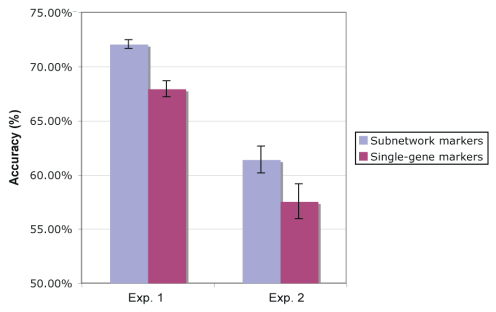
\includegraphics[width=\columnwidth]{figures/Chuang2007figS1.png}
				\caption{Avantages de l'intégration de données d'expression des gènes et d'interactions protéine-protéine sur la précision de la classification de la rechute métastatique par rapport à une analyse classique sur des données d'expression des gènes.}
				\label{fig:Chuang2007figS1}
				\caption*{Figure inspirée de \citeauthor{Chuang2007}.}
			\end{figure}

			\pagebreak

		\subsection{\textcolor{green!45!black}{L'intégration de données d'expression des gènes et d'interactions protéine-protéine}}
			\mylettrine{C}{omme nous venons} de le détailler, cette méthode présente des avantages comparé aux méthodes classiques d'analyse de données d'expression des gènes.
			Nous allons détailler rapidement ici la méthode de \citeauthor{Chuang2007}.
			Cette méthode d'intégration utilise deux types de données.
			Le premier type est les données d'expression des gènes, ainsi que les données cliniques correspondantes, que nous détaillerons dans la Section~\ref{sec:GEP}.
			Le second type de données utilisée est les données d'interactions protéine-protéine, que nous nous détaillerons dans la Section~\ref{sec:IPP}.
			Les conditions cliniques des patients (\emph{ie} métastatique ou non-métastatique) permettent de différencier l'expression des gènes constituant les sous-réseaux pour constituer une matrice d'activité.
			Elles sont utilisés pour assigner des ensembles de gènes sur des sous-réseaux.
			Cette matrice d'activité sert à attribuer un score global à chaque sous-réseau, dérivé de l'expression de chacun des gènes le constituant.
			Des sous-réseaux générés par permutation permettent alors de sélectionner les sous-réseaux discrimants.
			Les sous-réseaux ainsi sélectionnés sont utilisés pour identifier les gènes causant la maladie, et la matrice d'activité du sous-réseau est utilisé pour entraîner un classifieur.

			\begin{figure}
				\centering
				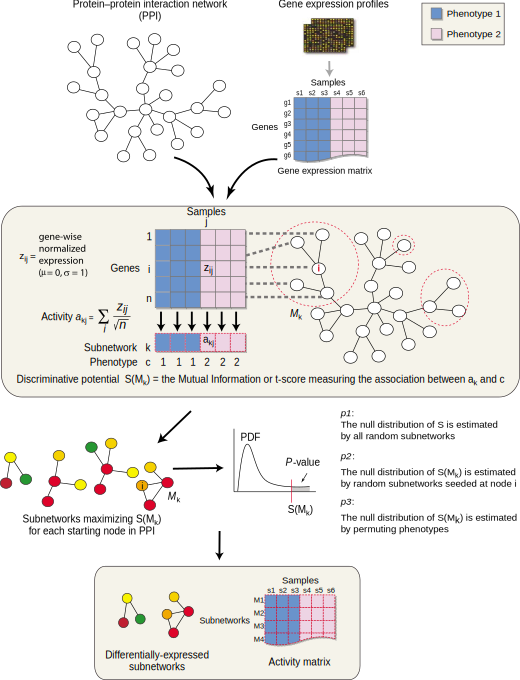
\includegraphics[width=\columnwidth]{figures/Chuang2007IntegrationAlgorithm.png}
				\caption{Algorithme détaillant l'intégration de données d'expression des gènes et d'interactions protéine-protéine.}
				\label{fig:Chuang2007IntegrationAlgorithm}
				\caption*{Figure inspirée de \citeauthor{Chuang2007}.}
			\end{figure}
		
	\section{\textcolor{green!45!black}{L'Intégration Transcriptome-Interactome}}

		\subsection{\textcolor{green!45!black}{L'intégration massive de données d'expression des gènes et de données d'interactions protéine-protéine}}

			\mylettrine{L'}{intégration massive de données} d'expression des gènes et de données d'interactions protéine-protéine est la solution que nous avons développé pour circonvenir aux inconvénients des approches classiques des méthodes de prédiction de la rechute métastatique dans le cancer du sein.

			Nous avons vu précédemment que les approches classiques manquaient de reproductibilité, dépendaient grandement des jeux d'apprentissage et étaient moins performantes utilisées sur un jeu de données indépendant.

			Notre approche est une réimplémentation totale de l'algorithme développé par \citeauthor{Chuang2007}, avec la capacité supplémentaire de pouvoir prendre en compte plusieurs jeux de données d'expression des gènes pour réduire l'effet du fléau de la dimension par l'augmentation du nombre d'échantillons utilisés.

			Nous allons d'abord détailler les données que nous avons utilisées tout au long de ces travaux.
			Ensuite, nous détaillerons l'algorithme.

	\section{\textcolor{green!45!black}{Données transcriptome}}\label{sec:GEP}

		\subsection{\textcolor{green!45!black}{Constitution d'un compendium de données transcriptome dans le cancer du sein}}
			\mylettrine{P}{our constituer un compendium} de données d'expression, nous avons exploré les sites de dépôts de données publiques, ainsi que la littérature, et avons sélectionné les jeux de données dont les conditions cliniques étaient disponibles.
			Nous avons téléchargé l'ensemble des jeux de données sur le dépôt du Gene Expression Omnibus (REF), ou sur le site dédié de l'auteur. Si cela était possible nous avons téléchargé les données brutes, et avons réalisé une normalisation gcrma (package affy du package Bioconductor) sous R.

			\begin{table}
				\begin{center}
					\caption{Liste des jeux de données inclus dans notre compendium de données d'expression dans le cancer du sein.}
					\begin{tabular}{llccc}
						\toprule
						\multirow{3}{3cm}{\emph{Jeu de données}} & \multirow{3}{2cm}{\emph{Plateforme}} & \multirow{3}{2cm}{\centering\emph{Nombre d'échantillons}} & \multirow{3}{2cm}{\centering\emph{Présence de données cliniques}} \\
										&									&		&		\\
										&									&		&		\\
						\midrule
						Anders			& U95v2								& 78	& Non	\\
						Bild			& U95v2								& 158	& Non	\\
						Campone			& UMGC-IRCNA 9k A					& 150	& Non	\\
						Chang			& cDNA array						& 50	& Non	\\
						Chang-Kyu		& Merck GEL Breast Tumor Profiles	& 311	& Non	\\
						Chanrion		& MLRG Human 21K V12.0				& 155	& Non	\\
						Desmedt			& U133A								& 198	& Oui	\\
						Ivshina			& U133 Plus 2.0						& 289	& Oui	\\
						Jezequel		& UMGC-IRCNA 9k A					& 252	& Non	\\
						Kreike			& NKI-AVL 18K cDNA					& 59	& Oui	\\
						Loi				& U133A + U133B						& 327	& Oui	\\
										& U133 Plus 2.0						& 87	& Oui	\\
						Miller			& U133A + U133B						& 251	& Oui	\\
						Parker			& Agilent-011521 1A G4110A			& 2		& Oui	\\
										& Agilent-012097 1A G4110B			& 27	& Oui	\\
										& Agilent 1A Oligo UNC Custom		& 196	& Oui	\\
						Pawitan			& U133A + U133B						& 159	& Oui	\\
						Perou			& SCV								& 84	& Non	\\
						Sabatier		& U133 Plus 2.0						& 129	& Oui	\\
						Schmidt			& U133A								& 200	& Oui	\\
						S{\o}rlie		&									& 85	& Non	\\
						Sotiriou		& U133A								& 189	& Oui	\\
						van de Vijver	& Agilent whole human genome		& 295	& Oui	\\
						van't Veer		& Agilent whole human genome		& 117	& Oui	\\
						Wang			& U133A								& 286	& Oui	\\
						Wong			& U133A								& 6		& Non	\\
						Yu				& U133A								& 341	& Non	\\
						Zhang			& U133A								& 136	& Oui	\\
						Zhou			& U133Av2							& 54	& Oui	\\
						\midrule
						Total			& 7 différentes						& 2572	&		\\
						\bottomrule
					\end{tabular}
					\label{tab:MetDatasets}
					\vspace{3ex}
					\caption*{Tous les jeux de données présentés ici ont été considérés, cependant nous avons gardé seulement les jeux de données accompagnés de données cliniques. Les jeux de données rejetés pourraient cependant être inclus si les données cliniques étaient accessibles.}
				\end{center}
			\end{table}

			Nous avons utilisé ces jeux de données d'expression dans le cancer du sein pour deux analyses.
			Pour la première analyse, non supervisée, nous avons uniquement utilisé comme données cliniques l'événement \acs{DMFS}.
			Voici les jeux de données que nous avons sélectionnés pour notre première analyse (cf Section~\ref{chap:results1}).

			\begin{table}
				\begin{center}
					\caption{Liste des jeux de données inclus pour notre analyse non supervisée (cf Section~\ref{chap:results1}).}
					\begin{tabular}{lcccc}
						\toprule
						\multirow{2}{3cm}{\emph{Jeu de données}}	&  & \multirow{2}{3cm}{\centering\emph{Nombre d'échantillons}}	& \multirow{2}{3cm}{\centering\emph{Nombre de statuts \acs{DMFS} positif}} & \multirow{2}{3cm}{\centering\emph{Nombre de statuts \acs{DMFS} négatif}} \\
						&&&&\\
						\midrule
						Desmedt			& \citep{Desmedt2008}		& 198	& 62	&	136		\\
						Ivshina			& \citep{Ivshina2006}		& 249	& 89	&	160		\\
						Loi				& \citep{Loi2008}			& 117	& 26	&	91		\\
						Parker			& \citep{Parker2009}		& 199	& 45	&	154		\\
						Pawitan			& \citep{Pawitan2005}		& 159	& 40	&	119		\\
						Schmidt			& \citep{Schmidt2008}		& 200	& 46	&	154		\\
						Sabatier		& \citep{Sabatier2011}		& 31	& 9		&	22		\\
						Sotiriou		& \citep{Sotiriou2009}		& 179	& 40	&	139		\\
						van de Vijver	& \citep{vandevijver2002}	& 295	& 88	&	207		\\
						Wang			& \citep{Wang2005}			& 286	& 107	&	179		\\
						Zhang			& \citep{Zhang2009a}		& 136	& 20	&	116		\\
						Zhou			& \citep{Zhou2007}			& 54	& 9		&	45		\\
						\midrule
						Total			&							& 2103	& 581	&	1522	\\
						\bottomrule
					\end{tabular}
					\label{tab:Met:DSNS}
					\vspace{3ex}
					\caption*{L'utilisation de 12 jeux données nous donne l'accès à plus de 2000 tumeurs pour notre analyse non supervisée.}
				\end{center}
			\end{table}

			%Toutes les informations cliniques ont été téléchargés sur \acs{GEO} le site de dépôt de bases de données publiques du \acs{NCBI}, pour les jeux de données préalablement récupérés sur ce même site \citet{Desmedt2008, Loi2008, Sabatier2011, Schmidt2008, Wang2005}, ou sur le site internet de l'auteur\footnote{\url{bioinformatics.nki.nl/data.php}} pour le jeu de données de van de Vijver \citet{vandevijver2002}.

			\pagebreak

			Pour notre seconde analyse, supervisée, nous avons choisi de ne sélectionner que les patientes sans traitement supplémentaire par soucis d'homogénéisation, et ainsi éviter de séparer les patientes en fonction de la réponse au traitement.
			Nous avons également tenu compte de l'expression des \aclp{ER}.
			Dans le but d'avoir un ensemble d'échantillons le plus homogène possible, nous les avons soigneusement choisi en nous basant sur les données cliniques accessibles.
			Les données cliniques qui nous intéressaient, étaient :
			\begin{itemize}
				\item Le statuts \acs{DMFS}
				\item Le temps de mesure de ce statuts \acs{DMFS}
				\item Le statuts \acs{ER}
				\item La présence ou non de traitement, et sa nature éventuelle
			\end{itemize}

			Le statuts \acs{ER} nous a permis de diviser les échantillons en deux groupes pour nos analyses.
			Nous avons utilisé le statuts \acs{DMFS} et son temps de mesure, pour contrôler les échantillons et vérifier qu'il n'y avait pas eu des erreurs d'annotations.
			Les informations sur le traitement nous a permis de sélectionner uniquement les patientes sans traitement supplémentaire.

			\begin{table}
				\begin{center}
					\caption{Liste des jeux de données inclus pour notre analyse supervisée (cf Section~\ref{chap:results2}).}
					\begin{tabular}{llr@{/}lr@{/}lr@{/}l}
						\toprule
						\emph{Jeu de données} & \emph{Plateforme}	& \multicolumn{2}{c}{\emph{Nombre d'échantillons}}	& \multicolumn{2}{c}{\emph{Statuts DMFS}} & \multicolumn{2}{c}{\emph{Statuts ER}} \\
						\cmidrule(r){3-8}
						&  & \emph{(Sélectionnés} & \emph{Total)}	& \emph{(meta} & \emph{non meta)} & \emph{(ER-}	& \emph{ER+)} \\
						\midrule
						Desmedt						& U133A												& 190	&198	& 62	& 128	& 61	& 129	\\
						Loi							& U133A + U133B										& 101	&327	& 27	& 74	& 29	& 72	\\
						Sabatier					& U133 Plus 2.0										& 31	&255	& 9		& 22	& 11	& 20	\\
						Schmidt						& U133A												& 182	&200	& 46	& 136	& 37	& 145	\\
						van de Vijver				& \multirow{2}{2.49cm}{Agilent whole human genome}	& 150	&295	& 56	& 94	& 36	& 114	\\
						& \\
						Wang						& U133A												& 276	&286	& 107	& 169	& 72	& 204	\\
						\midrule
						Total						& 7 différentes										& 930	&1561	& 307	& 623	& 246	& 684	\\
						\bottomrule
					\end{tabular}\label{tab:Met:DSS}
					\vspace{3ex}
					\caption*{L'utilisation de 6 jeux de données nous donne l'accès à plus de 1500 tumeurs pour notre analyse supervisée.}
				\end{center}
			\end{table}

			Après avoir détaillé les jeux de données, leur constitutions, nous allons étudier les interactions protéine-protéine.

	\section{\textcolor{green!45!black}{Interactions protéine-protéine}}\label{sec:IPP}

		\subsection{\textcolor{green!45!black}{Assemblage d'interactomes humains}}
			\mylettrine{L}{a biologie moléculaire} décrit les différents constituants de la cellule (protéines, \acs{ADN}, \acs{ARN} et autres molécules). Mais un organisme vivant est une entité complexe, et il est difficile de le comprendre totalement en analysant des parties spécifiques. C'est pour cela que l'on envisage l'organisme comme un système ou un réseau d'interactions.
			Les protéines interagissent les unes avec les autres dans une cellule, et ces interactions donnent lieu à des fonctions biologiques et un comportement dynamique du système cellulaire. Généralement ces interactions protéine-protéine sont temporelles, spatiales, ou dépendantes d'une condition spécifique.
			L'un des plus grands enjeux dans l'ère post-génomique de la biologie est de récolter des informations d'interactions entre protéines, \acsp{ADN} et autres petites molécules, et de comprendre comment ces interactions sont organisées.
			Les techniques à haut débit ont permis la génération d'un grand nombre de données d'interactions protéine-protéine.
			Pour \acs{ITIfr} nous avons récupéré différentes bases de données d'interactions protéine-protéine.

		\subsection{\textcolor{green!45!black}{Nature des interactions et bases de données d'interactions utilisées}}
			\mylettrine{L}{es interactions contenues} dans les bases de données d'interactions protéine-protéine sont récoltés par différentes techniques, et sont également de différente nature.
			Nous considérons comme sûres les interactions décrites dans la littérature et celle vérifiées par une technique de double hybride dans la levure.
			Les interactions de complexes par co-immuno-précipitation ne sont pas directes, mais concernent des protéines qui font parties d'un même complexe.
			Enfin, les interactions \emph{in silico} sont des prédictions obtenues par divers algorithmes, et ne sont pas validées \emph{in vivo} ou \emph{in vitro}.
			Elles sont donc moins sûres que les autres interactions. 

\pagebreak

			\ac{HPRD} \citep{Prasad2009}, INTAct \citep{Kerrien2012}, \ac{DIP} \citep{Xenarios2000} et \ac{MINT} \citep{Zanzoni2002} contiennent des interactions décrites dans la littérature et vérifiées par double hybride.
			\ac{CORUM} \citep{Ruepp2008} contient des interactions de complexes.
			Cocite \citep{Ramani2005} contient des interactions prédites \emph{in silico}.

	\section{\textcolor{green!45!black}{Données et outils supplémentaires}}\label{sec:outils}
		\mylettrine{N}{ous utilisons} également des données supplémentaires pour les besoins de notre algorithme.
			Pour l'annotation des différentes plateformes de puces à \acs{ADN}, nous utilisons les fichiers fournis par la plateforme d'annotation de puces à \acs{ADN} Resourcerer \citep{Tsai2001}.
			Pour l'annotation des gènes, nous utilisons le fichier gene info \footnote{Homo\_sapiens.gene\_info.gz} fourni par le \acs{NCBI}\footnote{\url{ftp://ftp.ncbi.nlm.nih.gov/gene/DATA/GENE_INFO/Mammalia/}}.

			Nous avons également utilisé des outils supplémentaires pour la visualisation et les analyses de nos résultats.
			Pour visualiser nos sous-réseaux, nous avons utilisé le logiciel libre \emph{Graphviz}\footnote{\url{http://graphviz.org/}} développé par AT\&T Labs Research \citep{Graphviz1988} et le modèle de rendu \emph{neato}.
			Pour analyser l'enrichissement en termes \acs{GO}, nous avons utilisé le programme ErmineJ \citep{Gillis2010}.
			Pour notre analyse supervisée (cf Section ~\ref{chap:results2}) nous utilisons la librarie libSVM \citep{Chang2007} pour classifier nos échantillons (cf Section~\ref{sub:classification}).

	\section{\textcolor{green!45!black}{Présentation de l'algorithme ITI}}\label{sec:ITI}

		\subsection{\textcolor{green!45!black}{Détection des sous-réseaux}}\label{sub:détection}
			\mylettrine{L}{a première étape} de notre algorithme est la détection de sous-réseaux.
			Les données utilisées par \acs{ITIfr} en entrée sont d'une part des profils d'expressions des gènes, ainsi que les conditions cliniques correspondantes aux patients, et des données d'interactions protéine-protéine, détaillés précédemment (données d'expressions des gènes cf Section~\ref{sec:GEP}, données d'interactions protéine-protéine cf Section~\ref{sec:IPP}).
			Les données d'interactions protéine-protéine sont rassemblées pour ne former qu'un seul interactome.
			Les auto-interactions (une protéine vers elle) même n'ont pas été gardées.
			Nous avons gardés les interactions en nous basant sur l'unicité du numéro d'accession gene ID fourni par les fichiers d'annotations du NCBI. 
			Les données d'expressions des gènes sont considérées séparément pour chacun des jeux de données utilisés.
			Chaque gène est utilisé successivement comme graine pour créer un sous-réseau.
			Pour accélérer cette étape de détection des sous-réseaux et minimiser les coûts de calcul, ce processus est parallélisé en subdivisant l'interactome, lors de la sélection des graines, sur un cluster de calcul de type Beowulf.
			Pour chacun des jeux de données d'expression des gènes, la corrélation des conditions cliniques avec les \acs{GEP} est calculé.
			Ainsi, si un gène n'a pas d'expression dans un jeu de données particulier, à cause des différences entre les plateformes, il peut quand même être pris en compte pour la constitution d'un sous-réseaux.
			Récursivement nous considérons le premier voisin du gène graine, et l'ajoutons à notre sous-réseau en construction, si l'ajout de ce gène améliore le score du sous-réseau, suivant l'Équation~\ref{eq:score} :
				\begin{equation}\label{eq:score}
					S_{s,d}=\frac{\sqrt{n_{d}}}{\sqrt{\max n_{d}(DS)}}\Bigg|corr\Bigg(\frac{1}{n}\sum_{g\in S}e(g,d),cc(d)\Bigg)\Bigg|
				\end{equation}
			$S_{s,d}$ est le score du sous-réseau $s$ calculé sur le jeu de données $d$.
			$d$ est un des jeux de données du compendium $DS$, de taille $NS$.
			$corr$ est la corrélation de Pearson mesurée entre la moyenne de l'expression des gènes $e(g,d)$ contenus dans le sous-réseau $s$ et le vecteur $cc$ contenant les conditions cliniques des patients du jeux de données $d$.
			Le score est pondéré par la racine carrée du nombre d'échantillons $nd$ du jeu de données $d$ divisé par le nombre maximum d'échantillons des jeux de données de $DS$.
	
			Le nombre de gènes ajoutés au sous-réseau influence la corrélation entre la moyenne de l'expression des gènes du sous-réseau et les conditions cliniques, et donc le score du sous-réseau.

\pagebreak

			Au plus des sous-réseaux sont ajoutés, au moins l'apport d'un nouveau gène au sous-réseau influencera la valeur du score.
			C'est pourquoi une valeur de seuil nous sert ici pour sélectionner les gènes à ajouter, et ainsi éviter d'ajouter à chaque sous-réseaux la totalité des gènes de l'interactome.

			Un score global, non utilisé pour le calcul, mais pour simplifier l'affichage des résultats est calculé suivant l'Équation~\ref{eq:global} :
			\begin{equation}\label{eq:global}
				S_{s}=\frac{1}{NS}\sum_{d\in DS}S(s,d)
			\end{equation}

			\begin{figure}
				\begin{center}
					\def\svgwidth{\columnwidth}\input{figures/Algorithme.pdf_tex}
					\caption{Principe de la sélection des sous-réseaux avec \acl{ITIfr}.}
					\label{fig:Algorithme}
				\end{center}
			\end{figure}
			$S_{s}$ est le score global du sous-réseau $s$.
			La moyenne des scores est calculé en sommant pour chaque jeu de données $s$ du compendium $DS$, le score $S_{s,d}$ du sous-réseau $s$ sur le jeu de données $s$
			Et en divisant cette somme par $NS$, le nombre de jeux de données dans le compendium $DS$.
		
			Reprenant cette méthode de construction des sous-réseau lors de cette détection, nous construisons, dans le but de valider statistiquement les sous-réseaux que nous venons de détecter, des distributions aléatoires de sous-réseaux.

		\subsection{\textcolor{green!45!black}{Validation statistique}}\label{sec:Validation}
			\mylettrine{D}{ans le but de définir} des distributions aléatoires de scores, nous permettant de vérifier l'hypothèse nulle, reliant l'expression des gènes et les réseaux d'interactions, nous utilisons trois méthodes pour générer des sous-réseaux aléatoires
			Ces méthodes se basent sur le principe de construction de sous-réseaux expliqué précédemment.
			Premièrement, nous mélangeons les conditions cliniques.
			Secondement, la décision d'ajout d'un gène à un sous-réseau ne dépend plus de la corrélation des conditions cliniques avec les \acs{GEP}, mais est aléatoire.
			Troisièmement, nous mélangeons nos interactions protéines-protéines.
			
			Ces trois méthodes différentes nous permettent de générer trois distributions aléatoires de scores qui vont servir pour valider statistiquement les véritables sous-réseaux détectés précédemment.
			Pour garder les ensembles des sous-réseaux aléatoires comparables avec les sous-réseaux détectés, les distributions de leurs tailles sont forcés pour correspondre à celle des sous-réseaux détectés par modèle gaussien.
			Les distributions des scores des sous-réseaux aléatoires sont modélisés par mixture de deux distributions gaussiennes.
			Ces distributions sont utiliser pour fixer des seuils sur les scores, indépendamment des jeux de donnés d'expression, et ainsi leurs attribuer des p-values.
			Le mélange des interactions protéine-protéines ne permet pas de générer un nombre important de sous-réseaux, confirmant l'importance du lien entre les interactions protéines-protéines et le niveau d'expression des gènes.
			La validation statistique est réalisée avec Matlab Statistical Toolbox R2010b.

			\begin{figure}
				\begin{center}
					\def\svgwidth{\columnwidth}\input{figures/DistributionScore.pdf_tex}
					\caption{Distribution des scores des sous-réseaux pour le jeu de données Desmedt.}
					\caption*{Histogramme rouge : distribution aléatoire de sous-réseaux. Courbe bleue : distribution normale (moyenne = 0,0669, $\sigma$ = 0,0777. Histogramme bleu : distribution réelle des sous-réseaux (en A l'ensemble des sous-réseaux avant filtrage, en B les sous-réseaux obtenus après filtrage).}
					\label{fig:Distribution}
				\end{center}
			\end{figure}

		\subsection{\textcolor{green!45!black}{Sélection de sous-réseaux}}\label{sub:Selection}
			\mylettrine{L}{es p-values calculées} lors de l'étape de validation statistique sont utilisées pour filtrer les sous-réseaux détectés statistiquement significatifs.
			Les distributions des trois ensembles de sous-réseaux aléatoires nous ont permis d'attribuer 3 p-values différentes pour chacun des sous-réseaux.
			Nous sélectionnons un seuil de p-value pour chacune des distributions aléatoires et l'utilisons pour filtrer les sous-réseaux détectés et générons trois ensembles de sous-réseaux statistiquement significatifs suivant chacune des méthodes précédemment expliquées.
			Nous réalisons alors l'intersection de ces trois ensemble pour constituer un ensemble de sous-réseaux dont la significativité est validé par trois distributions aléatoires.
			Pour faciliter l'affichage et l'interprétation des résultats, nous combinons les trois différentes p-values avec la méthode de Fisher \citep{Fisher1925}.
			Cet ensemble final de sous-réseaux constitue une signature avec laquelle nous pourrons classifier des échantillons et ainsi comparer la performance des signatures trouvées avec notre méthode ITI et les autres méthodes existantes.
			Nous détaillerons ces résultats dans la Section~\ref{chap:results2}.
			Nous allons maintenant détailler la réalisation d'une ressource bioinformatique contenant les différents sous-réseaux trouvés lors de nos analyses.

		\subsection{\textcolor{green!45!black}{Création d'une ressource bioinformatique permettant l'analyse des sous-réseaux et la reproductibilité de la recherche}}\label{sec:Ressource}
			\mylettrine{P}{our permettre le parcours} des différents ensembles de sous-réseaux trouvés lors de nos analyses, nous avons créé une ressource bioinformatique permettant, l'affichage, l'interprétation et l'analyse des sous-réseaux.
			Cette ressource est accessible par internet, et constitue le site internet compagnon des publications \footnote{\url{http://iti.sourceforge.net/}}.
			Dans un soucis de reproductibilité des résultats, le code source du projet \ac{ITIfr} est disponible sous licence CeCILL sur sourceforge \footnote{\url{http://sourceforge.net/projects/iti/}}.
			L'algorithme ITI nécessitant un cluster de calcul de type Beowulf pour fonctionner, nous avons choisi de l'intégrer à Mobyle, portail permettant de réaliser des analyses bioinformatique.
			Cette intégration permettra de faciliter l'usage d'ITI.
			De plus, les dépendances d'ITI à d'autre outils, comme Matlab nécessitant une licence propriétaire payante, ou ermineJ et Resourcerer, vont être remplacés par des scripts R ou perl, ce qui simplifiera à la fois le pipeline et son déploiement sur d'autres machines.

			Les résultats de chaque analyse sont présents sur cette ressource bioinformatique.
			Pour chaque analyse nous avons accès aux sous-réseaux détectés statistiquement significatifs.
			Une page présente chacun des sous-réseaux.
			Nous avons utilisé le modèle de rendu neato du logiciel GraphViz pour permettre l'affichage des sous-réseaux.
			Une image en format png est générée par jeux de données d'expression pour chacun des sous-réseaux.
			Les scores et les p-values du sous-réseau en fonction du jeu de données d'expression permet de vérifier la significativité des sous-réseaux.
			Pour chacun des gènes du sous-réseau se trouve la valeur de la corrélation des conditions cliniques avec son expression pour chacun des jeux de données d'expression.
			Pour chacun des gènes, un lien vers la page du gène sur le site du NCBI est fournie, pour une analyse plus détaillée.
			Pour permettre plus facilement la navigation d'un sous-réseau à un autre, pour chaque gène il existe une page listant les sous-réseaux dans lesquels il apparaît.

\pagebreak

			Enfin, pour chacun des sous-réseaux un enrichissement en termes \acs{GO} est calculé, par jeux de données d'expression, se basant sur l'apport des gènes du sous-réseaux par rapport à l'ensemble des gènes présents sur la plateforme de puce à \acs{DNA} utilisée pour constituer le jeu de données.

		\subsection{\textcolor{green!45!black}{Utilisation des SVMs pour la classification}}\label{sub:classification}

			\mylettrine{L}{es \acp{SVM}}, ou Séparateurs à Vaste Marge, généralisation des classifieurs linéaires, sont un ensemble de techniques d'apprentissage supervisé destinées à résoudre des problèmes de discrimination et de régression.
			Ils reposent sur deux idées clés : la notion de marge maximale et la notion de fonction noyau.
			La marge est la distance entre la frontière de séparation et les échantillons les plus proches, appelés vecteurs de support.
			La frontière de séparation est choisie comme celle qui maximise la marge et ainsi minimise la capacité (complexité de la classification).
			Pour trouver cette frontière séparatrice optimale, à partir d'un ensemble d'apprentissage, le problème est reformulé comme un problème d'optimisation quadratique, pour lequel des solutions existent déjà.

			La deuxième idée clé est la fonction noyau.
			Pour résoudre les problèmes de discrimination non-linéaire, l'espace de représentation des données d'entrées est transformé en un espace de plus grande dimension (potentiellement infinie), dans lequel il est probable qu'il existe une séparatrice linéaire.
			Une fonction noyau permet de réaliser cela, et a l'avantage de ne pas nécessiter la connaissance explicite de la transformation à appliquer pour le changement d'espace.
			Elle permet d'éviter la transformation coûteuse d'un produit scalaire dans un espace de grande dimension, en une simple évaluation ponctuelle d'une fonction.

			Les \acp{SVM} permettent de traiter des problèmes de discrimination non-linéaire et sont capables de gérer des données de grandes dimensions, c'est pourquoi nous les utilisons pour classifier nos échantillons.

		\subsection{\textcolor{green!45!black}{Stratification, organisation des données et classification}}\label{sub:stratification}
			\mylettrine{P}{our les besoins de notre analyse supervisée} (cf Section~\ref{chap:results2}), nous avons laissé de coté un jeu de données d'expression, dans le but d'effectuer une classification finale indépendante.
			Avec les autres jeux de données d'expression, nous avons réalisé une stratification à dix couches, utilisant 90\% des données pour apprentissage, et les 10\% restant pour classification.

			Nous avons effectué notre stratification en sélectionnant les échantillons de manière à respecter la même proportion entre les différentes couches en échantillons des différents éléments des populations (événement \acs{DMFS} négatif ou positif avec un statuts ER+ ou un statuts ER-).
			
			Nous avons utilisé notre algorithme ITI pour sélectionner des sous-réseaux sur chacune de ces dix couches.
			Nous utilisons la librarie libSVM pour créer des modèles \ac{SVM} pour chacun des jeux de données d'expression utilisés (cf Section~\ref{sub:classification}).
			Chaque liste de sous-réseaux sélectionnée après validation statistique a été utilisée pour trouver la taille maximisant les performances de la classification.
			Pour combiner les différents modèles \ac{SVM}, nous avons réalisé un vote à la majorité pondéré par la taille de la population du jeux de données.

			Chacun de ces ensembles de sous-réseaux a été utilisé pour classifier les 10\% restant.
			Ces dix classifications nous ont permis d'arriver à un ensemble de sous-réseaux optimaux que nous avons alors regroupés.
			Chacun des sous-réseaux a été comparé avec les autres, et s'il y avait une superposition entre deux jeux de données, seul celui avec le meilleur score était gardé.
			Ce dernier ensemble de sous-réseaux a finalement été utilisé pour classifier le jeu de donnés d'expression préalablement mis de coté, et donc indépendant.
			La Figure~\ref{fig:Workflow} détaille cette organisation des données.
			Les résultats seront exploités dans la Section~\ref{chap:results2}.

			\begin{figure}
				\begin{center}
					\def\svgwidth{\columnwidth}\input{figures/Workflow.pdf_tex}
					\caption{Workflow complet des données.}
					\label{fig:Workflow}
				\end{center}
			\end{figure}

\pagebreak

	\section{\textcolor{green!45!black}{Conclusion}}
		\mylettrine{A}{près avoir détaillé} notre méthode, nous allons maintenant présenter les résultats que nous avons obtenus et publiés \citet{Garcia2011,Garcia2012}. Tout d'abord, nous allons détailler nos résultats sur une analyse non-supervisée (cf Section~\ref{chap:results1}), puis sur une analyse supervisée (cf Section~\ref{chap:results2}).
\clearemptydoublepage

% Got papers? great!
\singlespacing

\mychapter{mygreen}{Analyse non-supervisée}
  \sectiongreen*{Résumé}
    \begin{center}
      \begin{tabular}{c}
        \fcolorbox{mydarkgreen}{mylightgreen}{
        \begin{minipage}[][4cm][c]{0.8\linewidth}
          \sffamily
            \ref{app:Garcia2011}
        \end{minipage}}\\
        \\[2ex]
        \begin{minipage}[][4cm][c]{0.9\linewidth}
          \mtcsetdepth{minitoc}{1}
          \minitoc
        \end{minipage}
      \end{tabular}
    \end{center}
    \newpage

\doublespacing

	\section{\textcolor{mygreen}{Détails de l'analyse non-supervisée}}
    \subsection{\textcolor{mygreen}{Organisation des études}}
    Quatre études différentes on été réalisées
        \begin{table}
        \begin{center}
          \caption{Organisation de la validation croisée}
          \begin{tabular}{ll}
            \toprule
            \emph{Étude} & \emph{Jeu de données d'entraînement} \\
            \midrule
            A1 &  Tous sauf van de Vijver                       \\
            B1 &  Tous sauf Wang                                \\
            A2 &  Tous ceux sur plateforme Affymetrix           \\
            B2 &  Tous ceux sur plateforme Affymetrix sauf Wang \\
            \bottomrule
          \end{tabular}
          \label{tab:Res1Train}
          \vspace{5ex}
          \caption*{Deux études sont réalisés à partir de tous les jeux de données de notre compendium sauf un (A1, B1), tandis que deux autres études sont réalisés à partir des jeux de données profilés sur plateforme Affymetrix pour comparer les performances de notre algorithme entre différentes plateformes.}
        \end{center}
      \end{table}

	\section{\textcolor{mygreen}{Performances}}
	\section{\textcolor{mygreen}{Exploration des sous-réseaux}}
  \section{\textcolor{mygreen}{{Conclusion}}}
\clearemptydoublepage

% Got papers? great!
\singlespacing

\mychapter{green!45!black}{Analyse supervisée}\label{chap:results2}
	\sectiongreen*{Résumé}
		\begin{center}
			\begin{tcolorbox}[colback=green!5!white,colframe=green!45!black,arc=0mm]
				\sffamily
				Dans ce chapitre nous allons présenter les résultats que nous avons obtenus lors de l'utilisation d'ITI sur une analyse supervisée.
				Ces résultats sont détaillés dans notre article \emph{Interactome–transcriptome integration} \citet{Garcia2012} présent dans les Annexes~\ref{app:Garcia2012} de cet ouvrage.
			\end{tcolorbox}
			\vspace{5ex}
			\mtcsetdepth{minitoc}{1}
			\minitoc
		\end{center}
		\newpage

\doublespacing

	\section{\textcolor{green!45!black}{Détails de l'analyse supervisée}}
		\subsection{\textcolor{green!45!black}{Organisation des jeux de données transcriptome en deux études}}
		\mylettrine{N}{ous avons organisé} notre analyse supervisée en deux études.
		Ces deux études se basent sur le même compendium de donnés transcriptomique (cf Tableau~\ref{tab:Met:DSS}), en mettant de coté, pour validation indépendante, un jeu de données différent à chaque fois (Desmedt ou van de Vijver, cf Tableau~\ref{tab:Res2Data}).
		Pour chacune de ces deux études nous avons de plus séparé les échantillons suivant leurs statuts \acs{ER} pour permettre une plus grande homogénéité des données.
		Pour éviter un sur-entraînement lors de la détection des sous-réseaux, nous avons organisé une stratification à 10 couches.
		La stratification a été réalisé en conservant entre les différentes populations des couches de la stratification la même proportion en individus, se basant sur les statuts \acs{ER} et les conditions cliniques (cf Section~\ref{sub:stratification}).

		La détection des sous-réseaux a été ensuite réalisée comme présenté dans la Section~\ref{sec:ITI} et a mené à la détection de 165 sous-réseaux (pour les échantillons ER-) et de 6 sous-réseaux (pour les échantillons ER+) pour la première étude, et de 122 sous-réseaux (pour les échantillons ER-) et de 14 sous-réseaux (pour les échantillons ER+) pour la seconde étude.
		Le nombre de sous-réseaux est moins important pour les échantillons ER+, cela reflète une plus grande homogénéité des échantillons.
		Ces résultats sont détaillés dans le Tableau~\ref{tab:Res2pvalue}.

		Nous allons maintenant passer à l'analyse des performances de signatures obtenues avec ces différentes études sur la prédiction de la rechute métastatique.

		\begin{table}
				\begin{center}
					\caption{Liste des jeux de données utilisés dans l'analyse supervisée.}
					\begin{tabular}{llr@{/}lr@{/}lr@{/}l}
						\toprule
						\emph{Jeu de données} & \emph{Plateforme} & \multicolumn{2}{c}{\emph{Nombre d'échantillons}} & \multicolumn{2}{c}{\emph{Statuts DMFS}} & \multicolumn{2}{c}{\emph{Statuts ER}} \\
						\cmidrule(r){3-8}
						&  & \emph{(Sélectionnés} & \emph{Total)}           & \emph{(meta} & \emph{non meta)} & \emph{(ER-}     & \emph{ER+)} \\
						\midrule
						\textbf{Desmedt}          & \textbf{U133A}          & \textbf{190} & \textbf{198} & \textbf{62} & \textbf{128} & \textbf{61} & \textbf{129} \\
						Loi                       & U133A + U133B           & 101 & 327                   & 27 & 74                & 29 & 72            \\
						Sabatier                  & U133 Plus 2.0           & 31 & 255                    & 9 & 22                 & 11 & 20            \\
						Schmidt                   & U133A                   & 182 & 200                   & 46 & 136               & 37 & 145           \\
						\textbf{van de Vijver}    & \multirow{2}{2.49cm}{\textbf{Agilent whole human genome}}  & \textbf{150} & \textbf{295} & \textbf{56} & \textbf{94}  & \textbf{36} & \textbf{114} \\
						& \\
						Wang                      & U133A                   & 276 & 286                   & 107 & 169              & 72 & 204           \\
						\midrule
						Total                     & 7 différentes           & 930 & 1561                  & 307 & 623              & 246 & 684          \\
						\bottomrule
					\end{tabular}\label{tab:Res2Data}
					\vspace{5ex}
					\caption*{Deux études ont été réalisées en utilisant différentes combinaisons pour les jeux de donnés d'entraînement et ceux de validation (\textbf{en gras}). Dans l'étude 1 les échantillons provenant de Desmedt ont été mis de côté pour validation indépendante, et l'entraînement a eu lieu avec les autres jeux de données. Les échantillons provenant de van de Vijver ont été pareillement mis de côté pour validation indépendante dans l'étude 2.}
				\end{center}
			\end{table}
				\begin{table}

				\begin{center}
					\caption{Taille et p-value de la signature retenue pour chacune des études réalisées.}
					\begin{tabular}{ccccc}
						\toprule
						\multirow{2}{2cm}{\centering\emph{Étude}} & \multirow{2}{1.5cm}{\centering\emph{Statuts}} & \multirow{2}{1.5cm}{\centering\emph{seuil de P-value}} & \multirow{2}{2cm}{\centering\emph{Nombre de sous-réseaux}} & \multirow{2}{1.5cm}{\centering\emph{Nombre de gènes}} \\
						&&&&\\
						\midrule
						Étude 1      & ER-            & 1e\textsuperscript{-4}  & 165                           & 2310                    \\
						Étude 1      & ER+            & 1e\textsuperscript{-4}  & 6                             & 175                     \\
						Étude 2      & ER-            & 1e\textsuperscript{-4}  & 122                           & 1481                    \\
						Étude 2      & ER+            & 1e\textsuperscript{-4}  & 14                            & 272                     \\
						\bottomrule
					\end{tabular}
					\label{tab:Res2pvalue}
					\vspace{5ex}
					\caption*{Le nombre optimal de sous-réseaux pour une classification dépend des jeux de données utilisés pour l'apprentissage. Le fait qu'il soit plus faible pour les ER+ reflète une plus grande homogénéité des échantillons.}
				\end{center}
			\end{table}

		\section{\textcolor{green!45!black}{Performances des signatures obtenues sur la prédiction de la rechute métastatique}}
		\mylettrine{D}{eux signatures séparées} ont été générées pour les sous-types ER+ et ER- pour nos deux différentes études.
		Nous avons donc obtenus au final quatre ensembles de sous-réseaux.
		La taille optimale retenue dans le Tableau~\ref{tab:Res2pvalue} est celle qui maximise la précision moyenne sur les dix couches de la stratification pour chacune des études.
		Pour l'étude 1, les sous-réseaux discriminatifs retenus avaient un score moyen de 0.49 (ER+) et 0.54 (ER-) confirmant la haute corrélation entre la co-expression et la proximité dans l'interactome.
		La taille des signatures était respectivement de 6 (ER+) et 165 sous-réseaux (ER-).
		Pour l'étude 2, la signature ER+ avait un score de classification optimal pour 14 sous-réseaux, et la signature ER- pour 122 sous-réseaux.
		Ces sous-réseaux correspondent respectivement à des listes de 175 (Étude 1, ER+), 2310 (Étude 1, ER-), 272 (Étude 2, ER+) et 1481 (Étude 2, ER-) gènes.
		Un grand nombre de gènes étant représentés dans plusieurs sous-réseaux.
		Ces nombre sont plus larges que ceux reporté pour les autres signatures.
		Ceci suggère que nous avons détecté un nombre important de gènes significativement liés à la rechute métastatique, reflétant de façon réaliste à la fois l'empreinte biologique de la métastase et l'ampleur des perturbations au niveau de l'expression des gènes.
		La redondance des gènes dans les sous-réseaux peut être expliquée par la haute connectivité de certains hubs (comme \acs{TP53}), ce qui augmente leur probabilité d'être intégré dans plusieurs sous-réseaux.

		Pour évaluer la performance des signatures découvertes avec ITI, nous les avons comparées avec des signatures déjà établies.
		Les 128 sondes du \acs{GGI} \citep{Sotiriou2006}, la signature Mammaprint à 70 gènes \citep{vandevijver2002} et la signature statuts ER spécifique à 76 gènes \citep{Wang2005} ont été testées.
		La performance a été mesuré sur les mêmes échantillons (jeux de données Desmedt et van de Vijver), séparément sur les tumeurs ER+ et ER-.
		La méthode de classification originale des signatures a été utilisée.
		Pour la signature de van de Vijver, les distances aux centroïdes moyens entre les groupes avec et sans rechute ont été calculées \citep{vandevijver2002}.
		Pour la signature de Wang, un score de rechute est calculé pour chaque patient par combinaison linéaire de l'expression des gènes pondéré par des coefficients de Cox standardisés \citep{Wang2005}.
		Les signature GGI et Mammaprint étant sondes-spécifiques, les tests ont donc été réalisés avec les sondes présentes dans le jeu de données de validation.
		Les résultats et les mesures des performances sont détaillés dans le Tableau~\ref{tab:Res2Classif}.

			\begin{sidewaystable}
				\begin{center}
					\caption{Comparaison des résultats de classification entre ITI et d'autres signatures sur les jeux de données de validation Desmedt et van de Vijver pour les tumeurs ER- et ER+.}
					\begin{tabular}{crrrrrrrrrrrrrrrr}
						\toprule
						\multicolumn{1}{c}{\emph{Statuts}} & \multicolumn{8}{c}{ER-} & \multicolumn{8}{c}{ER+} \\
						\cmidrule(r){2-9}\cmidrule(r){10-17}
						\multicolumn{1}{c}{\emph{Jeux de}} & \multicolumn{4}{c}{\multirow{2}{*}{\emph{Desmedt}}} & \multicolumn{4}{c}{\multirow{2}{*}{\emph{van de Vijver}}} & \multicolumn{4}{c}{\multirow{2}{*}{\emph{Desmedt}}} & \multicolumn{4}{c}{\multirow{2}{*}{\emph{van de Vijver}}} \\
						\multicolumn{1}{c}{\emph{Données}} & & & & \\
						\cmidrule(r){2-5}\cmidrule(r){6-9}\cmidrule(r){10-13}\cmidrule(r){14-17}
						\multirow{2}{*}{\emph{Signature}} & \emph{GGI} & \emph{70g} & \emph{76g} & \multicolumn{1}{c}{\emph{\textbf{ITI}}} & \emph{GGI} & \emph{70g} & \emph{76g} & \multicolumn{1}{c}{\emph{\textbf{ITI}}} & \emph{GGI} & \emph{70g} & \emph{76g} & \multicolumn{1}{c}{\emph{\textbf{ITI}}} & \emph{GGI} & \emph{70g} & \emph{76g} & \multicolumn{1}{c}{\emph{\textbf{ITI}}}    \\
											&     &     &     & \multicolumn{1}{c}{\emph{\textbf{(165)}}}              &     &     &     & \multicolumn{1}{c}{\emph{\textbf{(122)}}}  &     &     &     & \multicolumn{1}{c}{\emph{\textbf{(6)}}}                &     &     &     & \multicolumn{1}{c}{\emph{\textbf{(14)}}}   \\
						\midrule
						N         & 61    & 61    & 61    & \textbf{61}                               & 36    & 36    & 36    & \textbf{36}                   & 129   & 129   & 129   & \textbf{129}                              & 114   & 114   & 114   & \textbf{114}                   \\
						\midrule
						VN        & 6     & 0     & 14    & \textbf{22}                               & 3     & 2     & 12    & \textbf{17}                   & 63    & 28    & 53    & \textbf{86}                               & 57    & 39    & 50    & \textbf{49}                    \\
						FP        & 28    & 34    & 20    & \textbf{12}                               & 16    & 17    & 7     & \textbf{2}                    & 31    & 66    & 41    & \textbf{8}                                & 18    & 36    & 25    & \textbf{26}                    \\
						VP        & 23    & 27    & 9     & \textbf{11}                               & 14    & 17    & 8     & \textbf{2}                    & 21    & 25    & 25    & \textbf{9}                                & 20    & 32    & 22    & \textbf{10}                    \\
						FN        & 4     & 0     & 18    & \textbf{16}                               & 3     & 0     & 9     & \textbf{15}                   & 14    & 10    & 10    & \textbf{26}                               & 19    & 7     & 17    & \textbf{29}                    \\
						\midrule
						ACC       & 0.46  & 0.42  & 0.38  & \textbf{0.54}                             & 0.47  & 0.53  & 0.56  & \textbf{0.53}                 & 0.65  & 0.41  & 0.60  & \textbf{0.74}                             & 0.68  & 0.62  & 0.63  & \textbf{0.52}                  \\
						SV        & 0.85  & \multicolumn{1}{l}{1} & 0.33  & \textbf{0.41}             & 0.82  & \multicolumn{1}{l}{1} & 0.57  & \textbf{0.12} & 0.60  & 0.71  & 0.71  & \textbf{0.26}                             & 0.51  & 0.82  & 0.56  & \textbf{0.26}                  \\
						SP        & 0.18  & \multicolumn{1}{l}{0} & 0.41  & \textbf{0.65}             & 0.16  & 0.11                  & 0.63  & \textbf{0.90} & 0.67  & 0.30  & 0.56  & \textbf{0.92}                             & 0.76  & 0.52  & 0.67  & \textbf{0.65}                  \\
						\bottomrule
					\end{tabular}
					\label{tab:Res2Classif}
					\vspace{5ex}
					\caption*{Les quatre signatures ont été utilisés pour mesurer la performance de classification d'ITI (\textbf{en gras}). Les abréviations suivantes ont été utilisées : N - nombre de tumeurs à classifier; VN - Vrai Négatif; FP - Faux Positif; VP - Vrai Positif; FN - Faux Négatif; ACC - Justesse; SV - Sensibilité; SP - Spécificité. La performance de la classification basée sur les sous-réseaux est supérieure à la classification basée sur l'expression des gènes pour prédire la métastase dans le jeu de données de Desmedt, et ce de façon similaire pour le jeu de données de van de Vijver.}
				\end{center}
			\end{sidewaystable}

		Ces résultats montrent que notre algorithme ITI possède une performance largement plus généralisable que les autres signatures précédemment publiées.
		La classification par le GGI montre une précision maximale entre 47 et 68 \%, la signature à 70 gènes entre 41 et 62 \% et la signature à 76 gènes entre 37 et 63\%.
		ITI a une meilleure précision, comparée à la signature de Wang sur les données de Desmedt (ER+) : une précision de 74\% (spécificité de 92\%) a été obtenue contre une précision de 60\% (spécificité de 56\%) pour la signature à 76 gènes.
		ITI donne aussi des résultats plus performants sur les échantillons ER- des données Desmedt avec une précision de 54\% (spécificité de 65\%) contre une précision de 38\% (spécificité de 41\%) contre la signature de Wang.
		Ceci reste également vrai pour la signature Mammaprint à 70 gènes qui marche essentiellement sur le jeu de données van de Vijver.
		ITI montre une performance de 53\% associée à une spécificité de 90\% sur les données van de Vijver (ER-) et une précision de 52\% avec une spécificité de 65\% sur les données van de Vijver (ER-). 
		Cette performance est inférieure à celle obtenu sur l'étude 1 et pourrait refléter un biais vers les plateformes Affymetrix introduit par l'apprentissage sur le compendium. 
		Le signature Mammaprint est caractérisée par une précision inférieure (41\% sur les tumeurs ER+ et de 42\% sur les tumeurs ER- du jeu de données Desmedt).
		De la même manière, ITI a montré une performance supérieure à la classification GGI sur les patients ER-.
		Globalement, ITI a été capable de mieux généraliser avec valeur minimale pour la précision de 52\%.

		À titre de comparaison, \citet{Chuang2007} ont achevé une performance de 48.8\% sur les échantillons issus du jeu de données van de Vijver en les entraînant sur ceux du jeu de données Wang et 55.8\% réciproquement.
		Les contributions spécifiques des données d'interactions ou des données d'expression des gènes ne sont pas quantifiées, elles sont difficilement séparables dans la configuration actuelle.
		Cependant, \citet{Chuang2007} ont déjà démontré que qu'une approche intégrative augmentait la robustesse de la signature, et plusieurs études ont démontré que des méta-analyses de données d'expression des gènes augmentaient également les performances de classification \citep{Fishel2007,Xu2005}.
		Nous avons réalisé une analyse du temps de survie entre les groupes de bon et mauvais pronostics dans l'étude 1 (cf Figure~\ref{fig:Survival}).
		Un test Log-rank donne une p-value de 4.89x10\textsuperscript{-5}, suggérant une bonne séparation entre les deux groupes.
		Cette valeur est plus élevée que les p-values obtenues avec les autres signatures (la signature de Wang donne P = 4.11x10\textsuperscript{-3} et celle du GGI donne P = 1.34x10\textsuperscript{-3}).
		La signature Mammaprint n'a pas été capable de séparer significativement dans des groupes les patients issus du jeu de données de Desmedt.
		Même si ITI n'a pas été spęcifiquement prévu pour obtenir un bon score au test Log-rank, il a été capable de séparer les patients avec une haute espérance de survie de ceux avec une espérance de survie faible.
		Une alternative aurait pu être de calculer directement les scores des sous-réseaux en se basant sur les P-values du log-rank des gènes.

		\section{\textcolor{green!45!black}{Exploration des sous-réseaux}}

			\mylettrine{D}{ous avons examiné} les enrichissements en termes Gene Ontology pour la catégorie "biological process" pour les sous-réseaux obtenus dans l'étude 1.
			La Table~\ref{tab:Res2GO} montre plusieurs enrichissements en termes \acs{GO} pour les deux signatures ER+ et ER-.
			Les termes \acs{GO} trouvés dans les sous-réseaux discriminatifs sont reliés à des processus regulationnels perturbé dans le cancer (cycle cellulaire, contrôle des dommages à l'ADN) et dans la métastase (système immunitaire, prolifération cellulaire, adhésion focale, migration cellulaire et organisation du cytosquelette) à la fois dans les tumeurs ER+ et dans les ER-. 
			Comme exemple, nous décrivons ici un sous-réseau significativement associé avec la métastase dans l'étude 1 (ER-), le sous-réseau 6693 (cf Figure~\ref{fig:Subnetwork6693}).
			Ce sous-réseau contient des gènes avec des fonctions connues pour leur implication dans les cancers du sein ER- et la métastase, comme le \acs{TSG} \acs{TP53} et les récepteurs \acs{ERBB2} et \acs{EGFR}.
			Ce sous-réseau contient également plusieurs kinases et régulateurs du cycle cellulaire (\acs{CDK2}, \acs{CDKN1A}, \acs{CDKN2A}, \acs{NQO1}), dont l'altération de l'expression a été précédemment associée avec plusieurs types de cancer.
			\acs{PIN1} est présent dans ce sous-réseau et il a été récemment trouvé qu'il promouvait l'agressivité des tumeurs dans le cancer du sein.
			Le récepteur à l'insuline est également présent; la dérégulation de son expression est corrélée avec une mauvaise réponse aux traitements anti-\acs{IGFR} dans les cancers du sein triple négatif.
			Ce sous-réseau contient également de nombreux oncogènes et des gènes non-précédemment reliés au cancer, mais qui pourrait agir comme des gènes directeurs du cancer du sein.

		\begin{table}
				\begin{center}
					\caption{Enrichissement en termes \acs{GO} des sous-réseaux ER- et ER+}
					\begin{tabular}{clccr}
						\toprule
						& \multicolumn{1}{c}{\emph{Terme \acs{GO}}} & \emph{GOID} & \emph{P-value corrigée} \\
						\midrule
						\multirow{5}{*}{\emph{ER-}} & Natural killer cell-mediated imunity                      & GO:0002228  & 293e\textsuperscript{-06} \\
																				& Positive regulation of MAP kinase activity                & GO:0043406  & 476e\textsuperscript{-10} \\
																				& Muscle cell development                                   & GO:0055001  & 106e\textsuperscript{-11} \\
																				& Interphase of mitotic cell cycle                          & GO:0051329  & 408e\textsuperscript{-11} \\
																				& Wnt receptor signaling pathway through ${\beta}$-catenin  & GO:0060070  & 622e\textsuperscript{-10} \\
						\midrule
						\multirow{5}{*}{\emph{ER+}} & mRNA cleavage                                             & GO:0006379  & 125e\textsuperscript{-08} \\
																				& Regulation of growth hormone secretion                    & GO:0060123  & 218e\textsuperscript{-07} \\
																				& Positive regulation of cytoskeleton organization          & GO:0051495  & 206e\textsuperscript{-04} \\
																				& Regulation of insulin secretion                           & GO:0050796  & 155e\textsuperscript{-05} \\
																				& Regulation of chemotaxis                                  & GO:0050920  & 429e\textsuperscript{-07} \\
						\bottomrule
					\end{tabular}
					\label{tab:Res2GO}
					\vspace{5ex}
					\caption*{Plusieurs enrichissements en termes \acs{GO} pour les sous-réseaux extraits dans l'étude 1 (ER- et ER+) sont reliés au cancer.}
				\end{center}
			\end{table}

			\begin{figure}
				\begin{center}
					\def\svgwidth{\columnwidth}\input{figures/Survival.pdf_tex}
					\caption{Comparatif des courbes de survies des patients.}
					\label{fig:Survival}
				\end{center}
			\end{figure}

			\begin{figure}
				\begin{center}
					\def\svgwidth{\columnwidth}\input{figures/Subnetwork6693.pdf_tex}
					\caption{Représentation graphique d'une partie du sous-réseau 6693, Étude 1 ER-.}
					\label{fig:Subnetwork6693}
					\caption*{Ce sous-réseau discriminatif a été découvert sur les données issues de \citet{Sabatier2011}.
					Les n{\oe}uds et les arcs correspondent respectivement aux gènes codant pour des protéines et aux \acs{PPI}.
					Les couleurs jaunes et bleues des n{\oe}uds montrent respectivement une sur-expression et une sous-expression en comparant les patients avec métastases et ceux sans.}
				\end{center}
			\end{figure}


\pagebreak
	\section{\textcolor{green!45!black}{Conclusion}}

	\mylettrine{L'}{analyse} supervisée réalisée avec ITI nous a permis de confirmer la significativité biologique des sous-réseaux découverts.
		La classification indépendantes des échantillons nous a permis de comparer les signatures obtenues avec ITI et les signatures précédemment établies.
		Nous avons donc pu confirmer l'avantage de l'ITI sur la robustesse des performances de la signature ainsi que sa reproductibilité sur un jeu de données indépendant.
		Nous allons maintenant discuter des autres avantages de cette approche.

\clearemptydoublepage

% Make sense of the whole of it
\singlespacing

\mychapter{blue!45!black}{Discussion Générale}
	\sectionblue*{Résumé}
		\begin{center}
			\begin{tcolorbox}[colback=blue!5!white,colframe=blue!45!black,arc=0mm]
				\sffamily
				Après un bref récapitulatif des travaux effectués lors de cette thèse, nous traiterons dans cette conclusion l'importance que peuvent avoir les données initiales et la question biologique posée sur la performance des signatures, la taille des sous-réseaux et la significativité biologique des signatures.
				Nous analyserons ensuite les caractéristiques des signatures obtenues avec ITI en les comparant avec les signatures précédemment citées.
				Nous finirons cette discussion en exposant des perspectives sur l'évolution de l'algorithme et des analyses futures.
			\end{tcolorbox}
			\vspace{5ex}
			\mtcsetdepth{minitoc}{1}
			\minitoc
		\end{center}
		\newpage

\doublespacing

	\section{\textcolor{blue!45!black}{Rappels sur les travaux effectués}}
		\mylettrine{N}{ous avons dans cet ouvrage} exploré les caractéristiques biologiques des cancers et les spécificités du cancer du sein\index{cancer!cancer du sein}.
		Nous avons ensuite montré qu'une perturbation de l'expression et/ou la régulation des gènes pouvait être à l'origine du cancer.
		Nous avons rappelé l'intérêt des approches de médecines personnalisée et prédictive de classifier les tumeurs pour pouvoir les traiter de manière spécifique et proposer une thérapie adaptée.
		Après avoir exposé les limitations de l'approche transcriptomique à haut-débit pour étudier le cancer, nous avons détaillé notre méthode ITI, puis nous avons exposé les résultats d'une analyse non-supervisée et d'une analyse supervisée.

	\section{\textcolor{blue!45!black}{Importance des données initiales}}
		\mylettrine{L}{e jeu de données d'apprentissage} a une grande importance lors de l'établissement d'une signature prédictive, comme l'a montré \citeauthor{Michiels2005}.
		Ce phénomène est dû à la fois à la topologie des données et à la biologie du cancer (cf Section~\ref{def:limitations}).
		Notre approche intégrant simultanément plusieurs jeux de données transcriptome permet de moins dépendre des jeux de données initiaux.
		De plus, le fait d'homogénéiser les échantillons permet de minimiser la variation biologique dûe au cancer.
		Ainsi lors de la détection du sous-réseau, un gène n'ayant pas de variation d'expression dans un jeu de données peut être pris en compte pour la constitution d'un sous-réseaux, si son expression varie suivant les conditions cliniques dans un autre jeu de données (cf Section~\ref{sub:détection}).
		Avec un compendium de plusieurs jeux de données recouvrant 930 tumeurs, nous obtenons une performance de classification supérieure sur un jeu de données totalement indépendant comme nous l'avons montré dans l'exploration des résultats de notre analyse supervisée (cf Table~\ref{tab:Res2Classif}).
		Nous avons comparé les signatures réalisées avec ITI et les signatures issues de la littérature \citep{vandevijver2002,Wang2005,Sotiriou2006}.

	\section{\textcolor{blue!45!black}{Caractéristiques des signatures réalisées}}

		\subsection{\textcolor{blue!45!black}{Amélioration de la stabilité, robustesse et reproductibilité}}
			\mylettrine{P}{our comparer la pertinence} de nos sous-réseaux aux signatures déjà publiées, nous avons récupéré dans les articles originaux, les listes des sondes constituant la signature Mammaprint à 70 gènes \citep{vandevijver2002}, la signature statuts ER spécifique à 76 gènes \citep{Wang2005}, et la signature du \acs{GGI} \citep{Sotiriou2006}. Nous avons utilisé les annotations les plus récentes des sondes, enlevé les doublons, et n'avons pas considéré les EST. Les annotations des sondes étant constamment mises à jour, il peut y avoir une variation sur le nombre de gènes, c'est pourquoi nous trouvons un seul gène commun entre les signatures \citet{vandevijver2002} et \citet{Wang2005} alors que \citet{Chuang2007} en trouvaient 3. C'est également la raison pour laquelle la signature GGI \citep{Sotiriou2006} que nous avons réalisé contient 108 gènes (et non 97 comme précisé dans la littérature).
			La Figure~\ref{fig:Venn} compare les différentes signatures et notamment les gènes en communs.
			\begin{figure}
				\begin{center}
					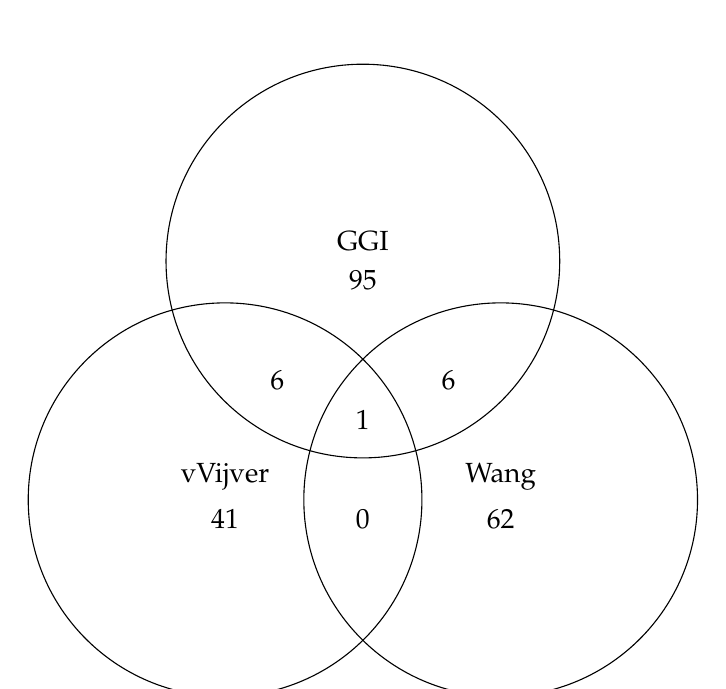
\begin{tikzpicture}
						\tikzset{venn circle/.style={draw,circle,minimum width=5cm}}
						\node [venn circle] (A) at (0,0)								{};
							\node [above]		at (A) 									{vVijver};
							\node [below]		at (A) 									{41};
						\node [venn circle] (B) at (60:3.5cm)							{};
							\node [above]		at (B) 									{GGI};
							\node [below]		at (B) 									{95};
						\node [venn circle] (C) at (0:3.5cm)							{};
							\node [above]		at (C) 									{Wang};
							\node [below]		at (C) 									{62};
							\node [left]		at (barycentric cs:A=1/2,B=1/2)			{6};
							\node [below]		at (barycentric cs:A=1/2,C=1/2)			{0};
							\node [right]		at (barycentric cs:B=1/2,C=1/2)			{6};
						\node					at (barycentric cs:A=1/3,B=1/3,C=1/3)	{1};
					\end{tikzpicture}
				\end{center}
				\caption{Diagramme de Venn comptabilisant les gènes communs entre les différentes signatures classiques.}\label{fig:Venn}
			\end{figure}

			Il apparaît que très peu de gènes sont communs entre ces signatures (moins de 5\% de la totalité des gènes des signatures deux à deux).
			À titre de comparaison, nous avons croisé les deux signatures ITI obtenues sur les échantillons ER+ et ER- avec nos deux études de notre analyse supervisée.
			Un total de 937 gènes sont communs entre nos deux signatures pour les échantillons ER-, et 46 gènes sont communs pour les signatures réalisées sur les échantillons ER+.
			Cela représente un recouvrement de respectivement 32.8\% (ER-) et 11.5\%(ER+).
			Ces valeurs relativement basses reflètent les biais dus aux jeux de données et aux plateformes de puces à ADN.
			Cependant, ce recouvrement est largement supérieur aux quelques gènes communs entre les autres signatures.
			Il pourrait être probablement augmenté en utilisant un ensemble de jeux de données d'entraînement plus large.

		\subsection{\textcolor{blue!45!black}{Significativité biologique relevante}}
			\mylettrine{R}{eprenant les trois signatures établies} dans la littérature (la signature Mammaprint à 70 gènes \citep{vandevijver2002}, la signature statuts ER spécifique à 76 gènes \citep{Wang2005}, et la signature du \acs{GGI} \citep{Sotiriou2006}), \citeauthor{HaibeKains2008} supposent que les pronostics sur le devenir des patients sont basés sur la représentation de processus biologiques qui se recouvrent largement.
			\citeauthor{Thomassen2007} ont comparé 9 signatures pronostiques, et ont trouvé que le cycle cellulaire et la prolifération cellulaire étaient les termes \acs{GO} les plus représentés.
			\citeauthor{Yu2007} ont conduit des analyses sur les différentes voies de régulation de 5 signatures prognostiques publiées avaient un grand nombre de voies en commun, comme le cycle cellulaire, la régulation du cycle cellaire, la mitose, l'apoptose, etc \dots
			\citeauthor{HaibeKains2008} ont étudié dans une méta-analyse à grande échelle des données publiques d'expression des gènes et ont trouvé que la prolifération était une force directrice commune d'un grand nombre de signatures pronostiques.
			Nous retrouvons dans nos analyses ces processus biologiques impliqués dans le cancer et la métastase, mais également d'autres processus, comme le contrôle des dommages à l'ADN et le système immunitaire qui sont également important.

		\subsection{\textcolor{blue!45!black}{Taille des sous-réseaux}}
			\mylettrine{L}{a question biologique} posée a son importance.
			Dans le cadre d'un cancer très hétérogène comme le cancer du sein, un nombre de gènes important est nécessaire pour réaliser une classifieur sur une question complexe comme la rechute métastatique.
			Si la question posée est la différentiation entre deux types de cancer où beaucoup de gènes sont différentiellement exprimés, comme pour la leucémie myéloïde aiguë et la leucémie lymphoblastique aiguë, peu de gènes peuvent suffire pour différencier les deux conditions cliniques \citet{Dobbin2008}.
			L'homogénéité des données a également son rôle dans la taille finale des sous-réseaux, comme nous l'avons vu précédemment.

	\section{\textcolor{blue!45!black}{Création d'une base de donnés de sous-réseaux}}
			\mylettrine{L}{a création d'une ressource} bioinformatique permettant l'exploration des sous-réseaux.
			Cette ressource, a été mise en place, accessible par Internet, contient pour chacune de nos analyses les sous-réseaux détectés statistiquement significatifs.
			Pour chacun des sous-réseaux, un enrichissement en termes \acs{GO} est calculé, par jeux de données d'expression, en se basant sur l'apport des gènes du sous-réseaux par rapport à l'ensemble des gènes présents sur la plateforme de puce à \acs{DNA} utilisée pour constituer le jeu de données.
			Cette ressource permet de relier l'interactome à la biologie de la maladie étudiée, ici dans le cadre du cancer du sein.
			Les sous-réseaux stockés étant discriminatifs pour la rechute métastatique dans le cancer du sein, leur exploration, facilitée par des analyses en enrichissement en termes \acs{GO} permet la découverte de gènes d'intérêts, non-liés précédemment au cancer du sein.
			Ces gènes d'intérêts peuvent être des cibles thérapeutiques potentielles, des \acsp{TSG} ou des oncogènes putatifs, ainsi que des gènes directeurs potentiels.
			
	\section{\textcolor{blue!45!black}{Perspectives}}
		\subsection{\textcolor{blue!45!black}{Améliorations de l'algorithme}}
			\mylettrine{L}{ors de cette thèse} nous avons pensé améliorer l'algorithme de détection de sous-réseaux, qui, en partant d'un gène graine, vérifie successivement et récursivement chacun des gènes voisins lors de la décision d'ajout d'un gène ou non sur le sous-réseau.
			L'algorithme explore donc l'interactome de façon linéaire, et l'ajout d'un gène voisin peut alors influencer la décision d'ajout d'un gène à la même distance de la graine.
			Nous pouvons modifier cet étape pour réaliser une exploration circulaire de l'espace interactome.
			Toujours en partant d'un gène graine, l'algorithme vérifierait donc simultanément tous les gènes voisins de même rang, et ajouterai ou non ceux qui améliorent le score du sous-réseaux.
			L'ajout des gènes de même rang se faisant de façon simultanée, il ne pourrait donc plus y avoir d'influence à l'ajout d'un gène sur l'ajout d'un autre gène de même rang.

		\subsection{\textcolor{blue!45!black}{Intégration d'autres types de données}}
			\mylettrine{N}{ous avons réalisé} des analyses pour inclure des informations de variabilité du nombre de copies des gènes dans le chapitre "\emph{CNV-Interactome-Transcriptome Integration to detect driver genes in cancerology}" \citep{Garcia2013b}.
			Nous allons prochainement explorer la biologie particulière de certains sous-types du cancer du sein, comme les Claudin-low.
			Des travaux seront également réalisés pour inclure des données épigénétiques (méthylation de l'ADN), ainsi que des informations sur les \acsp{miRNA}.

		\subsection{\textcolor{blue!45!black}{Étude de l'importance de la nature de l'interaction}}
			\mylettrine{D}{ans le but d'étudier} l'impact de la nature des différents types d'interactions sur la nature des sous-réseaux et la performance des signatures ainsi obtenues, nous allons réaliser des analyses en variant les jeux de données d'interactions utilisés.
			Le lien étroit entre interactions protéines-protéines et le niveau d’expression des gènes, déjà évoqué lors de l'explication de la validation statistique (cf Section~\ref{sec:Validation}) laisse supposer que l'utilisation d'un interactome plus bruité (\emph{ie} un interactome contenant en plus des informations fausses sur les interactions protéines-protéines) aura peu d'impact.
			En effet l'utilisation d'un interactome aléatoire ne permet la création que d'un faible nombre de sous-réseaux.
			Nous supposons de plus qu'un interactome plus complet aura un impact positif sur la détection des sous-réseaux et sur la performance des signatures.

	\section{\textcolor{blue!45!black}{Conclusion}}
		\mylettrine{A}{près un rappel} des travaux réalisés, nous avons expliqué l'impact des données initiales et de la complexité de la question biologique posée sur les caractéristiques des signatures découvertes avec ITI.
		Nous avons également comparé les signatures découvertes avec ITI avec les signatures déjà publiées \citep{vandevijver2002,Wang2005, Sotiriou2006}.
		Nous allons maintenant aborder dans la dernière partie notre conclusion générale.
\clearemptydoublepage

% Your contribution in short points
\singlespacing

\mychapter{blue!45!black}{Conclusion Générale}
	\newpage

\doublespacing

	\section*{\textcolor{blue!45!black}{Conclusion Générale}}
		\mylettrine{N}{ous avons conçu} un algorithme basé sur une approche réseau (ITI) pour identifier des signatures génomiques généralisables sur plusieurs jeux de données transcriptomiques de différentes origines.
		Cet algorithme fonctionne en deux étape : tout d'abord, il intègre des données d'un compendium de jeux de données de puces à ADN dans le cancer du sein, et il permet de détecter des sous-réseaux, \emph{ie} des groupes de gènes interagissant ensemble, dont l'expression discrimine deux conditions d'intérêt.
		Les sous-réseaux sont filtrés par validation statistique.
		Nous avons appliqué l'algorithme ITI à la question complexe de la rechute métastatique dans le cancer hétérogène qu'est le cancer du sein pour lequel un grand nombre de données publiques sont disponibles.

		Notre approche démontre la faisabilité de l'intégration d'un large compendium de données d'expression des gènes (2103 tumeurs du sein ont été intégrées dans notre analyse non-supervisée et 930 dans notre analyse supervisée) et un réseau d'interactions protéine-protéine à grande échelle.
		ITI représente un outil potentiellement utile pour explorer les sites de dépôts de données d'expression des gènes.
		Dans l'étude de la rechute métastatique dans le cancer du sein, nous avons produit deux signatures statut ER spécifique qui ont été validées sur des jeux de données indépendants.
		Nous avons obtenu une meilleure performance de classification que les précédents classifieurs publiés (74\% pour Desmedt (ER+) et 53\% pour van de Vijver (ER+)).
		Nos signatures basées sur les réseaux reflètent la large empreinte biologique de la métastase et est par conséquence plus large que les signatures précédemment publiées.
		Le classifieur obtenu avec ITI est moins sensible que les classifieurs précédemment publiés aux biais des plateformes, puisque la performance de la signature ITI reste similaire sur les deux compendium d'entraînement.
		Nos signatures montrent également une spécificité forte, ce qui est critique dans le cas de prise de décision pour éviter un traitement adjuvant systémique inutile.

		L'algorithme ITI est actuellement étendu pour incorporer d'autres types de données (\acs{CNV} \citep{Garcia2013}, méthylation de l'ADN, \acsp{miRNA}).
		ITI est capable d'atténuer le fléau de la dimensionnalité, rendant possible la détection de biomarqueurs par des analyses de type \acs{NGS}.
		Dans les prochaines versions, la nature de l'interaction protéine-protéine sera prise en compte lors de l'étape de détection des sous-réseaux.
		Les performances de classification sont inhérentes aux sous-types moléculaires, et un sous-typage plus fin est nécessaire pour permettre l'utilisation de cette technologie pour des usages cliniques.
		Une future validation clinique pourrait être envisagée avec un essai clinique utilisant des puces à ADN.
		L'utilisation de plusieurs sources de données en entrée pourraît nourrir une intégration multiple et massive aboutissant à la découverte d'une signature encore plus robuste et généralisable.
		La performance de l'algorithme est prouvée dans le cadre de la question complexe de la rechute métastatique dans le cadre hétérogène du cancer du sein, il serait intéressant de transposer cet algorithme non seulement à d'autres questions biologiques, telle la réponse au traitement où la différentiation entre sous-types moléculaires, mais aussi à d'autres types de cancer ainsi qu'à d'autres maladies.

\clearemptydoublepage

\begin{appendices}
\singlespacing

\nochaptercolor{mygrey}{Annexes}
	\addstarredchapter{Annexes}
	\sectiongrey*{Détail}
		\begin{center}
			\begin{tabular}{c}
				\fcolorbox{mydarkgrey}{mylightgrey}{
				\begin{minipage}[][4cm][c]{0.8\linewidth}
					\sffamily
					Dans cette section sont regroupées des informations complémentaires : la nomenclature employée pour nommer les gènes et les protéines, des listes ordonnées des abréviations, noms de gènes et noms des protéines utilisés; ainsi que les publications présentées dans cette thèse.
				\end{minipage}}\\
				\\[2ex]
				\begin{minipage}[][4cm][c]{0.9\linewidth}
					\mtcsetdepth{minitoc}{1}
					\minitoc
				\end{minipage}
			\end{tabular}
		\end{center}
		\mychapter{mygrey}{Nomenclatures}
    \section{\textcolor{mygrey}{Nomenclatures}}
		{\noindent}Ceci est une liste des nomenclatures utilisées dans ces pages.
		\begin{description}
		    \item[Gènes]     										\hfill \\
		        La nomenclature \acs{HGNC} est utilisée pour le nom des gènes. Le symbole officiel du gène est utilisé tout au long de ce document. Pour écrire le symbole du gène nous utilisons la nomenclature usuelle avec le symbole du gène en majuscule et en italique (exemple : \acs{TP53}). Le nom complet officiel est détaillé dans les abréviations \ref{app:ac:gènes}.
		    \item[Protéines] 										\hfill \\
		        Le symbole officiel du gène dont est issue la protéine est utilisé tout au long de ce document. Pour écrire le symbole de la protéine, nous utilisons la nomenclature usuelle avec le symbole du gène en majuscule sans italique (exemple : \acs{p-TP53}). Le nom complet recommandé par le consortium UniProt est détaillé dans les abréviations \ref{app:ac:protéines}.
		\end{description}
		\nochaptercolor{mygrey}{Abréviations}
	\section*{\textcolor{mygrey}{Institutions}}
		\begin{acronym}[CDKN2A]
			\acro	{AMU}		[AMU]		{Aix-Marseille Université}
			\acro	{Cibi}		[Cibi]		{plateforme de Bioinformatique Intégrative du \acs{CRCM}}
			\acro	{CépiDc}	[CépiDc]	{Centre d'épidémiologie sur les causes médicales de décès}
			\acro	{CNRS}		[CNRS]		{Centre National de la Recherche Scientifique}
			\acro	{CRCM}		[CRCM]		{Centre de Recherche en Cancérologie de Marseille}
			\acro	{CSI}		[CSI]		{Cancer Science Institute of Singapore}
			\acro	{ENCODE}	[ENCODE]	{Encyclopedia of \acs{DNA} elements}
			\acro	{EORTC}		[EORTC]		{European Organisation for Research and Treatment of Cancer}
			\acro	{FRM}		[FRM]		{Fondation pour la Recherche Médicale}
			\acro	{GEO}		[GEO]		{Gene Expression Omnibus}
			\acro	{HUGO}		[HUGO]		{Human Genome Organisation}
			\acro	{HGNC}		[HGNC]		{\acs{HUGO} Gene Nomenclature Committee}
			\acro	{IARC}		[IARC]		{International Agency for Research on Cancer}
			\acro	{ICGC}		[ICGC]		{International Cancer Genome Consortium}
			\acro	{INCa}		[INCa]		{Institut National du Cancer}
			\acro	{INSERM}	[INSERM]	{Institut National de la Santé et de la Recherche Médicale}
			\acro	{InVS}		[InVS]		{Institut de Veille Sanitaire}
			\acro	{IPC}		[IPC]		{Institut Paoli-Calmettes}
			\acro	{IPMC}		[IPMC]		{Institut de Pharmacologie Moléculaire et Cellulaire}
			\acro	{NCBI}		[NCBI]		{National Center for Biotechnology Information}
			\acro	{NCI}		[NCI]		{National Cancer Institute}
			\acro	{ONG}		[ONG]		{Organisation non gouvernementale}
			\acro	{OMS}		[OMS]		{Organisation Mondiale de la Santé}
			\acro	{PACA}		[PACA]		{Provence Alpes Côte d'Azur}
			\acro	{SEER}		[SEER]		{Surveillance Epidemiology and End Results Program}
			\acro	{TAGC}		[TAGC]		{technological advances for genomics and clinics}
		\end{acronym}

	\section*{\textcolor{mygrey}{Divers}}
		\begin{acronym}[CDKN2A]
			\acro		{ADN}			[ADN]		{acide désoxyribonucléique (\emph{\acs{DNA}})}
			\acro		{ARN}			[ARN]		{acide ribonucléique (\emph{\acs{RNA}})}
			\acro		{ARNm}			[ARNm]		{\acs{ARN} messager (\emph{\acs{mRNA}})}
			\acro		{ARNt}			[ARNt]		{\acs{ARN} transfert (\emph{\acs{tRNA}})}
			\acro		{ATP}			[ATP]		{adénosine triphosphate}
			\acro		{ChIP}			[ChIP]		{Chromatin immunoprecipitation}
			\acro		{ChIP-Chip}		[ChIP-Chip]	{\acs{ChIP} combined with DNA microarray analysis}
			\acro		{ChIP-Seq}		[ChIP-Seq]	{\acs{ChIP} combined with \acs{HTS}}
			\acro		{DNA}			[DNA]		{desoxyribonucleic acid}
			\acro		{DMFS}			[DMFS]		{Survie sans rechute métastatique (\emph{Distant Metastasis Free Survival})}
			\acro		{ER}			[ER]		{récepteur aux {\oe}strogènes (\emph{{\oe}strogen receptor})}
			\acroplural	{ER}			[ER]		{récepteurs aux {\oe}strogènes (\emph{{\oe}strogen receptors})}
			\acro		{ER+}			[ER+]		{possédant le recepteur aux {\oe}strogènes \acs{p-ESR1}}
			\acro		{ER-}			[ER-]		{ne possédant pas le recepteur aux {\oe}strogènes \acs{p-ESR1}}
			\acro		{eQTL}			[eQTL]		{expression quantitative trait locus}
			\acroplural	{eQTL}			[eQTLs]		{expression quantitative trait loci}
			\acro		{GEP}			[GEP]		{profil d'expression de gènes (\emph{gene expression profile})}
			\acroplural	{GEP}			[GEPs]		{profils d'expression de gènes (\emph{gene expression profiles})}
			\acro		{GWAS}			[GWAS]		{étude d'association pangénomique (\emph{genome-wide association study})}
			\acroplural	{GWAS}			[GWAS]		{études d'association pangénomique (\emph{genome-wide association studies})}
			\acro		{HTS}			[HTS]		{High-Throughput Sequencing}
			\acro		{HER2}			[HER2]		{récepteur \acs{p-ERBB2} de la famille des récepteurs \acs{p-EGFR}}
			\acro		{HER2+}			[HER2+]		{possédant le recepteur \acs{p-ERBB2}}
			\acro		{HER2-}			[HER2-]		{ne possédant pas le recepteur \acs{p-ERBB2}}
			\acro		{ITIen}			[ITI]		{Interactome-Transcriptome Interaction}
			\acro		{ITIfr}			[ITI]		{Intégration Transcriptome-Interactome}
			\acro		{miARN}			[miARN]		{micro \acs{ARN} (\emph{\ac{miRNA}})}
			\acro		{miRNA}			[miRNA]		{micro \acs{RNA}}
			\acro		{mRNA}			[mRNA]		{messenger \ac{RNA}}
			\acro		{NGS}			[NGS]		{Séquençage de nouvelle génération (\emph{Next Generation Sequencing})}
			\acro		{pb}			[pb]		{paires de base}
			\acro		{PPI}			[PII]		{interaction protéine-protéine (\emph{protein-protein interaction})}
			\acroplural	{PPI}			[PPIs]		{interactions protéine-protéine (\emph{protein-protein interactions})}
			\acro		{PR}			[PR]		{récepteur à la progestérone (\emph{Progesteron receptor})}
			\acro		{RNA}			[RNA]		{ribonucleic acid}
			\acro		{SNP}			[SNP]		{polymorphisme nucléotidique (\emph{single-nucleotide polymorphism})}
			\acroplural	{SNP}			[SNPs]		{polymorphismes nucléotidiques (\emph{single-nucleotide polymorphisms})}
			\acro		{TF}			[TF]		{facteur de transcription (\emph{transcription factor})}
			\acroplural	{TF}			[TFs]		{facteurs de transcription (\emph{transcription factors)}}
			\acro		{TNM}			[TNM]		{Tumeur-Ganglion-Métastase (\emph{Tumor-Node-Metastasis})}
			\acro		{tRNA}			[tRNA]		{transfer \ac{RNA}}
			\acro		{TSG}			[TSG]		{gène suppresseur de tumeurs (\emph{tumor suppressor gene})}
			\acroplural	{TSG}			[TSGs]		{gènes suppresseurs de tumeurs (\emph{tumor suppressor genes})}
		\end{acronym}

	\section*{\textcolor{mygrey}{Gènes}}
		\label{app:ac:gènes}
		\begin{acronym}[CDKN2A]
			\acro	{APC}		[\emph{APC}]	{adenomatous polyposis coli}
			\acro	{AKT1}		[\emph{AKT1}]	{v-akt murine thymoma viral oncogene homolog 1}
			\acro	{AKT2}		[\emph{AKT2}]	{v-akt murine thymoma viral oncogene homolog 2}
			\acro	{ASXL1}		[\emph{ASXL1}]	{additional sex combs like 1 (Drosophila)}
			\acro	{ARNTL}		[\emph{ARNTL}]	{aryl hydrocarbon receptor nuclear translocator-like}
			\acro	{BRCA1}		[\emph{BRCA1}]	{breast cancer 1, early onset}
			\acro	{BRCA2}		[\emph{BRCA2}]	{breast cancer 2, early onset}
			\acro	{CDH1}		[\emph{CDH1}]	{cadherin 1, type 1, E-cadherin (epithelial)}
			\acro	{CDKN1B}	[\emph{CDKN1B}]	{cyclin-dependent kinase inhibitor 1B (p27, Kip1)}
			\acro	{CDKN2A}	[\emph{CDKN2A}]	{cyclin-dependent kinase inhibitor 2A}
			\acro	{CLOCK}		[\emph{CLOCK}]	{clock circadian regulator}
			\acro	{E2F}		[\emph{E2F}]	{E2F gene family}
			\acro	{EGF}		[\emph{EGF}]	{epidermal growth factor}
			\acro	{EGFR}		[\emph{EGFR}]	{epidermal growth factor receptor}
			\acro	{EP300}		[\emph{EP300}]	{E1A binding protein p300}
			\acro	{ERBB2}		[\emph{ERBB2}]	{v-erb-b2 erythroblastic leukemia viral oncogene homolog 2, neuro/glioblastoma derived oncogene homolog (avian)}
			\acro	{ESR1}		[\emph{ESR1}]	{estrogen receptor 1}
			\acro	{ESR2}		[\emph{ESR2}]	{estrogen receptor 2 (ER beta)}
			\acro	{GPER}		[\emph{GPER}]	{G protein-coupled estrogen receptor 1}
			\acro	{HRAS}		[\emph{HRAS}]	{v-Ha-ras Harvey rat sarcoma viral oncogene homolog}
			\acro	{KRAS}		[\emph{KRAS}]	{v-Ki-ras2 Kirsten rat sarcoma viral oncogene homolog}
			\acro	{MAP3K1}	[\emph{MAP3K1}]	{mitogen-activated protein kinase kinase kinase 1, E3 ubiquitin protein ligase}
			\acro	{MTNR1B}	[\emph{MTNR1B}]	{melatonin receptor 1B}
			\acro	{MYC}		[\emph{MYC}]	{v-myc myelocytomatosis viral oncogene homolog (avian)}
			\acro	{NF1}		[\emph{NF1}]	{neurofibromin 1}
			\acro	{NPAS2}		[\emph{NPAS2}]	{neuronal PAS domain protein 2}
			\acro	{PGR}		[\emph{PGR}]	{progesterone receptor}
			\acro	{PTEN}		[\emph{PTEN}]	{phosphatase and tensin homolog}
			\acro	{RAS}		[\emph{RAS}]	{rat sarcoma viral oncogene homolog}
			\acro	{RB1}		[\emph{RB1}]	{retinoblastoma 1}
			\acro	{SF3B1}		[\emph{SF3B1}]	{splicing factor 3b, subunit 1, 155kDa}
			\acro	{STK11}		[\emph{STK11}]	{serine/threonine kinase 11}
			\acro	{TP53}		[\emph{TP53}]	{tumor protein p53}
			\acro	{VEGFA}		[\emph{VEGFA}]	{vascular endothelial growth factor A}
			\acro	{WT1}		[\emph{WT1}]	{Wilms tumor 1}
		\end{acronym}

	\section*{\textcolor{mygrey}{Protéines}}
		\label{app:ac:protéines}
		\begin{acronym}[CDKN2A]
			\acro	{p-EGF}		[EGF]	{Pro-epidermal growth factor}
			\acro	{p-EGFR}	[EGFR]	{Epidermal growth factor receptor}
			\acro	{p-ERBB2}	[ERBB2]	{Receptor tyrosine-protein kinase erbB-2}
			\acro	{p-ESR1}	[ESR1]	{Estrogen receptor}
			\acro	{p-HRAS}	[HRAS]	{GTPase HRas}
			\acro	{p-KRAS}	[KRAS]	{GTPase KRas}
			\acro	{p-MYC}		[MYC]	{Myc proto-oncogene protein}
			\acro	{p-NPAS2}	[NPAS2]	{Neuronal PAS domain-containing protein 2}
			\acro	{p-PGR}		[PGR]	{Progesterone receptor}
			\acro	{p-TP53}	[TP53]	{cellular tumor antigen p53}
			\acro	{p-VEGFA}	[VEGFA]	{Vascular endothelial growth factor A}
		\end{acronym}
%		\mychapter{white!15!black}{Glossaire}
	{\noindent}Ceci est une liste des concepts et de leurs définitions tels qu'ils sont compris et utilisés dans ces pages.
	\begin{description}
	    \item[Gènes drivers]     								\hfill \\
	        Gènes en amont des cascades réactionnelles
	    \item[Gènes passengers]  								\hfill \\
	        Gènes en aval des cascades réactionnelles
	    \item[Oncogènes]        								\hfill \\
	        Gènes dont la surexpression provoque le cancer
	    \item[Gènes suppresseurs de tumeurs (\acsp{TSG})]       \hfill \\
	        Gènes dont l'inactivation provoque le cancer
	\end{description}
		\mynochapter{white!15!black}{Publications}
  \section*{\textcolor{white!15!black}{Chapitres}}
    \subsection*{\textcolor{white!15!black}{Garcia et al. 2011}}\label{app:Garcia2011}
      Dans ce chapitre \citep{Garcia2011}, nous décrivons en détail l'algorithme \acs{ITIfr} ainsi que la façon dont on l'utilise pour réaliser une analyse non-supervisée.

      \begin{description}
        \item [Abstract]                            \hfill \\
          \url{www.igi-global.com/chapter/linking-interactome-disease/52327}
        \item [Base de données des sous-réseaux]    \hfill \\
          \url{http://iti.sourceforge.net/unsupervised-10-datasets/index.html}
        \item [Documentation]                       \hfill \\
          \url{http://sourceforge.net/p/iti/wiki/Home/}
        \item [Code Source]                         \hfill \\
          \url{http://sourceforge.net/projects/iti/files/Source%20Code/iti-1.0.tar.gz}
      \end{description}

      \includepdf[pages={3}]{articles/Garcia2011.pdf}
      %\includepdf[pages={3-24}]{articles/Garcia2011.pdf}

      \subsection*{\textcolor{white!15!black}{Garcia et al. soumis}}\label{app:Garcia2013}
        Dans ce chapitre \citep{Garcia2013}, nous détaillons point par point la façon dont on utilise \acs{ITIfr} pour réaliser une analyse supervisée.

        \begin{description}
          \item [Base de données des sous-réseaux]    \hfill \\
            \url{http://iti.sourceforge.net/supervised-5-datasets/index.html}
          \item [Documentation]                       \hfill \\
            \url{http://sourceforge.net/p/iti/wiki/Home/}
          \item [Code Source]                         \hfill \\
            \url{http://sourceforge.net/projects/iti/files/Source%20Code/iti-2.0.tar.gz}
        \end{description}

        \includepdf[pages={1}]{articles/Garcia2013.pdf}
        %\includepdf[pages={1-26}]{articles/Garcia2013.pdf}

      \subsection*{\textcolor{white!15!black}{Garcia et al. soumis}}\label{app:Garcia2013b}
        Dans ce chapitre \citep{Garcia2013b}, nous explorons l'intégration supplémentaires des CGH.

        \begin{description}
          \item [Base de données des sous-réseaux]    \hfill \\
            \url{http://iti.sourceforge.net/supervised-5-datasets/index.html}
          \item [Documentation]                       \hfill \\
            \url{http://sourceforge.net/p/iti/wiki/Home/}
          \item [Code Source]                         \hfill \\
            \url{http://sourceforge.net/projects/iti/files/Source%20Code/iti-2.0.tar.gz}
        \end{description}

        \includepdf[pages={1}]{articles/Garcia2013b.pdf}
        %\includepdf[pages={1-34}]{articles/Garcia2013b.pdf}

  \section*{\textcolor{white!15!black}{Article}}
    \subsection*{\textcolor{white!15!black}{Garcia et al. 2012}}\label{app:Garcia2012}
      Dans cet article \citep{Garcia2012}, nous décrivons en détail l'algorithme \acs{ITIfr}, ainsi que la façon dont on l'utilise pour réaliser une analyse supervisée.

        \begin{description}
          \item [Abstract]    \hfill \\
            \url{http://bioinformatics.oxfordjournals.org/content/28/5/672.abstract}
          \item [Base de données des sous-réseaux]    \hfill \\
            \url{http://iti.sourceforge.net/supervised-5-datasets/index.html}
          \item [Documentation]                       \hfill \\
            \url{http://sourceforge.net/p/iti/wiki/Home/}
          \item [Code Source]                         \hfill \\
            \url{http://sourceforge.net/projects/iti/files/Source%20Code/iti-2.0.tar.gz}
          \item [Companion web-site]    \hfill \\
            \url{http://iti.sourceforge.net}
        \end{description}

    \includepdf[pages={1}]{articles/Garcia2012.pdf}
    %\includepdf[pages={1-7}]{articles/Garcia2012.pdf}
\end{appendices}

% Bibliography
\bibliography{bibliography/biblio}
\bibliographystyle{unsrtnat}
%\bibliographystyle{apalike}
\clearemptydoublepage

% Index
\printindex
\clearemptydoublepage

%Colophon
\singlespacing

\nochaptercolor{mydarkgrey}{Colophon}
\addstarredchapter{Colophon}
  \begin{center}
    \begin{tabular}{c}
      \fcolorbox{mygrey}{mylightgrey}{
        \begin{minipage}[][4cm][c]{0.8\linewidth}
          \sffamily
            Ce document a été préparé à l'aide du logiciel de composition typographique {\LaTeX} et de l'éditeur de texte Sublime Text 3. Il a été compilé via pdfTeX 3.1415926-1.40.10 (TeX Live 2009/Debian) sur un système GNU/Linux Ubuntu 13.04. Le template utilisé pour formater cette thèse est basé sur un template originel de Robert Castelo distribué sous licence GNU/GPL copyleft. La version actuelle est disponible sur \url{github.com/MaxUlysse/mythesis}.
        \end{minipage}
      }
    \end{tabular}
  \end{center}
\clearemptydoublepage

% Abstract
\phantomsection
\addcontentsline{toc}{chapter}{Abstract}
\begin{description}
    \item [Titre]	 	\hfill \\
    	\mytitlefr
    \item [Résumé]	 	\hfill \\
    	\myabstractfr
    \item [Mots-clés]	\hfill \\
    	\mykeywordsfr
\end{description}

\begin{description}
    \item [Title]	 	\hfill \\
    	\mytitleen
    \item [Abstract]	\hfill \\
    	\myabstracten
    \item [Keywords]	\hfill \\
    	\mykeywordsen
\end{description}

\end{document}
% You made it!!! look for a postdoc now!!!
% Or a life...